\documentclass[12pt, letterpaper, twoside]{article}

\usepackage{geometry}
\usepackage{graphicx}
\usepackage{amsmath}

%\usepackage{lipsum}
\usepackage{fancyhdr}
%\usepackage{layout}
\usepackage{lettrine}
\usepackage[explicit]{titlesec}
\usepackage{hyperref}
\usepackage{watermark}
\usepackage{color}
\usepackage[final]{pdfpages}

\usepackage{subfig}

\usepackage{caption}
\captionsetup{margin=10pt,font=small,labelfont=bf}

\usepackage{enumitem}
\setlist{nosep, label={\roman*)}, leftmargin=36pt, labelwidth=15pt, align=left, labelsep=3pt}

\numberwithin{equation}{section}
\numberwithin{figure}{section}
\numberwithin{table}{section}


%%%%%%%%%%%%%%%%%%%%%%%%
% FONT SELECTION
%%%%%%%%%%%%%%%%%%%%%%%%

\usepackage[math,light]{iwona}
\usepackage[T1]{fontenc}

%%%%%%%%%%%%%%%%%%%%%%%%
% DEFINE COLORS
%%%%%%%%%%%%%%%%%%%%%%%%

\definecolor{grey}{rgb}{0.5,0.5,0.5}
\definecolor{l-grey}{rgb}{0.8,0.8,0.8}
\definecolor{withe}{rgb}{1,1,1}
\definecolor{black}{rgb}{0,0,0}

%%%%%%%%%%%%%%%%%%%%%%%%
% PAGE LAYOUT
%%%%%%%%%%%%%%%%%%%%%%%%

% Paper Width 614pt
% Text fill symemetric 604pt
% Paper Height 794pt

\setlength{\voffset}{-0.5in}
\setlength{\hoffset}{-1in}
\setlength{\oddsidemargin}{75pt}
\setlength{\evensidemargin}{45pt}
\setlength{\topmargin}{0in}
\setlength{\headheight}{15pt}
\setlength{\headsep}{20pt}
\setlength{\marginparwidth}{0in}
\setlength{\marginparsep}{0in}
\setlength{\textheight}{635pt}
\setlength{\textwidth}{494pt}
\setlength{\footskip}{50pt}

\renewcommand{\baselinestretch}{1.25}
\setlength{\parskip}{5pt}

%%%%%%%%%%%%%%%%%%%%%%%%
% TITLES LAYOUT
%%%%%%%%%%%%%%%%%%%%%%%%

\titleformat{\section}[display]
{\vspace*{150pt}
\bf\Huge}
{{\textcolor{black}{\thesection}}. #1}
{0pt}
{#1}
[]
\titlespacing*{\section}{40pt}{10pt}{40pt}[40pt]


\newcommand{\sectionbreak}{\cleardoublepage}

\newcommand{\ssssection}[1]{\begin{center}
  \textit{#1}
\end{center}}


%%%%%%%%%%%%%%%%%%%%%%%%
% MATH OPERATORS AND
% CUSTOM ENVIRONMENTS
%%%%%%%%%%%%%%%%%%%%%%%%
\DeclareMathOperator{\tr}{tr}
\DeclareMathOperator{\cov}{cov}

\newcommand{\bs}[1]{\ensuremath{\boldsymbol{#1}}}

\newcommand{\ket}[1]{\ensuremath{\vert #1 \rangle}}
\newcommand{\bra}[1]{\ensuremath{\langle #1 \vert}}
\newcommand{\braket}[2]{\ensuremath{\langle #1 \vert #2 \rangle}}
\newcommand{\braopket}[3]{\ensuremath{\langle #1 \vert #2 \vert #3 \rangle}}
\newcommand{\ketbra}[2]{\ensuremath{\vert #1 \rangle \! \langle #2 \vert}}
\newcommand{\expect}[1]{\ensuremath{\langle #1 \rangle}}
\newcommand{\varian}[1]{\ensuremath{(\Delta #1 )^2}}
\newcommand{\ver}[2]{\ensuremath{\genfrac{}{}{0pt}{}{#1}{#2}}}
\newcommand{\trsub}[2]{\ensuremath{\Tr_{#1} \lcua #2 \rcua }}
\newcommand{\bsym}[1]{\ensuremath{\boldsymbol{#1}}}

\def\be{\begin{equation}}
\def\ee{\end{equation}}
\def\mtxid{\mathbbm{1}}
\def\lpar{\left(}
\def\rpar{\right)}
\def\lcua{\left[}
\def\rcua{\right]}
\def\lcor{\left\{}
\def\rcor{\right\}}
\def\lang{\left\langle}
\def\rang{\right\rangle}
\def\l{\left}
\def\r{\right}
\def\nnnl{\nonumber\\}
\def\nnnlq{\nonumber\\ && \quad}
\def\nnnlqq{\nonumber\\ && \qquad}
\def\nnnlqqq{\nonumber\\ && \quad\qquad}
\def\ie{, \textit{i.e.}, }

%%%%%%%%%%%%%%%%%%%%%%%%
% DOCUMENT
%%%%%%%%%%%%%%%%%%%%%%%%

\begin{document}


\pagestyle{fancy}
\renewcommand{\headrulewidth}{0pt}
\fancyhead{}
\fancyfoot{}

%%%%%%%%%%%%%%%%%%%%%%%%
% TITLE PAGE
%%%%%%%%%%%%%%%%%%%%%%%%

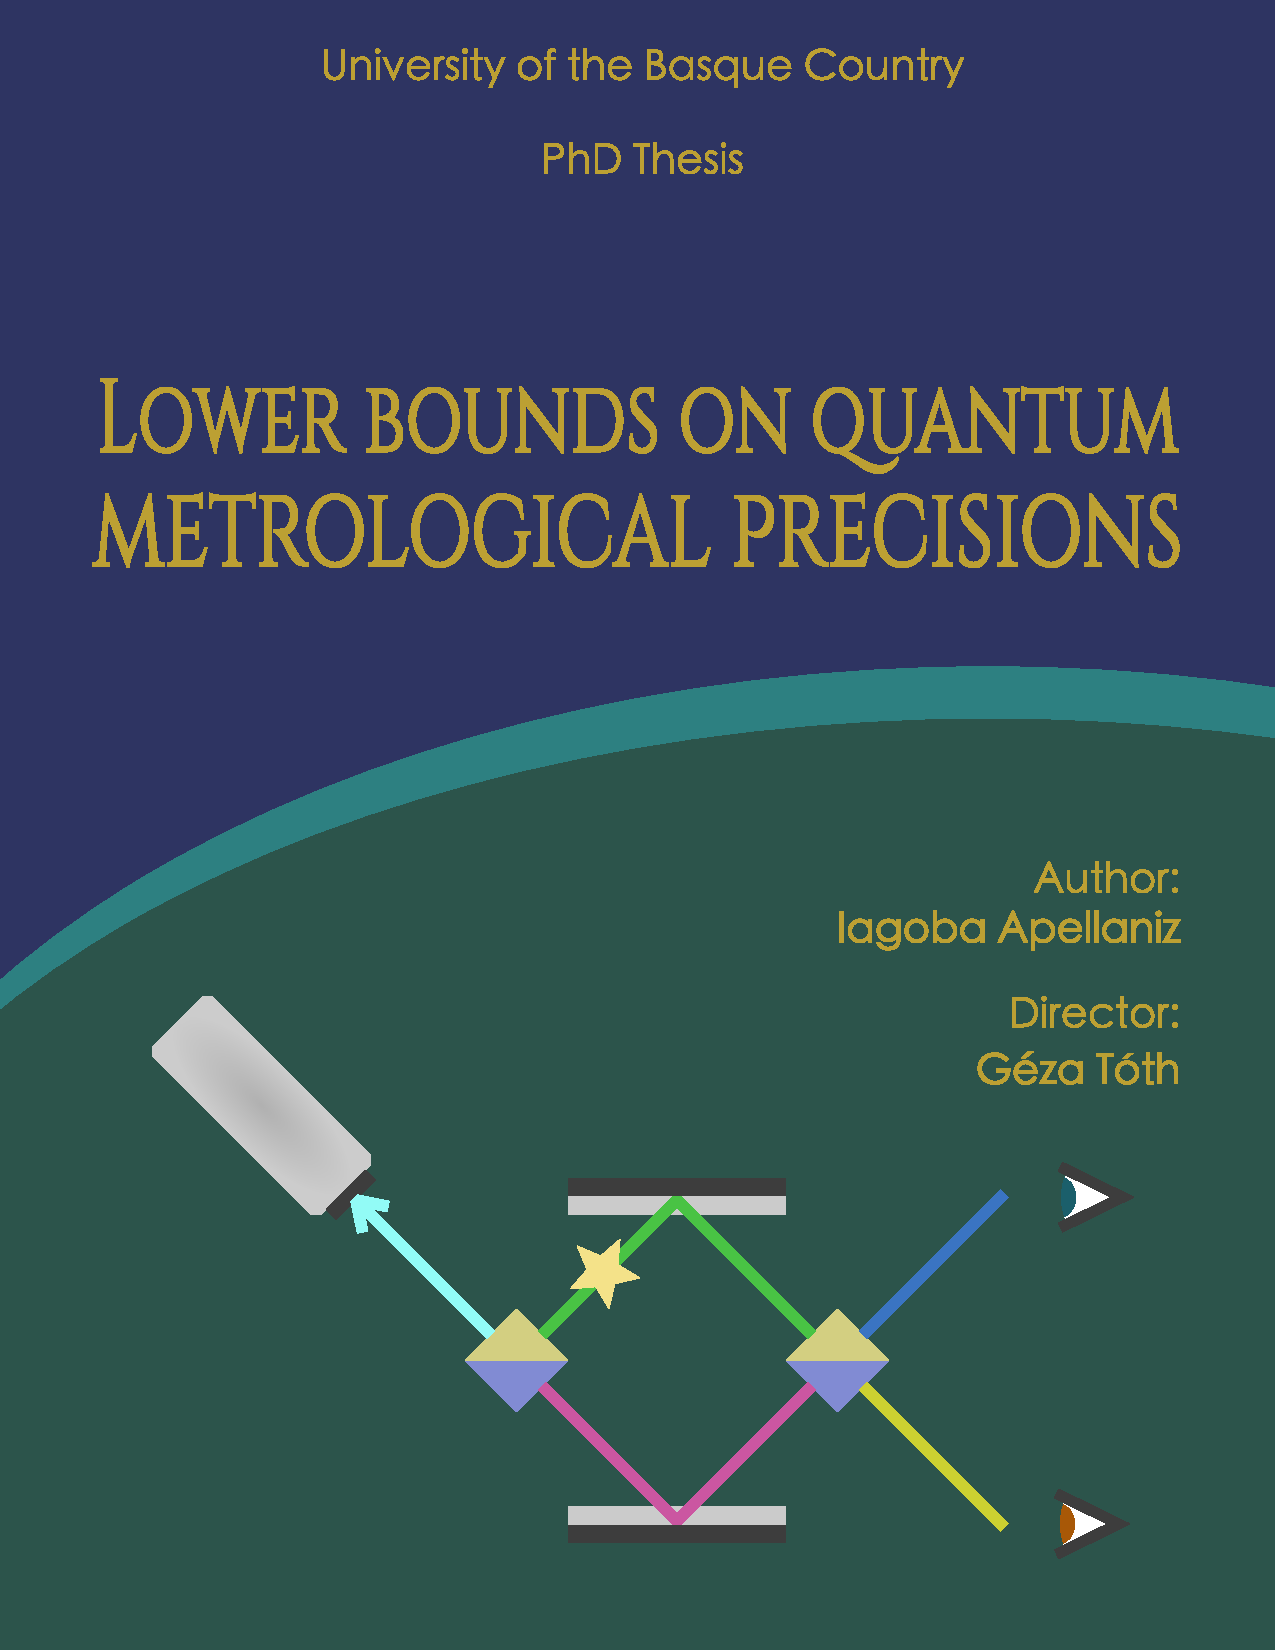
\includepdf[pages=-, offset=72 -36]{img/cover.pdf}

%%%%%%%%%%%%%%%%%%%%%%%%
% EDITION TIPS
%%%%%%%%%%%%%%%%%%%%%%%%

\cleardoublepage

This document was generated with the 2014 distribution of \LaTeX.

\vfill


\includegraphics[height=20pt]{img/0-CreativeCommons-by-sa.png}

2012-2015 Iagoba Apellaniz. This work is licensed under the Creative Commons
Attribution-ShareAlike 4.0 International License. To view a copy of this
license, visit
\href{http://creativecommons.org/licenses/by-sa/4.0/deed.en_US}
{http://creativecommons.org/ licenses/by-sa/4.0/deed.en\_US}.
\clearpage

%%%%%%%%%%%%%%%%%%%%%%%%
% PROLOGE
%%%%%%%%%%%%%%%%%%%%%%%%

\section*{Prologue}
\setcounter{page}{1}
\pagenumbering{roman}
\fancyfoot[LE,RO]{\thepage}

\lettrine[lines=2, findent=3pt,nindent=0pt]{T}{his} work is part of the doctoral project on Quantum Information which I started on the sumer of 2013.
This work collects part of the research I have done on these previous years.
I will try to be clear throughout all the thesis such that make it readable for a wider audience as it is possible.
This way I hope it will be readable by any person with a bachelor in science, particularly in physics or at least with a partial knowledge in Quantum Mechanics.
With that in mind the first and the second chapters will be used to introduce the reader into the context on which this thesis was written as well as the basic notions of Quantum Metrology, the enveloping field of the present work.
Even though I write this thesis for a broad audience in mind, a basic notion on quantum physics and statistics is needed to follow it properly as I said before.
For instance, I will assume among other things that the reader knows what probability is and which are its properties, or what a quantum state is and what it represents.
I will give references where to find such complementary material when I think is necessary.

This research I publish in a thesis form is part of the work done within the Research Group in Quantum Information in which Prof.
G\'eza T\'oth is the group leader and principal investigator.
I have to mentions the rest of the members of the group Dr. Philipp Hyllus, Dr. Giuseppe Vitagliano, Dr. I\~nigo Urizar-Lanz, Dr. Zolt\'an Zinbor\'as and Dr. Matthias Kleinmann at the time I was working on the projects of this thesis.
Some of them may still be part of the group and some not.
Apart from the group of G\'eza T\'oth based in Bilbao, Spain, this thesis also collects some work done in collaboration with the Theoretical Quantum Optics (TQO) group lead by Prof. Otfried G\"uhne at the University of Siegen, Germany, and the group of Prof. Carsten Klempt at the Leibniz University in Hannover, based also in Germany.
The last one is an experimental group specialized on the creation of exotic quantum states with very many particles with a variety of applications in quantum technology.

First, we investigate the metrological usefulness of a family of states known as the unpolarized Dicke states, which have boosted the sensitivity of magnetometry when lots of particles are used in the sense that quantum enhancements play a very important role to achieve such a precision.
Second, we investigate possible lower bounds on the quantum Fisher information, a quantity that characterizes the usefulness of a state for quantum metrology, using the theory of Legendre transforms such that we obtain thight lower bounds based on few measurements of the initial quantum state that will be used for metrology.
And last but not least, we investigate the gradient magnetometry, i.e., we develop a theory to study the capablilities of some states to sense the change in space of the magnetic field and we apply that theory to some known states.

Before the thesis work the reader can find the present prologue, the list of publications, the table of contents, and a list of abbreviations, figures and tables.
Then, the thesis starts.
On the first pages one can find a brief dedicatory and acknowledgements followed by the chapters.
The content of the chapters is organized as follows.
First, I start with an introduction to describe the current situation of Quantum Information spetially Quantum Metrology and I write about the basics of Quantum Metrology and how it emerges from statics and Quantum Mechanics.
Second, I present the reader our works in characterizing the family of states known as the unpolarized Dicke states, in optimizing the lower bound for the quantum Fisher information when some expectation values of the states are known and our work in gradient quantum metrology.

\begin{flushright}
  Iagoba Apellaniz

  Bilbao, \today
\end{flushright}


\section*{Publications}
{\setlength{\parindent}{0cm}
Iagoba Apellaniz \textit{et al}, \textit{New J. Phys.} \textbf{17} 083027 (2015)

Detecting metrologically useful entanglement in the vicinity of Dicke states
\vspace{10pt}

G\'eza T\'oth and Iagoba Apellaniz, \textit{J. Phys. A: Math. Theor.} \textbf{47} 424006 (2014)

Quantum metrology from a quantum information science prespective

\subsection*{Preprints}
\subsection*{Out of the scope of this thesis}

Giuseppe Vitagliano \textit{et al} 2014 \textit{Phys. Rev. A} \textbf{89} 032307

Spin squeezing and entanglement for an arbitrary spin
}
%%%%%%%%%%%%%%%%%%%%%%%%
% TABLE OF CONTENTS
%%%%%%%%%%%%%%%%%%%%%%%%

\vspace*{100pt}
\tableofcontents

%%%%%%%%%%%%%%%%%%%%%%%%
% FIGURES TABLES, ETC
%%%%%%%%%%%%%%%%%%%%%%%%
\section*{Tables, figures and abbreviations}
\fancyfoot[LE,RO]{\thepage}

[Insert in a table]

SLD - Symmetric logarithmic derivative.

QFI - Quantum Fisher information

%%%%%%%%%%%%%%%%%%%%%%%%
% THESIS
%%%%%%%%%%%%%%%%%%%%%%%%

\cleardoublepage

\pagenumbering{arabic}
\fancyfoot{}
%!TEX root = main.tex 

\thiswatermark{\centering
\put(0,-110){
\includegraphics[height=2.5cm]{img/0-Ztf.png}} 
\put(430,-100){
\includegraphics[height=2cm]{img/0-Ehu.png}}
} 

\begin{center}

\vspace*{20pt}
\textsc{\LARGE University of the Basque Country}

\vspace{20pt}
\textsc{\Large PhD Thesis}

\vspace{50pt} 
\hrule 

\vspace{16pt}
{\huge \bfseries Lower bounds on quantum metrological precisions}
\vspace{16pt}

\hrule
\vspace{40pt}

\begin{minipage}{0.4\textwidth}
\begin{flushleft} \large
\emph{Author:}


M. Sc. Iagoba \textsc{Apellaniz}
\end{flushleft}
\end{minipage}
\begin{minipage}{0.4\textwidth}
\begin{flushright} \large
\emph{Director:}

Prof. G\'eza \textsc{T\'oth} %TODO: Check Geza's name
\end{flushright}
\end{minipage}

\vspace{40pt}
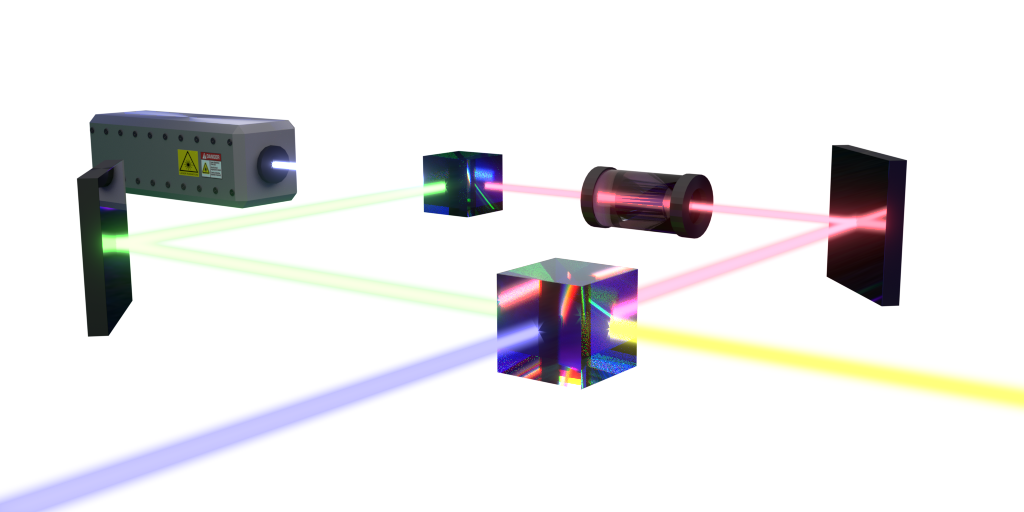
\includegraphics[width=0.8\hsize]{img/cover3Dpicture.png}
\vfill

% Bottom of the page
{\large \today}

\end{center}

\cleardoublepage
\cleardoublepage
\setcounter{page}{1}

%%%%%%%%%%%%%%%%%%%%%%%%
% DEDICATION PAGE
%%%%%%%%%%%%%%%%%%%%%%%%
\vspace*{100pt}
\begin{center}
\emph{To my parents, my family}

\emph{and to all the people}

\emph{I have had around me those years.}
\end{center}

\cleardoublepage

\section*{Acknowledgments}

I want to thank the people that support me in this endeavor especially my office and discussion mates and my director G\'eza T\'oth for without whom my work would not be even  started.
I also want to thank more people especially those from the theoretical physics department of the University of the Basque Country and the unique very especial group for me from the Theoretical Quantum Optics group at the University of Siegen.
I would really like to mention the names of all of them but I think it would be quite heavy for the average reader of this thesis.
Thank you guys!
Also I want to thank people from the group QSTAR at Florence, Italy.

On the other hand I also felt very comfortable at my university, the University of the Basque Country, but I want to thank especially the people that make me grow in all ways as person.

\cleardoublepage

%%%%%%%%%%%%%%%%%%%%%%%%
% HEADINGS AND PAGE NUM.
%%%%%%%%%%%%%%%%%%%%%%%%

\renewcommand{\rightmark}{\bf \thesubsection}
\renewcommand{\headrulewidth}{0.5pt}
\fancyfoot[LE,RO]{\thepage}
\fancyhead[LE]{Section: \rightmark} % TODO: Solve heading
\fancyhead[RO]{\leftmark}

%%%%%%%%%%%%%%%%%%%%%%%%
% REDEFINE TITLE FORMAT
%%%%%%%%%%%%%%%%%%%%%%%%
\titleformat{\section}[display]
{\vspace*{150pt}
\bf\Huge}
{\hspace{-72pt}{\textcolor{grey}{\thesection}} \hspace{36pt} {\textcolor{white}{#1}}}
{0pt}
{}
[]
\titlespacing*{\section}{108pt}{10pt}{60pt}[16pt]


%%%%%%%%%%%%%%%%%%%%%%%%
\section{Introduction}
\thiswatermark{\put(1,-241){\color{l-grey}\rule{84pt}{48pt}}
\put(84,-241){\color{grey}\rule{410pt}{48pt}}}


%!TEX root = main.tex

% Section: Introduction
\lettrine[lines=2, findent=3pt,nindent=0pt]{M}{etrology} has played an inportant role since [TODO: add historical reasons]. With the development of quantum technology, a more deep understanding of one of its aspect as the quantum metrology is needed. Therefore, many works appeared recently on the literature. 

In this work the author, in collaboration with other researchers [TODO: see how to add reference to the rest of collavorators], has addressed some crucial questions regarding this field. 

%%%%%%%%%%%%%%%%%%%%%%%%
\section[Backgroud on Quantum Metrology]
{Development of Quantum Metrology}
\thiswatermark{\put(1,-241){\color{l-grey}\rule{84pt}{48pt}}
\put(84,-241){\color{grey}\rule{410pt}{48pt}}}


\section[Backgroud on Quantum Metrology]
{Background on Quantum Metrology}
\thiswatermark{\put(1,-241){\color{l-grey}\rule{84pt}{48pt}}
\put(84,-241){\color{grey}\rule{410pt}{48pt}}}


\quotes{Roger J. Barlow}{In the real world, doing real experiments, statistics began to matter}

\vspace{0pt}
\lettrine[lines=2, findent=3pt,nindent=0pt]{I}{n} this chapter we will study the basics of Quantum Metrology, which stands for the science of enhanced metrology by quantum phenomena.
On the other hand, metrology, as the science of measuring, has played an essential role for the development of the technology as we know it today.
It studies several aspects of the estimation process, such as which strategy to follow in order to improve the precision of an estimation or which is the bound for the precision.
Metrology also covers all intermediate process fo the estimation, from the design aspects of a precise measuring device, to the most basic concepts of estimation, which lead at the end to a better understanding of it as a whole.

In this sense, with the discovery of the Quantum Physics and the development of Quantum Mechanics, new doors for advances in metrology were open in the early decades of the 20th century.
First, Quantum Theory embrased the so-called field of Quantum Information, which merges the notions of the theory of information and computer science, among others subfields, with the quantum mechanics.
This new field of Quantum Information is in the basis of Quantum Metrology.
Moreover, those emerging fields rapidly became into very interesting interdisciplinary playgrounds of science attracting the interest of many scientists as well as resources for their researches.
Just to menetion that the role of the so-called entanglement, an exclusive feature of Quantum Mechanics which cannot be completelly described using classical probabilistic theories, is essential in this context.
With the aim of completelly understand this concepts, many scientists world wide have integrated their efforts.
Said this, the entanglement also is in the center of theoretical concepts in Quantum Metrology.
In the Quantum Metrology framework, we will focus on the achievable precision of the systems.
We will show as well different strategies to achieve the desired results.

On the other hand, a very important field of science must be highlighted by its own meriths.
We are mentioning the statistics, without which many descriptions of the actual and past physical findings would lack of the rigorous interpretation needed for the complexity of data samples.
It basically helps to analyse raw data to find special properties out of it.

\subsection{Background on statistics and the theory of estimation}

In this section, we will enumerate the basic concepts of statistics as well as the estimation process.
As we said, the main mathematical tools used by the metrology science belong to statistics.
Moreover, we are expecially interested in estimation theory.
The statistics main characteristic is that it makes the raw data under consideration comprehensible from the human perspective.
The data can be anything, from a set of different heights of a basketball team, to the outcomes of a coin toss, or the wavelength of photons coming out of some sample.
The aim of this section is to give the reader sufficient material to follow this thesis and make it comprehensible from the beginning\footnote{
For a more detailed material, check statistics book as weel as mathematics book for scientist and engeneers \citep{Riley1998, BarlowXXXX}}.

\subsubsection{Probability, data samples, average and variance}

The probability indicates the relative chance of an event to happen.
For instance, if there is a box with ten red balls and five blue balls, considering that the balls of the same color are indistinguishable and that we extract one randomly, we have $\frac{5}{10+5}=\frac{1}{3}$ of probability to obtain a blue ball and $\frac{2}{3}$ to obtain a red ball.
The reader may notice many properties a probability should have, such as that the probability of any event to happen is always one or that a probability is always given by a number in between zero and one.
For more details, there are many interesting textbooks or chapters of some textbook about Probability Theory one could follow if interested.
The following References~\citep{Riley1998, BarlowXXXX} are some of those books.

When someone has a data sample at hand, it might come from diverse sources and might be represented using multiple forms such as numbers or words (for instace, a table of names of people), the first thing one tries to accomplish is to analyse the data to extract the relevant properties from it.
A data sample always come from a population sample, i.e., the data sample might not be complete (one could lose some in the process) neither exact (a measuring device always have an error when estimating a magnitude).
Hence, the data sample comes attached with a probability for each data element.
In the subsecuent paragraphs, we will describe this relation and we will enumenrate the most useful properties and formulas for the comprehensions of this thesis.

First of all, we will explain our notation which follows the one used on Reference~\citep{Riley1998}.
A probability function gives the probability of an event $x$ to happen when measuring some random variable $X$, and it is denoted by $\prob(X=x)$.
Second, the $N$ elements of a data sample are considered to come from $N$ random variables with the corresponding $N$ values due to the random nature of the measuring, $\{X_i=x_i\}_{i=1}^N$.
The joint probability of those random variables is in general not separable.
This is due to the fact that the outcomes could depend on the rest of the outcomes or some other more complex relation that makes the most general case to be non-separable from the probabilistic point of view.
Therefore we define this PDF as an $N$ variable function
\be
  \prob(\bs{X}=\bs{x}) \equiv \prob(X_1=x_1,X_2=x_2,\dots,X_N=x_N).
\ee
If separable this is written by
\be
  \prob(\bs{X}=\bs{x}) = \prod_{i=1}^N\prob(X_i=x_i)
\ee
and it is the case for many relevan cases.

When some property of the system is defined as a function of random variables, the result is also a random variable with another transformed PDF.
For example, we measure the position of a body at some moment.
If the system was at rest on the origin at initial time and the acceleration is known to be constant, then from the position one can infeer on the value of the acceleration by using $A=2X/t^2$, where $X$ denotes the position at intant $t$ and $A$ the acceleration.
If $X$ is a random variable, which is the general case when measuring the position of a body, then the probability is computed in this case by
\be
  \prob(A=a) = \frac{\text{d}x}{\text{d}a}\prob(X=x)=\frac{2}{t^2}\prob(X=x).
\ee
In general for the multiple random variable case transformations, we must require that
\be
  |\prob(\bs{X}=\bs{x})\,\text{d}x_1\text{d}x_2\dots\text{d}x_N|=|\prob(\bs{Y}=\bs{y})\,\text{d}y_1\text{d}y_2\dots\text{d}y_N|.
\ee
This leads to some interesting formulas we will discuss later.

We now stick to the simplest case on which the data is a collection of values of the same random variable describing the same physical one-dimensional data population.
Some definitions reasonable to mention in this thesis arise for those kind of data samples: the average, variance, moments and central moments.
The arithmetic average (there are other types of average one can find in the textbooks) is computed by
\be
  \overline{x}=\frac{1}{N}\sum x_i.
\ee
The variance is related with the spread of the data and computed by
\be
  \sigma^2=\frac{1}{N}\sum (x_i-\overline{x})^2,
\ee
where $\sigma$ is the standard deviation.
Different moments are computed by $\overline{x^r}=\frac{1}{N}\sum x_i^r$ while central moments are of the form of $n_r=\frac{1}{N}\sum (x_i-\overline{x})^r$.
Notice that the variance is the second central moment of the data sample.
For completeness, when each element of the data consists of more than a number, e.g., $(x_i,y_i,z_i)$, the covariance between two data kinds, in the following case $X$ and $Y$, is obtained by
\be
  V_{X,Y} = \frac{1}{N}\sum_{i=1}^N (x_i-\overline{x})(y_i-\overline{y}).
\ee

Those functions also apply to the probability distribution functions.
While these last ones may be unkown functions for us, as soon as we collect all the possible data or we are in the large number regime the variances of the data sample and of the data population, the means, the covariances and so on so forth, they must coincide.
We will try to keep this distinghusion as clear as possible.
In general the mean values of any function over data sample values $g(x)$ are denoted with a bar over a lowercase variable, e.g., $\overline{x^r}$ for the $r$-th moment, while the mean values of any function applied to the data population $g(X)$ is written following some textbooks by $\text{E}[g(X)]$.
One clearlly may distinguish two cases here: one for continuous functions where the expectation values or the means are computed integrating over all the posible values, and the other case on which $\prob(\bs{X}=\bs{x})$ can take only discrete values.
For completeness here are the two definitions
\be
  \text{E}[g(\bs{X})] = \lcor
  \begin{split}
    &\int g(\bs{x}) \prob(\bs{X}=\bs{x})\,\text{d}^N \bs{x},\\
    &\sum_{i,j,\dots} g(\bs{x}) \prob(\bs{X}=\bs{x}).
  \end{split}
  \right.
\ee
One more deffinition needs our attention and it is the variance any function $g(X)$ denoted by $\text{V}[g(X)] \equiv \text{E}[g(X)^2] - E[g(X)]^2$.

\subsubsection{Frecuentist vs. bayesian approach}

\subsubsection{Estimators and Fisher information}

Let us supose that the data sample has encoded some wanted parameters $\bs{a}\equiv(a_1,a_2,\dots)$.
The underlying probability, in general also unknown, may be conditioned by the real values of the wanted parameters $\bs{a}$.
The probability of the data sample is therefore writen as
\be
  \prob(\bs{X}=\bs{x}|\bs{a}),
\ee
where "$|\bs{a}$" indicates its dependency on these parameters.
At this point, notice that an estimate of the the wanted parameter based on the data sample has the form of a function the random variables.
Therefore as mentioned before, an estimator of $a$, which is how is called this quantity and is denoted by $\hat{a}$, is another random variable with a PDF of the form of
\be
  \prob(\hat{a}|\bs{a})\,\text{d}\hat{a} = \prob(\bs{X}=\bs{x}|\bs{a})\,\text{d}x_1\text{d}x_2\dots\text{d}x_N.
\ee
For short, we omit on writing $\bs{X}$ from now on, thus the conditional joint pobrability of $N$ random variables is written as $\prob(\bs{x}|\bs{a})$.

As we said, an estimator is defined to be a function of the data sample.
For example, one of such estimators is the estimator of the mean value of the data population, in general unknown.
The mean value of the data population, which in general we do not have acces to, is denoted usually by $\mu$.
Notice that $\mu$ is in general different from the mean value of the data sample $\overline{x}$.
A valid estimator for the population mean value would be the arithmetic mean of the data sample, i.e., $\hat{\mu}=\overline{x}$.

An important notion of an estimator is its \emph{efficiency}, i.e., whether it has smaller variance than another.
The more efficient estimator the smaller variance it has.
Remember than an estimator is a random variable so it must have a variance that comes from the data population, i.e., from $\prob(\hat{a}|\bs{a})$ in this case.

For an estimator of any kind there is a theoretical lower bound for its variance.
For the proof of the previous observation, which we compute for continuous random variables without lossing of generality, we start with the normalisation of the PDF
\be
  \int \prob(\bs{x}|\bs{a})\,\text{d}^N\bs{x} = 1.
\ee
Next, we compute the partial derivate over $a$ such that
\be
  \int \partial_a\prob(\bs{x}|\bs{a})\,\text{d}^N\bs{x} = \int \partial_a\big(\ln  \prob(\bs{x}|\bs{a})\big) \prob(\bs{x}|\bs{a}) \,\text{d}^N\bs{x} = 0,
\ee
where for simplification, we ommit the arguments of the joint probability on the second equality.
From Eq.~\eqref{}, it turns out that the Eq.~\eqref{} is the expectation value of $\partial_a(\ln\prob)$.
Finally if we have an unbiashed estimator, for which the true value $a$ coincides with the expectation value of the estimator $\text{E}[\hat{a}]$, its partial differenciation over $a$ must be equal to one,
\begin{align}
  \partial_a\text{E}[\hat{a}] &= \partial_a a = 1, \\
  \begin{split}
    1 &= \partial_a \int \hat{a} \prob(\bs{x}|\bs{a})\,\text{d}^N\bs{x} \\
      &=  \int \hat{a} \partial_a\prob(\bs{x}|\bs{a})\,\text{d}^N\bs{x} =  \int \hat{a} \partial_a\big(\ln  \prob(\bs{x}|\bs{a})\big) \prob(\bs{x}|\bs{a}) \,\text{d}^N\bs{x},
  \end{split}
\end{align}
where we apply the definition of the expectation value of the estimator $\hat{a}$ for continuous variables and we apply as well similar identities as in Eq.~\eqref{}.

At this point we invoke the Schwarz inequallity for two real multidimensional functions $g(\bs{x})$ and $h(\bs{x})$ such that $(\int g h \,\text{d}^N\bs{x})^2\leq (\int g^2 \,\text{d}^N\bs{x}) (\int h^2 \,\text{d}^N\bs{x})$.
With this we can follow the following receipe to obtain a lower bound for the variance of a general estimator.
First the deffinition of the variance looks like
\be
  V[\hat{a}] = E[(\hat{a}-a)^2] = \int (\hat{a} - a)^2\prob(\bs{x}|\bs{a})\,\text{d}^N\bs{x}.
\ee
Second, from Eqs.~\eqref{,} holds that
\be
  \int (\hat{a}-a)\partial_a\big(\ln  \prob(\bs{x}|\bs{a})\big) \prob(\bs{x}|\bs{a})\,\text{d}^N\bs{x} = 1
\ee
because $a$ is not a function of $\bs{x}$.
Hence, using the Schwarz inequality we can write
\be
  \text{V}[\hat{a}] = \int (\hat{a} - a)^2\prob(\bs{x}|\bs{a})\,\text{d}^N\bs{x} \geq \frac{1}{\int \lcua\partial_a\big(\ln \prob (\bs{x}|\bs{a}) \big)\rcua^2 \prob (\bs{x}|\bs{a})\,\text{d}^N\bs{x}},
\ee
which is also known as the Cramer-Rao bound or the Fisher inequality.

With this review on the interesting features of "classical" metrology, we conclude this section.
In the next section, we recall some properties of the Quantum Mechanics and we subsecuentelly follow with the basis of Quantum Metrology. 




\subsection{Quantum Mechanics from metrology perspective}

The ubiquitous probabilistic nature of quantum mechanics forces all the community to know some basics on probability and statistics.

\subsubsection{The quantum state, multi-particle state, entanglement}

A \emph{system state} in Quantum Mechanics lives on a Hilbert space, $\mathcal{H}$.
The system state, $\rho$, has the following properties:
\begin{enumerate}
  \item
  It is Hermitian, so it is invariant under the complex transposition, $\rho=\rho^\dagger$.
  \item Its trace is equal to one, $\tr(\rho)=1$.
  \item It is positive semi-definite, i.e, all its eigenvalues are bigger or equal to zero, $\rho=\sum_{\lambda}p_\lambda \Pi_\lambda$\footnote{
    $\rho=\sum_{\lambda}p_\lambda \Pi_{\lambda}$ is the eigen-representation of the state, where $\Pi_{\lambda}$ are the eigenstates defined on $\mathcal{H}$ too.
    They are as many as the dimension, $d$, of the Hilbert space.
    They are orthonormal under the product defined on such Hilbert space $\mathcal{H}$, i.e, $\tr(\Pi_{\lambda}\Pi_{\lambda'})=\delta_{\lambda,\lambda'}$.
    Nevertheless, there is a extended discussion when Hilbert space is defined for continuous variables, see [XXX].
  } where $p_\lambda\geq 0$ are the scalar eigenvalues.
  It follows that $\sum_\lambda p_\lambda = 1$.
  \item If all $p_\lambda$ are zero except one, the state is a pure state, $\rho=\Pi_\lambda$.
  \item It follows that the quantum states form a convex set where the extremal points are pure states.
\end{enumerate}


The composite system of $N$ different parties lives on $\mathcal{H} = \mathcal{H}^{(1)}\otimes\mathcal{H}^{(2)}\otimes\cdots\otimes\mathcal{H}^{(N)}$ or for short $\mathcal{H} = \bigotimes_{i=1}^N\mathcal{H}^{(i)}$, where $\otimes$ stands for a tensor product like construction.
For instance, this composite Hilbert space could be used to represent a many-particle system, in this case $N$ particles.
A \emph{separable} state on this Hilbert space can be described in the following way,
\be
  \rho = \sum_{i}p_i\rho_i^{(1)}\otimes\rho_i^{(2)}\otimes\cdots\otimes\rho_i^{(N)},
\ee
where $p_i$ are convex weights that sum to one and are equal or bigger than zero.
If not the state is said to be \emph{entangled}.


Angular momentum operators.
The angular momentum algebra comes

Entanglement cannot be described classically.

Evolution

Unitary evolution

Markov

Limblad

Measurements (POVM)

Quantum Information

\subsection{Quantum Metrology}

The evolution of a quantum state can be used to infer on some hidden parameter.
The estimation theory applied to the intrinsic statistical nature of a quantum states has lead to the the formulation of Quantum Metrology as an important subfield.
Merging the probabilistic features of quantum mechanics and the estimation theory is not trivial.
Nevertheless, starting from the pioneering works of Wotters, Braunstein and some other I probably forgot to mention [XXX] were the statistical distance of neighbor states is studied we have lead to amazing results which today drive many experiments and technology.
From the works of Giovannetti et al and Paris on the middle of the last decade fundamental concepts arose, for example the figure of merit quantum Fisher information or the Heisenberg limit.
In this section we will highlight the most important aspects of this field and with this we will conclude this introductory chapter.

The error propagation formula for an estimation of $\Theta$ based on the observable $O$.
\be
  (\Delta \Theta)^2 \geq \frac{\varian{O}}{|\partial_{\Theta}\expect{O}|^2}
\ee

\subsubsection{Quantum Magnetometry}
\label{sec:bg-quantum-metro}

One of the most basic tasks of Quantum Metrology is to address the precision of estimating the magnetic field strength, namely $B$, of an unknown external magnetic field.
In this section we will assume that the magnetic field is homogeneous on the position space.
To consider more advanced situations on which the magnetic field changes linearly with the position, see chapter [XXX].
With the aim of estimating the strength of the magnetic field, a prove state is used in order to interact with it, coupling the magnetic moment of the state and the field itself.
After some time, the state has evolved.
Finally, measuring how the state has changed one would be able to infer on the strength of the magnetic field, basically proportional to the change on the state.

In general, we will say that the magnetic moments of the states come exclusively from the spin angular momentum, neglecting any possible contribution from the orbital angular momentum.
This way the physics is simpler.
This is justified in the sense that most of the recent experiments on this context have been carried out with ion-traps, BECs or at most cold atomic ensembles, which have indeed a negligible orbital angular momentum.

Beside this considerations, the interaction Hamiltonian can be written as,
\be
  H = - \bs{\mu} \cdot \bs{B}
\ee
up to some constant factor.
Now in the simplest case we will choose the magnetic field to be pointing to some fixed direction, for instance, the $z$-direction.
So the magnetic field vector can be written as ${B}=B\bs{k}$, where $\bs{k}$ is the unitary vector pointing to the $z$-direction.
This way estimation problem is much more simple, since one has not to determine the direction of the magnetic field.

The magnetic moment of the system is proportional to the spin angular momentum, $\bs{\mu}=-\mu_\text{B} g_{\text{s}}\hbar^{-1} \bs{J}$, where $\mu_{\text{B}}$ and $g_{\text{s}}$ are the Bohr magneton and anomalous gyromagnetic factor respectively.
Finally, one can rewrite the interaction Hamiltonian as,
\be
  H = \gamma B J_z
\ee
where $\gamma = \mu_\text{B} g_{\text{s}}\hbar^{-1}$ and we have used the fact that $\bs{J}\cdot\bs{k}=J_z$.
Finally, the unitary operator leading the evolution of the system can be written as,
\be
  U = \exp(-i\Theta J_z),
\ee
where the magnetic field strength is encoded into the variable $\Theta=-\mu_\text{B} g_\text{s} t B/\hbar$.
Here $\mu_\text{B}$ stand for the Magneton of Bhor and $g_\text{s}$ for the giro-magnetic constant for the spin angular momentum, and $t$ is the time spent on the evolution.

\begin{figure}
  \centering
  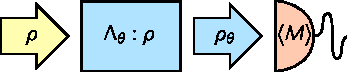
\includegraphics[scale=.85]{img/BG_preparation_encoding_estimation.pdf}
  \caption[Quantum Metrology estimation process]{Secuence of the different steps for the basics of the estimation process on Quantum Metrology. First, an input state $\rho$ enters the region on which the unknown parameter $\Theta$ is imprinted on it, for the most general case, representented with $\Lambda_{\Theta}$. Last, the state that has encoded the parameter $\Theta$ on it is measured and $\Theta$ must be infered from the measured quantity $\expect{M}$.}
  \label{fig:bg-preparation-encoding-estimation}
\end{figure}

\begin{figure}
  \centering
  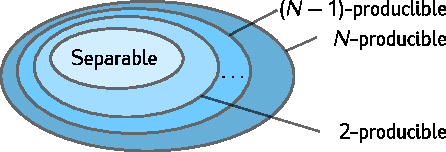
\includegraphics[scale=.85]{img/BG_separability_k_producibility_circle.pdf}
  \caption[Diagram for $k$-producibility sets]{}
  \label{fig:bg-separability-k-producibility-circle}
\end{figure}

\be
  \label{eq:bg-pezze-bound}
  \qfi[\rho,J_z] \geq \frac{\expect{J_y}^2}{\varian{J_x}}
\ee


%%%%%%%%%%%%%%%%%%%%%%%%
\section[Quantum metrology with Dike like states]
{Metrology in the vicinity of Dicke states}
\thiswatermark{\put(1,-282){\color{l-grey}\rule{84pt}{88pt}}
\put(84,-282){\color{grey}\rule{410pt}{88pt}}}


\lettrine[lines=2, findent=3pt,nindent=0pt]{I}{n} this chapter we will present recent results regarding the metrological usefulness of a family of unpolarised states.
Such states can be used as prove states to estimate the homogeneous magnetic field strength, see Section~\ref{sec:bg-quantum-metro}.

One of the figures of merit of this such unpolarized, but still useful states is the so-called unpolarized Dicke state [XXX], which consists of, on its $Oz$-axis  representation, an equal number of qubits pointing up and pointing down while the whole state is at the same time symmetrised.
It can be written as follows,
\be
  \ket{\text{D}_N^{0}} \equiv \ket{\text{D}_{N}}:= \binom{N}{N/2}^{-\frac{1}{2}}
  \sum_{k\in \sigma_\text{s}}
  P_{k}\left( \ket{1}^{\otimes N/2} \ket{0}^{\otimes N/2}
  \right),
  \label{eq:vd-unpolarised-dicke}
\ee
where $k$ are elements of the set of all possible unique symmetric permutations $\sigma_\text{s}$.
This state is also called twin-fock state on different contexts.
Such state is known to be highly entangled [XXX] and to reach Heisenberg scaling when used in magnetometry.
For these and other reasons unpolarised Dicke states have been created in photonic systems [XXX], in cold-gases [XXX] and recently in trapped ions [XXX].

The symmetric subspace of $N$ spin-$\frac{1}{2}$ particles is decomposed in $N+1$ orthonormal states, see Appendix~\ref{app:angular-subspaces} for more details on how such subspaces behave even for different spins.
Indeed, the subspace can be seen as a single spin-$\frac{N}{2}$ particle.

One of the most particular features this state has is that since it is a eigenstate of the collective operator $J_z$ with corresponding eigenvalue equal to zero.
At the same time, it lives on the subspace where the collective total spin is maximum\ie $\expect{\bs{J}^2}=N(N+2)/4$.
Thus, with this together with the fact that the state is unpolarised, it turns that it must have a very large uncertainty for the collective spin operators perpendicular to $J_z$, namely $J_x$ and $J_y$.

\subsection{Unpolarised states for magnetometry}

Having unpolarised states for magnetometry has been shown useful in Section~XX.
While the quantum Fisher information would give directly the performance one state would have, this is not feasible in general because a complete knowledge of the state is needed to compute such value.
On the other hand, we can use the error propagation formula Equation~(XX) to obtain a bound on the precision.
As one can see on the Figure~\ref{fig:vd-secuence-evo} a pure Dicke state is rotated along the $Oz$-axis.
Say that in this case the initial state is an unpolarised Dicke state of aligned with the $Ox$-axis.
\begin{figure}
  \centering
  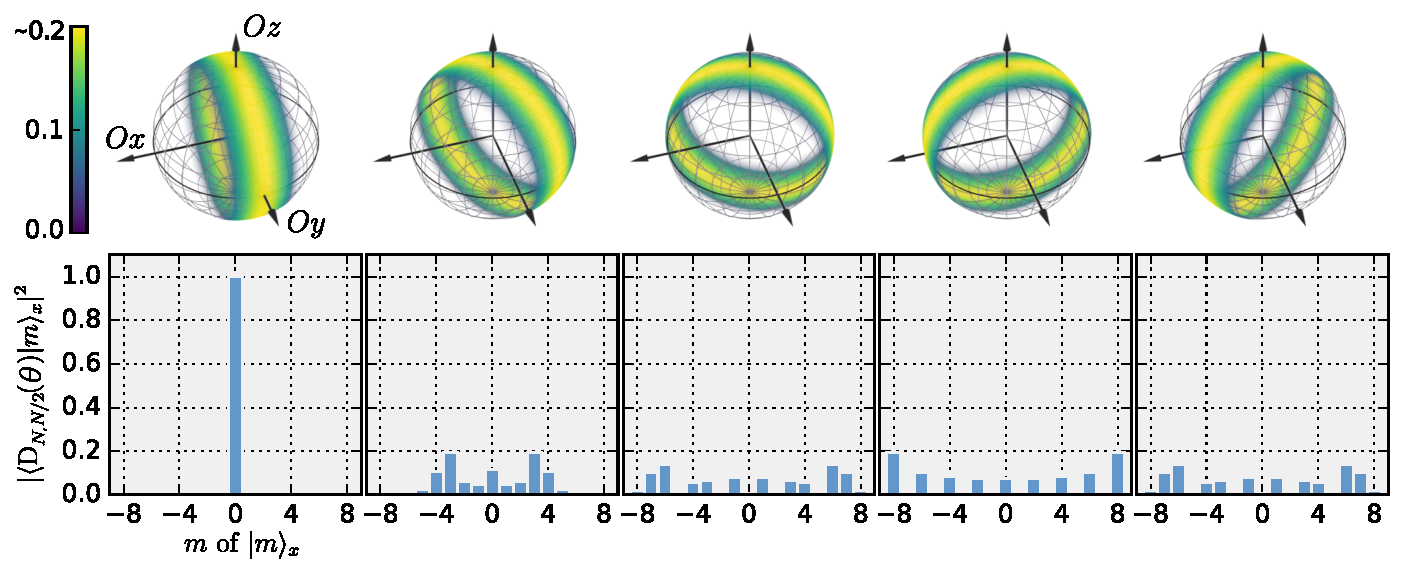
\includegraphics[scale=.65]{img/plots/VD_evolution_of_dicke.pdf}
  \caption{Secuence of the evolution of an unpolarized Dicke state of 16 qubits for $\Theta=\{i\pi/6\}_{i=0}^4$. Bloch spheres representing the Hirusi distribution of the state, and below PDF of the $J_x$ POVM for each step of the secuence}
  \label{fig:vd-secuence-evo}
\end{figure}

The state initially is an eigenstate of the $J_x^k$ operators for $\forall k \in [1,\infty]$.
Another feature of the sequence is that $\expect{J_l}=0$ for $\forall l\in x,y,z$.
It turns out that measuring the evolution of the second statistical moment of $J_x$ is one of the ways to go.
It will start having value equal to zero for the pure unpolarized Dicke state, and rapidly will increase its value as it can be seen on the Figure~\ref{fig:vd-secuence-evo}.
Another heuristic observation is that for $\Theta=\pi/2$ the value of $\expect{J_x^2}$ will be at its maximum been it proportional to $\expect{\bs{J}^2}$ so to $N^2$.
Hence, the change on the second moment over the phase shift must be in this case proportional to $N^2$.
From this and for those states, we lead to the conclusion that one only needs to measure the second moment of the collective spin $J_x$ to observe precisions that scale with the Heisenberg limit.
In the following equation we show the error propagation formula that will give us the obtained precision,
\be
  \varian{\Theta} = \frac{\varian{J_x^2}}{|\partial_{\Theta} \expect{J_x}|^2}.
  \label{eq:vd-error-propagation}
\ee

\subsection{Evolution of the expectation values}
With the aim of computing the precision, Equation~{(\ref{eq:vd-error-propagation})}, we will compute the dependence on $\Theta$ of the expectation value of the operator $J_x$ and higher order moments.
For that first of all we will move onto the Heisenberg picture where the operators evolve in time while the state remains the same.
The operator $J_x$ can be written a a function of $\Theta$ the following way,
\be
  J_x(\Theta) = e^{i \Theta J_z} J_x(0) e^{-i \Theta J_z} = J_x(0) \text{c}_\Theta - J_y(0) \text{s}_{\Theta},
\ee
where $J_l(0)$ for $\forall l$ are the collective angular momentum operators at time equal zero, which we will write them simply $J_l$ from now on, and $\text{c}_\Theta$ and $\text{s}_\Theta$ are the trigonometric functions introduced on the first chapter.

We need to compute the second and the fourth moments of $J_x$ as it is required by the Equation~{(\ref{eq:vd-error-propagation})}.
But before any calculation we will make a simplifying assumption which turn to be well supported on the most common situations.
The assumption is that both expectation values are even functions on $\Theta$,
\be
  \begin{split}
    \expect{J_x^2(\Theta)} &=\expect{J_x^2(-\Theta)}, \\
    \expect{J_x^4(\Theta)} &=\expect{J_x^4(-\Theta)}.
  \end{split}
  \label{eq:vd-even-f-constraint}
\ee

The square of $J_x$ in the Heisenberg picture is written as follows,
\be
  J_x^2(\Theta)= J_x^2 \text{c}_\Theta^2 + J_y^2 \text{s}_\Theta^2
  - (J_xJ_y + J_yJ_x) \text{c}_\Theta\text{s}_\Theta.
\ee
From the equation above and to fulfill the first constraint on the Equation~{(\ref{eq:vd-even-f-constraint})} it turns out that the expectation value over our yet to be shown initial state of the operator $(J_xJ_y + J_yJ_x)$ must vanish.
Hence it is equivalent to the first assumption of the Equation~{(\ref{eq:vd-even-f-constraint})} write that
\be
  \expect{\{J_x,J_y\}} = 0
  \label{eq:vd-init-2nd-constraint}
\ee
where $\{\, ,\,\}$ stands for the anticommutator.
Apart for been simpler to compute the Equation~{(\ref{eq:vd-init-2nd-constraint})} is based also on initial expectation values of the state.
We will see that as we said before this is easily guarantied for most important cases.

As we have done recently with the square of $J_x$ now we will do it for $J_x^4$.
This way one will be able to distinguish which other combination of operators must vanish in order to have Equation~{(\ref{eq:vd-even-f-constraint})} guarantied. The fourth power of $J_x$ can be written as follows in the Heisenberg picture,
\begin{multline}
  J_x^4(\Theta)= J_x^4 \text{c}_\Theta^4 + J_y^4 \text{s}_\Theta^4
  + (J_x^2J_y^2 + J_xJ_yJ_xJ_y + J_xJ_y^2J_x + J_yJ_xJ_yJ_x + J_yJ_x^2J_y + J_y^2J_x^2) \text{c}_\Theta^2\text{s}_\Theta^2 \\
  -(J_x^3J_y+J_x^2J_yJ_x+J_xJ_yJ_x^2+J_yJ_x^3)\text{c}_\Theta^3\text{s}_\Theta
  -(J_xJ_y^3+J_yJ_xJ_y^2+J_y^2J_xJ_y+J_y^3J_x)\text{c}_\Theta\text{s}_\Theta^3.
\end{multline}
And again assuming that its expectation value must be an even function on $\Theta$ it turns out that the second line must be equal to zero when the expectation value is considered.
So $(J_x^3J_y+J_x^2J_yJ_x+J_xJ_yJ_x^2+J_yJ_x^3)$ and $(J_xJ_y^3+J_yJ_xJ_y^2+J_y^2J_xJ_y+J_y^3J_x)$ must vanish again over any candidate state to be used as prove state.
Hence, the second constraint of the Equation~{(\ref{eq:vd-even-f-constraint})} can be rewritten as follows,
\be
  \begin{split}
    \expect{\big\{J_x^2 , \{ J_x,J_y\}\big\}}=0,\\
    \expect{\big\{J_y^2 , \{ J_x,J_y\}\big\}}=0.
  \end{split}
\ee

Finally, we can write how the evolution of second and fourth moments of the $J_x$ operator must look like,
\begin{align}
  \expect{J_x^2(\Theta)}=\; &\expect{J_x^2} \text{c}_\Theta^2 + \expect{J_y^2} \text{s}_\Theta^2
  \label{eq:vd-evo-2nd-moment}\\
  \begin{split}
    \expect{J_x^4(\Theta)}=\; &
    \expect{J_x^4}\text{c}_\Theta^4 + \expect{J_y^4} \text{s}_\Theta^4 \\
    & + \expect{\{J_x^2,J_y^2\}+\{J_x,J_y\}^2} \text{c}_\Theta^2\text{s}_\Theta^2.
  \end{split}
\end{align}
From here we are able to write the evolution of the variance of the second moment when Equation~{(\ref{eq:vd-even-f-constraint})} must be obeyed.
We obtain
\be
  \begin{split}
    \varian{J_x^2(\Theta)} &= \expect{J_x^4(\Theta)} -\expect{J_x^2(\Theta)}^2 \\
    &= \expect{J_x^4}\text{c}_\Theta^4 + \expect{J_y^4} \text{s}_\Theta^4
    + \expect{\{J_x^2,J_y^2\}+\{J_x,J_y\}^2} \text{c}_\Theta^2\text{s}_\Theta^2
    - \big(\expect{J_x^2} \text{c}_\Theta^2 + \expect{J_y^2} \text{s}_\Theta^2\big)^2\\
    &= \big(\expect{J_x^4}-\expect{J_x^2}^2\big)\text{c}_\Theta^4
    + \big(\expect{J_y^4}-  \expect{J_y^2}^2\big)\text{s}_\Theta^4
    + \big(\expect{\{J_x^2,J_y^2\}+\{J_x,J_y\}^2} - 2 \expect{J_x^2}\expect{J_y^2}\big)
    \text{c}_\Theta^2\text{s}_\Theta^2\\
    &=\varian{J_x^2}\text{c}_\Theta^4 + \varian{J_y^2} \text{s}_\Theta^4+ \big(\expect{\{J_x^2,J_y^2\}+\{J_x,J_y\}^2} - 2 \expect{J_x^2}\expect{J_y^2}\big)\text{c}_\Theta^2\text{s}_\Theta^2.
  \end{split}
\ee

The remaining constituent of the Equation~{(\ref{eq:vd-error-propagation})} on which we will base our result for the precision, is the modulus square of the derivative of the second moment of the $J_x$ operator.
Using Equation~{(\ref{eq:vd-evo-2nd-moment}) for the expression of the evolution of the second moment, the denominator of Equation~{(\ref{eq:vd-error-propagation})} follows
\be
  \begin{split}
    |\partial_\Theta \expect{J_x^2(\Theta)}|^2 & = |-2\expect{J_x^2}\text{c}_\Theta\text{s}_\Theta+2\expect{J_y^2}\text{c}_\Theta\text{s}_\Theta|^2\\
    & = 4\expect{J_y^2-J_x^2}^2\text{c}_\Theta^2\text{s}_\Theta^2.
  \end{split}
\ee

From the equations above directly follows expression for the precision of $\Theta$,
\be
\begin{split}
  \varian{\Theta} & = \frac{\varian{J_x^2}\text{c}_\Theta^4 + \varian{J_y^2} \text{s}_\Theta^4+ \big(\expect{\{J_x^2,J_y^2\}+\{J_x,J_y\}^2} - 2 \expect{J_x^2}\expect{J_y^2}\big)\text{c}_\Theta^2\text{s}_\Theta^2}
  {4\expect{J_y^2-J_x^2}^2\text{c}_\Theta^2\text{s}_\Theta^2}\\
  & = \frac{\varian{J_x^2}\text{t}_\Theta^{-2} + \varian{J_y^2} \text{t}_\Theta^2+ \expect{\{J_x^2,J_y^2\}+\{J_x,J_y\}^2} - 2 \expect{J_x^2}\expect{J_y^2}}
  {4\expect{J_y^2-J_x^2}^2}.
\end{split}
\label{eq:vd-result-before-simp}
\ee
To this calculations further computations follows mainly regarding to the following expectation value $\expect{\{J_x^2,J_y^2\}+\{J_x,J_y\}^2}$.
This calculus is left for the Appendix~{\ref{ap:loca-simplification}}.
Finally, the expression Equation~{(\ref{eq:vd-result-before-simp})} leads to the following,
\be
  \varian{\Theta} = \frac{\varian{J_x^2}\text{t}_\Theta^{-2} + \varian{J_y^2} \text{t}_\Theta^2 + 3\expect{J_y^2} - 2 \expect{J_z^2} - 2\expect{J_x^2}(1+\expect{J_y^2}) + 6\expect{J_xJ_y^2J_x}}
  {4\expect{J_y^2-J_x^2}^2}
  \label{eq:vd-precision-as-theta}
\ee
[IT IS SLIGHTLY DIFFERENT FROM THE PUBLICATION..., This difference would make invariant all the results except the plot SPSQ -> QFI vs BOUND, which in this case the bound gets improved!!]

One can realize that the whole dependence on the phase shift is in the first two terms of the numerator.
This way one can minimize the sum on the first two terms in order to find where the precision is best.
So it follows that,
\be
  \tan^2(\Theta_{\text{opt}}) = \sqrt{\frac{\varian{J_x^2}}{\varian{J_y^2}}}
\ee
which inserted on the Equation~{(\ref{eq:vd-precision-as-theta})} gives us the optimal precision when the second moment $\expect{J_x^2}$ is measured based on the initial expectation values of the input state. The optimal precision is written in the following way,
\be
  \varian{\Theta}_{\text{opt}} = \frac{\sqrt{\varian{J_x^2} \varian{J_y^2} } + 3\expect{J_y^2} - 2 \expect{J_z^2} - 2\expect{J_x^2}(1+\expect{J_y^2}) + 6\expect{J_xJ_y^2J_x}}
  {4\expect{J_y^2-J_x^2}^2}.
  \label{eq:vd-precision}
\ee.

We conclude with this section checking our bound for the pure unpolarised Dicke state aligned with $Ox$, $\ket{\text{D}_N}_x$, whose precision bound is well known, Equation~{([XXX])}.
With this aim we compute all the expectation values needed for the Equation~{(\ref{eq:vd-precision})} which almost all of them are trivial, $\expect{J_xJ_y^2J_x}=\expect{J_x^4}=\expect{J_x^2}=0$.
The rest are obtained in the following way,
\begin{align}
  \expect{J_y^2} & = \expect{J_z^2} = \frac{N (N+2)}{8},
  \label{eq:vd-2moment-pure-dicke}\\
  \expect{J_y^4} & = \frac{N+2}{8}\left(\frac{3N(N+2)}{16}-\frac{1}{2}\right).
  \label{eq:vd-4y-moment-pure-dicke}
\end{align}
The Equation~{(\ref{eq:vd-2moment-pure-dicke})} follows directly from the fact that the state is invariant under rotations on the $Ox$ axis, so they are its expectation values, because the sum of all the second moments must give the value of the total angular momentum, in this case the maximum which is $\expect{\bs{J}^2} = \frac{N (N+2)}{4}$, and because $\expect{J_x^2}=0$.
The proof of the Equation~{(\ref{eq:vd-4y-moment-pure-dicke})} needs more algebra and has been left for the Appendix~{\ref{ap:}}.

From the equations above, one lead to the following expression for the precision of the phase shift for a pure unpolarised Dicke state,
\be
  \varian{\Theta} = \frac{2}{N(N+2)},
\ee
which coincides exactly with the inverse quantum Fisher information for such state.

\subsection{Testing the formula against some known states}

In this section we will compare our criteria based on few expectation values against the corresponding quantum Fisher information obtained for some known input states.
Those input states will be first the family of states defined as the ground states of the following Hamiltonian, called the spin-squeezing Hamiltonian,
\be
  H_\lambda = J_x^2 - \lambda J_y.
\ee
For $\lambda$ equal to zero we have the unpolarized Dicke state, Equation~{(\ref{eq:vd-unpolarised-dicke})}, and for $\lambda$ large we recover the coherent totally polarized state pointing onto the $Oy$ direction.
In the meantime the state is also a spin-squeezed state, therefore the name of the Hamiltonian.
The ground state is defined such that
\be
  \lambda_{\min} = \tr(H_\lambda \rho_\lambda),
\ee
where $\lambda_{\min}$ is the lowest eigenvalue of $H_\lambda$.
The state $\rho_\lambda$ is invariant under permutations of the particles and it is also pure.
Moreover the state $\rho_\lambda$ is symmetric.

The second family of input states we are going use are the Gaussian mixture of Dicke states around the unpolarized Dicke state, which have the following form as function of $\beta$,
\be
  \rho_{(T)} \propto \sum_{m=-N/2}^{N/2} e^{- \frac{m^2}{T}} \ket{\text{D}_N^m}_x\bra{\text{D}_N^m}_x.
\ee

\begin{figure}
  \centering
  \igwithlabel{(a)}{scale=.65}{img/plots/VD_against_spsq.pdf}
  \igwithlabel{(b)}{scale=.65}{img/plots/VD_against_therm.pdf}
  \caption{Comparison between our formula for the precision and the QFI for different states. (a) Comparison for ground states of $H_\lambda$. (b) Comparison with gaussian mixture of Dicke states.}
  \label{fig:bg-histograms}
\end{figure}

After showing how the optimal precision formula behaves compared with the quantum Fisher information for those two families of states, we also have to proof that they indeed fulfill the constraints on Equation~{(\ref{eq:vd-even-f-constraint})}.

For the spin-squeezed state , $\rho_\lambda$, we have that it is invariant under

On the other hand for the thermal state, $\rho_T$, we have that it is invariant under rotations around the $Ox$ axis
\be
  \rho_T = e^{-i \alpha J_x} \rho_T e^{i \alpha J_x},
\ee
for arbitrary $\forall \alpha$.

\be
  \tr(e^{i\Theta J_z}J_y^m e^{-i\Theta J_z}\rho_T) = \tr(e^{i\Theta J_z}J_y^m e^{-i\Theta J_z} e^{-i \alpha J_x} \rho_T e^{i \alpha J_x})
\ee

If we choose $\alpha = \pi$ then we rotate all the orthogonal angular momentum operators such that $J_y \rightarrow - J_x$ and $J_z \rightarrow -J_z$.
Therefore, $e^{i \pi J_x}e^{i\Theta J_z}J_y^m e^{-i\Theta J_z} e^{-i \pi J_x}=e^{-i\Theta J_z}(-J_y)^m e^{i\Theta J_z}$.
Hence, for even $m$ and particularly for $m=2,4$ we have that,
\be
  \tr(e^{i\Theta J_z}J_y^m e^{-i\Theta J_z}\rho_T) = \tr(e^{-i\Theta J_z}J_y^m e^{i\Theta J_z}\rho_T ),
\ee
so the Equation~{(XXX)} is granted.

\subsection{Using our method with real experimental data}

On reference [XXX], it is produced on the laboratory a state with the proper characteristics of an unpolarised Dicke state, small variance on one of the directions and very large one on the perpendicular directions to this.
It is also invariant under rotations around $Ox$-axis.
Effectively, the state has the following form,
\be
  \rho = \frac{1}{2\pi}\int e^{-i\alpha J_x} \rho_0 e^{i\alpha J_x},
\ee
where $\rho_0$is what we would obtain if we would have access to the phase reference.
Hence we have that at $\Theta=0$ all the statistical moments $\expect{J_z^m}=\expect{J_y^m}$ are equal.

Simplification of our precision formula on Equation~{(XXX)}.
First, we simplify the expectation value $\expect{J_xJ_z^2J_x}$ in the following way,
\be
\begin{split}
  \expect{J_xJ_y^2J_x} &= \frac{\expect{J_x (J_y^2 + J_z^2)J_x}}{2}
  =\frac{\expect{J_x (J_x^2 + J_y^2 + J_z^2 )J_x} - \expect{J_x^4}}{2} \\
  & \leq \frac{N(N+2)}{8} \expect{J_x^2} - \frac{\expect{J_x^4}}{2}.
\end{split}
\ee
Notice that obtaining $\expect{J_xJ_z^2J_x}$ is hard experimentally.
This simplification can only make our estimation of the precision worse while for symmetric states the equality holds.
The bound from below for the precision can be writtes as,
\be
  \varian{\Theta}_{\text{opt}} \leq \frac{\sqrt{\varian{J_x^2} \varian{J_y^2} } + \expect{J_y^2} + \frac{3N(N+2)-8}{4} \expect{J_x^2} - 2\expect{J_x^2}\expect{J_y^2} - 3\expect{J_x^4}}
  {4\expect{J_y^2-J_x^2}^2},
\ee
where some terms were reordered and further simplified.

It is worth to study this case and apply our methods such that we can extract conclusions about the metrological usefulness of the state.
The system in consideration is a $N=7900$ particles system.
The measured data for such system is
\be
\begin{aligned}
  \expect{J_x^2} & = 112 \pm 31, \\
  \expect{J_x^4} & = 40 \times 10^3 \pm 22 \times 10^3,
\end{aligned}
\quad
\begin{aligned}
  \expect{J_y^2} & = 6 \times 10^6 \pm 0.6 \times 10^6, \\
  \expect{J_y^4} & = 6.2 \times 10^{13} \pm 0.8 \times 10^{13}.
\end{aligned}
\ee
Hence we obtain the maximum precision,
\be
  \frac{(\Delta \Theta)^{-2}_{\text{opt}}}{N} \geq 3.7 \pm 1.5
\ee
with boot straping methods.
The direct substitution would yield to a 3.3 gain over the shot-noise limit.

Next we plot the value for the precision substituting directly the measured data into Equation~{(XXX)}, see Figure~\ref{fig:vd-precision-theta}.
\begin{figure}
  \centering
  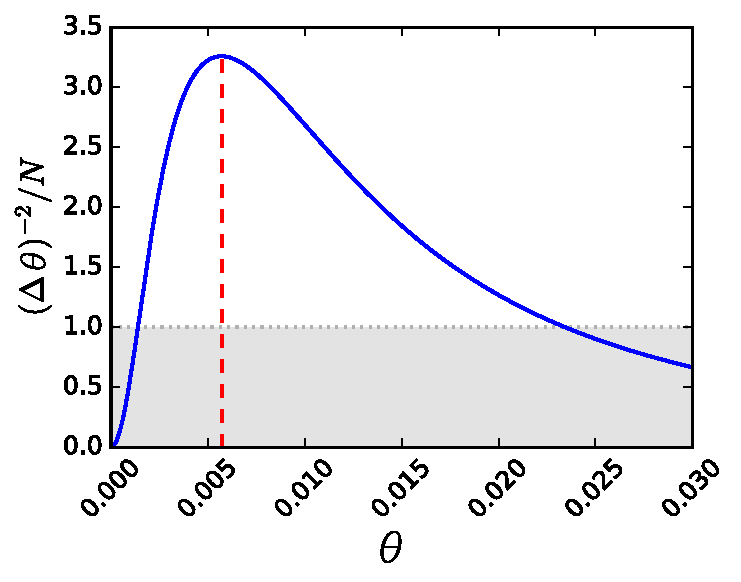
\includegraphics[scale=.65]{img/plots/VD_precision_theta.pdf}
  \caption{The (solid) line shows how the precision of $\Theta$ varies through the evolution. Notice that for the initial moment the precision is zero and that it reaches a maximum at $\Theta \approx 0.0057$ highlighted with the vertical (dashed) line. The gray area represent the region where the precision is below the shot-noise limit.}
  \label{fig:vd-precision-theta}
\end{figure}

Further simplification of our method can be achieved for states of the kind of the one studied on this section.
Based on $\expect{AB}\leq\lambda_{\max}(A)\expect{B}$ for two commuting positive-semidefinite observables,
\be
  \expect{J_y^4}\leq\frac{N^2}{4}\expect{J_x^2}.
\ee

We can also approximate $\expect{J_x^4}$ with $\expect{J_x^2}$ in the sense that it is small and that mainly its value comes from technical noise,
\be
  \expect{J_x^4} \approx \beta \expect{J_x^2}^2.
\ee
This approximation even if it is not a strict bound on the precision can be very useful in order to characterize the metrological usefulness of our input state based only on second statistical moments of only two angular momentum operators, namely $\expect{J_z^2}$ and $\expect{J_x^2}$.
Those two expectation values are related with the width of our state and also with how thin we can do it in one of the directions, for metrological purposes, perpendicular to the magnetic field.
So in this case we use $\beta=3$ assuming that the distribution function has Gaussian shape.

From these considerations we are able to write a second bound with fewer expectation values for the optimal precision such that,
\be
  \varian{\Theta}_{\text{opt}} \leq \frac{\expect{J_y^2} + \frac{3N(N+2)-8}{4} \expect{J_x^2} + \Big(\sqrt{\frac{N^2}{2\expect{J_y^2}}-2} - 2 \Big) \expect{J_y^2}\expect{J_x^2} - 9\expect{J_x^2}^2}
  {4\expect{J_y^2-J_x^2}^2}.
\ee
We have used this formula to compute the bound on the optimal precision with the measured data shown on Equation~{(XXX)}, $(\Delta \Theta)^{-2}_{\text{opt}} \geq 2.9N$, see Figure~{\ref{fig:vd-experimental}}.

\begin{figure}
  \centering
  \igwithlabel{(a)}{scale=.65}{img/plots/VD_exper_contour.pdf}
  \igwithlabel{(b)}{scale=.65}{img/plots/VD_exper_slice.pdf}
  \caption{Comparison between our formula for the precision and the QFI for different states. a) Comparison for ground states of $H_\lambda$. (b) Comparison with gaussian mixture of Dicke states.}
  \label{fig:vd-experimental}
\end{figure}


%%%%%%%%%%%%%%%%%%%%%%%%
\section[Bounds on QFI with observables]
{Bounding the QFI with few initial expectation values}
\thiswatermark{\put(1,-282){\color{l-grey}\rule{84pt}{88pt}}
\put(84,-282){\color{grey}\rule{410pt}{88pt}}}



\section[Witnessing metrologically useful entanglement]
{Witnessing metrologically useful {\color{grey} X} entanglement}
\label{sec:lt}
\thiswatermark{\put(1,-282){\color{l-grey}\rule{84pt}{88pt}}
\put(84,-282){\color{grey}\rule{410pt}{88pt}}}


\quotes{Adrien-Marie Legendre}{All the truths of mathematics are linked to each other,

and all means of discovering them are equally admissible.}

\lettrine[lines=2, findent=3pt,nindent=0pt]{T}{ypically}, one has no access to the density matrix of the system which is used for metrology or for some other quantum information processing task.
Moreover, for systems in which the particle number is very large, which is the case when one wants to do metrology with quantum states, the details of the density matrix cannot be known due to practical reasons.
Since the quantum Fisher information is based on the complete knowledge of the density matrix, methods to avoid the complete tomography must be developed as we have shown a practical case in the previous chapter.
In this chapter, we obtain a general procedure to get an optimal bound for the quantum Fisher information based on as many expectation values of the initial state as one is ready to measure.
Two main features are worth to mention again.
First, in general this method gives us an optimal tight bound.
Second, the bound is based on the expectation values of the initial state only, so it is not necessary to perform an evolution of the state.
This is in contrast to other approaches one can find in the literature, ours needs a significantly smaller experimental effort.

From Eq.~\eqref{eq:bg-pezze-bound}, a lower bound on the quantum Fisher information based on expectation values of the initial state is
\be
  \qfif{\rho,J_z} \geqslant \frac{\expect{J_x}^2}{\varian{J_y}}.
\ee
where the state is polarized along the $x$-axis \cite{Pezze2009}.
In the previous chapter we have also shown one of these bounds specifically designed for unpolarized Dicke states \eqref{eq:vd-unpolarized-dicke}.

The setup is described in Section~\ref{sec:bg-quantum-magnetometry} and consists of in estimating the homogeneous magnetic field strength, in this case, which points towards the $z$-axis.
Therefore, we will base our calculations on the quantum Fisher information $\qfif{\rho, J_z}$, defined in Eqs.~\eqref{eq:bg-qfi-definition-eigen-decomposition} and \eqref{eq:bg-qfi-definition-convex-roof}, see Section~\ref{sec:bg-qfi} for more information about the properties of the QFI.

\subsection{Lower bound on a convex function given some arbitrary expectation values}

Our problem could be solved with Lagrange multipliers or Legendre transforms.
We follow the method based on Legendre transforms, since the problem of getting a lower bound of a convex function on the states having already some expectation values of some arbitrary observables has already been studied by O. G\"uhne {\it et al.} and J. Eisert {\it et al.} in Refs.~\cite{Guehne2007, Eisert2007} respectively, mainly from the perspective of entanglement measures.
The illustrated techniques are based on the well known Legendre transform for differentiable functions, see Appendix~\ref{app:legendre-transform} for more details.
We first review in this section the state-of-the-art solution to this problem.
And later on, we extend it to the quantum Fisher information.
For simplicity in the next section, Section~\ref{sec:lt-transform-for-single-observable}, we assume that a single expectation value is given.
An extension to the case in which more expectation values are given will follow in the Section~\ref{sec:lt-transform-for-m-observables}.
Finally, we will summarize our results with an explicit formula which will be used to compute the bounds in the most general case.

\subsubsection{Estimation of a general convex function based on the expectation value of an arbitrary observable}
\label{sec:lt-transform-for-single-observable}

When a convex function $g(\rho)$ is given together with an expectation value of some operator $w=\tr(\rho W)$, a tight lower bound, $\bound{g}(w)$, can be obtained as \cite{Rockafellar1996, Guehne2007, Eisert2007}
\be
  \label{eq:lt-lower-bound-single-parameter}
  \begin{split}
    g(\rho)\geqslant\bound{g}(w):=\,&\sup_r \{ rw - \hat{g}(rW)\}\\
    =\,& \{\inf_{\rho}g(\rho)\,|\,w = \tr(\rho W)\},
  \end{split}
\ee
where $\hat{g}(rW)$ is the Legendre transform of $g(\rho)$ and the second equality expresses the tightness of the bound.
The Legendre transform in this context is defined as
\be
  \label{eq:lt-for-convex-function-single-parameter}
  \hat{g}(rW)=\sup_{\rho}\{\expect{rW}_\rho - g(\rho)\},
\ee
where the maximization is over \emph{all} possible states.
This method to obtain the lower bound has been used to compute entanglement measures \cite{Guehne2007, Eisert2007}.

Following the theory one can find that in the case in which the convex function $g(\rho)$ is defined as a convex roof over all possible convex decompositions of the state, the optimisation of Eq.~\eqref{eq:lt-for-convex-function-single-parameter} can be reduced to an optimization over pure states only, thus simplifying the calculation \cite{Guehne2007, Eisert2007}
\be
\begin{split}
  \hat{g}(rW) & = \sup_{\rho}\{\expect{rW}_\rho - g(\rho)\} \\
  &=\sup_{\rho}\Big\{r\expect{W}_\rho - \inf_{\{p_k,\ket{\phi_k}\}}\big\{\sum_{k} p_k g(\ket{\phi_k})\big\} \Big\} \\
  &=\sup_{\{p_k, \ket{\phi_k}\}} \Big\{ \sum_k p_k \expect{rW}_{\ket{\phi_k}} - \inf_{\{p_k, \ket{\phi_k}\}} \big\{\sum_k p_k g(\ket{\phi_k}) \big\}  \Big\} \\
  &=\sup_{\{p_k, \ket{\phi_k}\}} \Big\{ \sum_k p_k \big\{ \expect{rW}_{\ket{\phi_k}} - g(\ket{\phi_k}) \big\} \Big\} \\
  &=\sup_{\ket{\psi}} \big\{ \expect{rW}_{\ket{\psi}} - g(\ket{\psi}) \big\}.
\end{split}
\ee
However, even an optimization over all pure states is feasible numerically only for small systems.
We will show later in this section how to circumvent this problem in the case of the QFI.
The convex roof construction has the following form
\be
  g(\rho) = \inf_{\{p_k,\psi_k\}} \sum_{k}p_k g(\ket{\psi_k}),
\ee
where the mixed state is decomposed into $\rho = \sum_k p_k \ketbra{\psi_k}{\psi_k}$.
Among other definitions of the QFI in the literature, there is one that defines it as the convex roof of $4\varian{J_z}$, the variance of the generator, as it has been shown on Ref.~\cite{Toth2007, Yu2013}, we can compute the Legendre transform optimizing for pure states only.
Hence, we will be able to use this simplification to apply this method to obtain the lower bound on the QFI.
Note that in this context, the QFI is the convex roof of four times the variance of the generator, Eq.~\eqref{eq:bg-qfi-definition-convex-roof}.

\subsubsection{Measuring several observables}
\label{sec:lt-transform-for-m-observables}

For some cases, it is interesting to characterize the quantum state not only with a single measurement but with several.
For instance, we might want to use, as it is done with the spin-squeezed states the absolute polarization and the variance of one of the orthogonal components of the angular momentum to detect entanglement and metrological usefulness \cite{Pezze2009}.
So far, we studied the case in which a single measurement is used.
Its extension to several expectation values is indeed straight-forward.
We can generalize Eqs.~\eqref{eq:lt-lower-bound-single-parameter} and \eqref{eq:lt-for-convex-function-single-parameter} for several observables $\{W_i\}_{i=1}^M$ as follows \cite{Guehne2007}
\be
  \label{eq:lt-extension-bound-multiparameter}
  \bound{g}(w_1,w_2,\dots) := \sup_{\bs{r}}\big\{\bs{rw}-\sup_{\rho}\{\expect{\bs{rW}}-g(\rho)\}\big\},
\ee
where $\bs{ab} =\sum_{k=1}^M a_kb_k$, the usual notation for scalar products of two vectors.

\subsubsection{Explicit form of the expression to be optimized}

After we have shown how to find a lower bound for a general convex function of the state based on its expectation values and how to simplify that method for the case in which the function is defined as a convex roof, now we are in the position to achieve the main goal of this chapter.
First of all, we note that for the quantum Fisher Information the inner maximization, the Legendre transform, is obtained optimizing a function quadratic in expectation values,
\be
\label{eq:lt-legendre-of-qfi}
\begin{split}
  \hat{\qfi}(rW) &= \sup_{\ket{\psi}}\big\{r\expect{W}_{\psi}-4\varian{J_z}_{\psi}\big\} \\
  &= \sup_{\ket{\psi}} \big\{ r\expect{W}_{\psi}-4\expect{J_z^2}_{\psi} + 4\expect{J_z}^2_{\psi} \big\} \\
  &= \sup_{\ket{\psi}} \big\{\expect{rW-4J_z^2}_{\psi} +
  \expect{2J_z}^2_{\psi}\big\},
\end{split}
\ee
where we have used the fact that the QFI can be expressed as a convex roof of $\varian{J_z}$ and we arrive at the problem of an optimization over a single parameter for simplicity on the following derivations.
Equation~\eqref{eq:lt-legendre-of-qfi} can be rewritten as an optimization linear in operator expectation values and over a parameter $\mu$ as
\be
  \hat{\mathcal{F}}_{\text{Q}}(rW) = \sup_{\ket{\psi},\mu}\big\{\expect{rW-4J_z^2}_{\psi}+8\mu\expect{J_z}_\psi - 4 \mu^2\mtxid\big\},
\ee
which, making use of $\max\{\expect{A}\}=\lambda_{\max}[A]$ for any observable, can be reformulated as
\be
  \label{eq:lt-legendre-for-qfi-simplified}
  \begin{split}
    \hat{\mathcal{F}}_{\text{Q}}(rW) & = \sup_{\ket{\psi}}\big\{\lambda_{\max}[rW-4J_z^2+8\mu J_z - 4 \mu^2]\big\}\\
    &=\sup_{\ket{\psi}}\big\{\lambda_{\max}[rW-4(J_z-\mu)^2]\big\},
  \end{split}
\ee
where we omitted in writing $\mtxid$ for clarity and $\lambda_{\max}[A]$ stands for the maximum eigenvalue of the operator $A$.
At the extremum, the derivative with respect to $\mu$ must be zero, hence at the optimum $\mu=\expect{J_z}_{\text{opt}}$ which represents the expectation value of $J_z$ should have considering the optimal state in Eq.~\eqref{eq:lt-legendre-of-qfi}.
This also means that we have to test $\mu$ values in the interval $-N/2\leqslant\mu\leqslant N/2$ only for spin-half systems.

The full optimization problem to be solved consists of Eqs.~\eqref{eq:lt-lower-bound-single-parameter} and~\eqref{eq:lt-legendre-for-qfi-simplified} substituting $g(\rho)$ by $\qfif{\rho,J_z}$,
\be
  \bound{\mathcal{F}}(w) = \sup_r\big\{rw-\sup_{\mu}\{\lambda_{\max}[rW-4(J_z-\mu)^2]\}\big\}.
  \label{eq:lt-bound-for-qfi}
\ee
It is crucial that the optimization over $r$ is a concave function, since the theory tells us that $\hat{\mathcal{F}}_{\text{Q}}(rW)$ is a convex function \cite{Rockafellar1996}, even when the multi-parameter case is considered.
Thus the optimum can be determined easily with simple methods, e.g., the gradient method, looking for the maximum in $r$.
Based on Eq.~\eqref{eq:lt-lower-bound-single-parameter}, we can see that even if we do not find the global optimum in $r$, we obtain a valid lower bound.
The extension of this bound to the multi-parameter case is done using the recipe given in Eq.~\eqref{eq:lt-extension-bound-multiparameter}.
On the other hand, the function to be optimized for $\mu$ does not have a single maximum in general.
Moreover, not finding the optimal $\mu$ leads to an overestimating of the bound.
Thus, a large care must be taken when optimizing over $\mu$.

We stress again the generality of these findings beyond linear interferometers covered on the following sections.
For nonlinear interferometers \cite{Luis2004, Boixo2007, Choi2008, Roy2008, Napolitano2011, Hall2012}, the phase $\theta$ must be estimated assuming unitary dynamics $U=\exp{-iG\theta}$, where $G$ is not a sum of single spin operators, hence, it is different from the angular momentum components.

Next, we will demonstrate the use of our approach for several experimentally relevant situations.
In the many-particle case, often symmetric operators can be used to describe accurately the system, which makes it possible to carry out calculations for thousand of particles, as will be presented later in this chapter.

\subsection{Examples}
\label{sec:lt-examples}

In this section, we show how to obtain lower bounds based on the fidelities with respect to the GHZ state and the unpolarized Dicke state as well as with different set of powers of collective angular momentum operators, e.g., the set $\{\expect{J_y}, \expect{J_x}, \expect{J_x^2}\}$.

\subsubsection{Exploiting symmetries}
\label{sec:lt-symmetries}

When making calculations for quantum systems with an increasing number of qubits, we soon run into difficulties when computing the largest eigenvalue of Eq.~\eqref{eq:lt-legendre-for-qfi-simplified}.
The reason is that for $N$ qubits, we need to handle $2^N \times 2^N$ size matrices, hence we are limited to systems of 10 to 15 qubits.

We can obtain bounds for much larger particle numbers, if we restrict ourselves to the symmetric subspace \cite{Toth2007, Toth2009a}.
This approach can give optimal bounds for many systems, such as Bose-Einstein condensates of two-level atoms, which are in a symmetric multiparticle state.
The bound computed for the symmetric subspace might not be correct and generally might overestimate the real bound for general cases.

Finally, it is important to note that if the operators $W_k$ are permutationally invariant (PI) and the eigenstate with the maximal eigenvalue in Eq.~\eqref{eq:lt-legendre-for-qfi-simplified} is non-degenerate, then, we can do the computations on the symmetric subspace only.
The resulting maximal eigenvalue is the maximal eigenvalue when the whole Hilbert space is taken into account for the maximization.
Hence, the lower bound obtained in the symmetric subspace is valid even for the general case.

We follow presenting the proof of the recently mentioned observation for completeness.
Let us denote the ground state of a permutationally invariant Hamiltonian by $\ket{\Psi}$
This is at the same time the $T=0$ thermal ground state, hence it must be a permutationally invariant pure state.
For such states $S_{kl}\ketbra{\Psi}{\Psi}S_{kl}=\ketbra{\Psi}{\Psi}$, where $S_{kl}$ is the swap operator exchanging qubits $k$ and $l$.
Based on this, follows that $S_{kl}\ket{\Psi}=c_{kl}\ket{\Psi}$, and $c_{kl}\in {-1,+1}$.
There are three possible cases to consider:
\begin{enumerate}
  \item All $c_{kl}=+1$.
  In this case, for all permutation operator $\Pi_j$ we have
  \be
    \label{eq:lt-permutating-ground-state}
    \Pi_j \ket{\Psi} = \ket{\Psi},
  \ee
  since any permutation operator $\Pi_j$ can be constructed as $\Pi_j=\prod_i S_{k_il_i}$.
  Equation~\eqref{eq:lt-permutating-ground-state} means that the state $\ket{\Psi}$ is symmetric.
  \item All $c_{kl}=-1$.
  This means that the state is anti-symmetric, however this state exists only for $N=2$ qubits.
  \item Not all $c_{kl}$ are identical to each other.
  In this case, there must be $k_+,l_+,k_-,k_-$ such that
  \be
    \label{eq:lt-different-index-pi}
    \begin{split}
      S_{k_+,l_+} \ket{\Psi} & = +\ket{\Psi},\\
      S_{k_-,l_-} \ket{\Psi} & = -\ket{\Psi}.
    \end{split}
  \ee
  Let us assume that $k_+,l_+,k_-,l_-$ are index different from each other.
  In this case, $\ket{\Psi'}=S_{k_+,k_-}S_{l_+,l_-}\ket{\Psi}$ another ground state of the Hamiltonian $H$ such that
  \be
    \label{eq:lt-different-index-pi-2}
    \begin{split}
      S_{k_+,l_+} \ket{\Psi'} & = -\ket{\Psi'},\\
      S_{k_-,l_-} \ket{\Psi'} & = +\ket{\Psi'}.
    \end{split}
  \ee
  Comparing Eqs.~\eqref{eq:lt-different-index-pi} and \eqref{eq:lt-different-index-pi-2} we can conclude that $\ket{\Psi'}\neq\ket{\Psi}$, while due to the permutational invariance of $H$ we have that $\expect{H}_{\Psi'} = \expect{H}_{\Psi}$.
  Thus, $\ket{\Psi}$ is not a non-degenerate ground state.
  The proof works in an analogous way for the only nontrivial case $k_+=k_-$, when $S_{k_+,k_-}=\mtxid$.
\end{enumerate}

Hence, if $N>2$ then only i) is possible and $\ket{\Psi}$ must be symmetric.

\subsubsection{Fidelity measurements}
\label{sec:lt-bounds-fidelity}

Let us consider the case when $W$ is a projector onto a pure quantum state.
First, we consider GHZ states.
Hence $W$ is the projector $\ketbra{\ghz}{\ghz}$, where
\be
  \ket{\ghz} = \tfrac{1}{\sqrt{2}}(\ket{0\cdots0}+\ket{1\cdots1})
  \label{eq:lt-ghz-state}
\ee
for spin-$\frac{1}{2}$ particles, and $\expect{W}=F_{\ghz}$ is the fidelity with respect to the GHZ state.
Based on knowing $F_{\ghz}$, we would like to estimate $\qfif{\rho,J_z}$\footnote{
Not a tight lower bounds on the quantum Fisher information based on the fidelity have been presented in \cite{Augusiak2016}.}.

Using Eq.~\eqref{eq:lt-bound-for-qfi}, we will obtain an analytical tight lower bound on the QFI based on the fidelity $F_{\ghz}$. The calculation that we have to carry out is computing the bound
\be
  \label{eq:lt-maximization-problem-fid-ghz}
  \bound{\mathcal{F}}(F_{\ghz}) = \sup_r \big\{r F_{\ghz} - \sup_{\mu} \{\lambda_{\max}[r\ketbra{\ghz}{\ghz} - 4 (J_z - \mu)^2]\}\big\}.
\ee
We will make our calculations in the $J_z$ orthonormal basis, which is defined with the $2^N$ basis vectors $b_0= \ket{00\dots000}$, $b_1=\ket{00\dots001}$, \dots, $b_{(2^N-2)}=\ket{11\dots110}$, and $b_{(2^N-1)}=\ket{11\dots111}$, as it can be found in Eq.~\eqref{eq:app-eigenbasis-tensor-product} for $j=\frac{1}{2}$.
It is easy to see that the matrix in the argument of $\lambda_{\max}$ in the Eq.~\eqref{eq:lt-maximization-problem-fid-ghz} is almost diagonal in the $J_z$ basis.
To be more specific, the only non-diagonal matrix block comes from $\ketbra{\ghz}{\ghz}$, which has non-trivial matrix elements only in the $\{b_0,b_{(2^N-1)}\}$ basis.
Thus, we have to diagonalize the following matrix
\be
  \label{eq:lt-expression-to-diagonalize-ghz}
  r\ketbra{\ghz}{\ghz} - 4 (J_z-\mu)^2 =
  \begin{pmatrix}
    \frac{r}{2}-4(\frac{N}{2}-\mu)^2 & \frac{r}{2}\\
    \frac{r}{2} & \frac{r}{2}-4(\frac{N}{2}+\mu)^2
  \end{pmatrix}
  \oplus D,
\ee
where $D$ is already a $(2^N-2)\times(2^N-2)$ diagonal matrix with $D_k=-4( \expect{J_z}_{b_k}-\mu)^2$ negative eigenvalues for $k=1,2,\dots, (2^N-2)$.
This means that the Eq.~\eqref{eq:lt-expression-to-diagonalize-ghz} can be diagonalized as $\text{diag}[\lambda_{+},\lambda_{-},D_1,D_2,\dots,D_{2^N-2}]$, where the two eigenvalues $\lambda_{\pm}$ are
\be
  \lambda_{\pm} = \frac{r}{2}-N^2-4 \mu^2\pm\sqrt{16\mu^2N^2+\frac{r^2}{4}}.
\ee

Next, we show a way that can simplify our calculations considerably.
As indicated in Eq.~\eqref{eq:lt-maximization-problem-fid-ghz}, we have to look for the maximal eigenvalue and then optimize it over $\mu$.
We exchange the order of the two steps, that is, we look for the maximum of each eigenvalue over $\mu$, and then find the maximal one.
Clearly based on the fact that the eigenvalues of $D$ are negative an that we can find a $\mu$ such that $D_k$ equal zero but not positive.
Due to this, the problem can be simplified to the following equation
\be
  \label{eq:lt-ghz-legendre-solution}
  \begin{split}
  \sup_{\mu}\{\lambda_{\max}[r\ketbra{\ghz}{\ghz}-4(J_z-\mu)^2]\}:= & \max\{0,\sup_{\mu}(\lambda_{+})\}\\
  = & \lcor
  \begin{aligned}
    &0, && \text{if } r<0,\\
    &\frac{r}{2}+\frac{r^2}{16N^2} && \text{if } 0\leqslant r\leqslant 4N^2,\\
    &-N^2+r, && \text{if }r>4N^2,
  \end{aligned}
  \right.
  \end{split}
\ee
where we did not have to have to look for the maximum of $\lambda_{-}$ over $\mu$ since clearly $\lambda_{+}\geqslant\lambda_{-}$.
Finally, we have to substitute Eq.~\eqref{eq:lt-ghz-legendre-solution} into Eq.~\eqref{eq:lt-maximization-problem-fid-ghz}, and carry out the optimization over $r$, considering $F_{\ghz}\in[0,1]$.

This way we arrive at the solution for the lower bound of the QFI base on the fidelity with respect to the GHZ state as
\be
  \bound{\mathcal{F}}(F_{\ghz}) = \lcor
  \begin{aligned}
    & N^2(1-F_{\ghz})^2, && \text{if } F_{\ghz} < 1/2, \\
    & 0, && \text{if } F_{\ghz}\leqslant1/2.
  \end{aligned}
  \right.
\ee
This equation is plotted in Figure~\ref{fig:lt-plots-for-fidelities}.a.
Note that in the figure the plot is normalized by $N^2$ and that the resulting semi-parabola is independent of the number of particles.
Moreover, the bound is zero for $F_{\ghz}\leqslant 1/2$.
This is consistent with the fact that for the product states $\rho=\ket{111\dots11}$ or $\rho=\ket{000\dots00}$ we have $F_{\ghz}=1/2$, while $\mathcal{F}_{\text{Q}}[\rho,J_z]=0$.
\begin{figure}[htp]
  \centering
  \igwithlabel{(a)}{scale=.65}{img/LT_fidGHZ.pdf}
  \igwithlabel{(b)}{scale=.65}{img/LT_fidDicke.pdf}
  \caption[Lower bound for fidelities. (a) $F_{\text{GHZ}}$. (b) $F_{\text{Dicke}}$.]{(a) Analytical solution of the bound $\bound{\mathcal{F}}$ for different values of the fidelity with respect to the GHZ state.
  (b) Numerical results for the minimum quantum Fisher information as a function of the fidelity with respect of unpolarized Dicke states perpendicular to the magnetic field, $|\text{D}_N^0\rangle$.
  (blue-line) For systems with 4 particles and (red-dashed) for system with 8 particles. One may note that when the fidelity is at its maximum the bound approaches to 0.5 as it is the quantum Fisher information for large particle number.}
  \label{fig:lt-plots-for-fidelities}
\end{figure}

Next, let us consider a symmetric unpolarized Dicke state with even $N$ particles along the $x$-direction $\ket{\dicke{N}}_x$, given by Eq.~\eqref{eq:vd-unpolarized-dicke}.
This state is known to be highly entangled \cite{Toth2007, Toth2009} and allows for a Heisenberg limited interferometry \cite{Holland1993}.
In the following we may omit the subscript $x$ since this Dicke state will be always at the center of our attention, the unpolarized Dicke state perpendicular to the magnetic field in this case along the $z$-direction.
The witness operator that can be used for noisy Dicke states is $W=\ketbra{\dicke{N}}{\dicke{N}}$, hence the expectation value of the witness is just the fidelity with respect to the Dicke state, i.e., $\expect{W}=F_{\text{Dicke}}$.
In Figure~\ref{fig:lt-plots-for-fidelities}.b, we plotted the results for symmetric Dicke states of various spin numbers.
$F_{\text{Dicke}}=1$ corresponds to $\mathcal{F}_{\text{Q}}[\rho,J_z]=N(N+2)/2$.
At this point, note that for the examples presented above, the QFI bound scales as $\mathcal{O}(N^2)$ in the asymptotic limit if the quantum state has been prepared perfectly\footnote{$\mathcal{O}(x)$ is the usual Landau notation used to describe the asymptotic behavior for large $x$ \cite{Hyllus2012, Toth2012}.}.

Note that estimating $\qfif{\rho, J_z}$ based on $F_{\text{Dicke}}$ was possible for 40 qubits [TD: Ask geza for the data points for 40 particles] for Fig~\ref{fig:lt-plots-for-fidelities}.b, since we carried out the calculations for the symmetric subspace.
For our case, the witness operator $W$ is permutationally invariant and it has a non-degenerate eigenstate corresponding to the maximal eigenvalue.
Hence, based on the arguments of the Section~\ref{sec:lt-symmetries} the bound is valid even for the general case, i.e., non-symmetric states.

We now compute several quantities for the large $N$ case.
We show that if the fidelity with respect to the Dicke state is larger than a bound then $\bound{\mathcal{F}}>0$, where we omit the arguments for brevity.
Moreover, we have seen in Figure~\ref{fig:lt-plots-for-fidelities}.b that the lower bound on $\qfif{\rho,J_z}$ as a function of the fidelity $F_{\text{Dicke}}$ normalized by $N^2$ is not the same curve for all $N$.
Next, we will demonstrate by numerical evidence that the lower bound normalized by $N^2$ collapses to a nontrivial curve for large $N$.

As a first step, let us consider the state completely polarized along $z$-direction $\ket{1}_y^{\otimes N}$.
This state does not change under rotations around the $z$-axis, hence $\qfif{\rho,J_z}=0$.
Its fidelity with respect to the Dicke state $\ket{\dicke{N}}_x$ is
\be
  \label{eq:lt-fidelity-dicke-with-tp}
  F_{\text{Dicke}}(\ket{1}_y^{\otimes N}) = \frac{1}{2^N}\binom{N}{N/2}\approx \sqrt{\frac{2}{\pi N}}
\ee
From convexity of the bound on the quantum Fisher information in $F_{\text{Dicke}}$, it immediately follows that for $F_{\text{Dicke}}$ smaller than Eq.~\eqref{eq:lt-fidelity-dicke-with-tp} the optimal bound on $\qfif{\rho,J_z}$ will give zero.

Next, we examine what happens if the fidelity is larger than Eq.~\eqref{eq:lt-fidelity-dicke-with-tp}.
For that we note first that $\qfif{\rho,J_z}$ is the convex roof of $4\varian{J_z}$ \cite{Toth2013, Yu2013}.
Hence, if we have a mixed state for which $\qfif{\rho,J_z}$ is zero, then it can always be decomposed into the mixture of pure states for which $\qfif{\ket{\Psi},J_z}$ is zero too.
As a consequence, the extremal states of the set of states for which $\qfif{\rho,J_z}=0$ are pure states, and we can restrict our search for pure states.
The optimization problem we have to solve is given as
\be
  F_{\text{opt}} = \big\{ \max_{\Psi} |\braket{\Psi}{\dicke{N}}_x|^2 \,|\, \qfif{\ket{\Psi},J_z}=0\big\}.
\ee
Pure states $\ket{\Psi}$ that are invariant under $U_{\theta}=\exp(-iJ_z\theta)$ for any $\theta$.
Such states are the eigenstates of $J_z$.
In order to maximize the overlap with the Dicke state $\ket{\dicke{N}}_{x}$, we have to look for symmetric eigenstates of $J_z$.
These are the symmetric Dicke states in the $z$-basis $\ket{\dicke{N,m}}_z$.
Then, using the following identity
\be
  \sum_{k=0}^q \binom{n}{k}\binom{n}{q-k}(-1)^k = \lcor
  \begin{aligned}
    &\binom{n}{q/2}(-1)^{q/2},&& \text{for even }q,\\
    &0, && \text{for odd }q.
  \end{aligned}
  \right.
\ee
one finds that the squared overlap is given by
\be
  \label{eq:lt-dicke-overlap-with-tp}
  |\braopket{\dicke{N,m}}{_z}{\dicke{N}}_x|^2 = \lcor
  \begin{aligned}
    &\frac{\binom{N/2}{m/2}^2\binom{N}{N/2}}{2^N\binom{N}{m}} ,&& \text{for even }m \text{ and }N,\\
    &0, && \text{for odd }m,
  \end{aligned}
  \right.
\ee
which is maximal, in the case of even $N$, when $m=N$ or $m=0$, thus the state totally polarized along $+z$-direction or $-z$-direction respectively.
We skip the case in which $N$ is odd.
For detailed calculations of Eq.~\eqref{eq:lt-dicke-overlap-with-tp} see Appendix~\ref{app:calculation-dicke-overlap}.

Next, we will examine the behavior of our lower bound on $\qfif{\rho,J_z}$ based on the fidelity $F_{\text{Dicke}}$ for large $N$.
In Figure~\ref{} [TD: Ask Geza for the data], the calculations up to $N=500$ present a strong evidence that for fidelity values $F_{\text{Dicke}}=0.2,0.5,0.8$ the lower bound on QFI has a $\mathcal{O}(N^2)$ scaling for increasing $N$.
If this is correct then reaching a fidelity larger than a certain monotonously decreasing bound for large $N$ would imply Heisenberg scaling for the bound on the quantum Fisher information.
Note that it is difficult to present a similar numerical evidence for small values of $F_{\text{Dicke}}$ since in that case the bound for QFI is nonzero only for large $N$ due to Eq.~\eqref{eq:lt-fidelity-dicke-with-tp}.

\subsubsection{Spin-squeezed states}
\label{sec:lt-bound-spsq}

In the case of spin squeezing, the quantum state has a large spin in the $y$-direction, while a decreased variance in the $x$-direction.
By measuring $\expect{J_y}$ and $\varian{J_x}$ we can estimate the lower bound for the quantum Fisher Information by Eq.~\eqref{eq:bg-pezze-bound}.
However, this formula does not necessarily give the best lower bound for all values of the collective observables.
With our approach we can find the best bound.

To give a concrete example, we choose $W_1=J_y$, $W_2=J_x^2$ and $W_3=J_x$ for the operators to be measured.
We vary $w_1$ and $w_2$ in some interval.
We also require that $w_3=0$, since we assume that the mean spin points into the $y$-direction\footnote{
Due to symmetries of the problem, when minimizing $\qfif{\rho,J_z}$ with the constraints on $\expect{J_z}$ and $\expect{J_x^2}$, we do not have to add explicitly the constraint $\expect{J_x}=0$.
Optimization with only the first two constraints will give the same bound (see Section~\ref{sec:}).}
This is reasonable since in most spin-squeezing experiments we know the direction of the mean spin.

Our result can be seen in Figure~\ref{fig:lt-spsq2d-4}.
We chose $N=4$ particles since for small $N$ the main features of the plot are clearly visible.
The hatched area corresponds to non-physical combination of expectation values.
States at the boundary can be obtained as ground states of $H_{\text{bnd}}^{(\pm)}(\lambda)=\pm J_x^2 -\lambda J_y$, see Appendix~\ref{app:spin-squeezing-hamiltonian}.
In Figure~\ref{fig:lt-spsq2d-4}, the state fully polarized in the $y$-direction, and initial state for spin-squeezing experiments, corresponds to point T.
The unpolarized Dicke state along the $x$-direction Eq.~\eqref{eq:vd-unpolarized-dicke} corresponds to point D.
We add that outside the symmetric subspace, there are other states with $\expect{J_y}=\expect{J_x^2}=0$, which also correspond to the point D, e.g the single state labeled by the point S.
However, usual spin-squeezing procedures remain in the symmetric subspace, thus we discuss only the Dicke state.
Spin squeezing makes $\varian{J_x}$ decrease, while $\expect{J_y}$ also decreased somewhat.
Hence, at least for small squeezing it corresponds moving down from point T to point D following the boundary, while the metrological usefulness is increasing.
Below the dashed line $\qfif{\rho,J_z}>N$, hence the state possesses metrologically useful entanglement \cite{LT3}.
The equal mixture of $\ket{000\dots00}_x$ and $\ket{111\dots11}_x$ corresponds to point M, with $\qfif{\rho,J_z} = N$.
Finally, the completely mixed state rests on the line W.
It cannot be used for metrology, hence $\qfif{\rho,J_z}=0$.
\begin{figure}[htp]
  \centering
  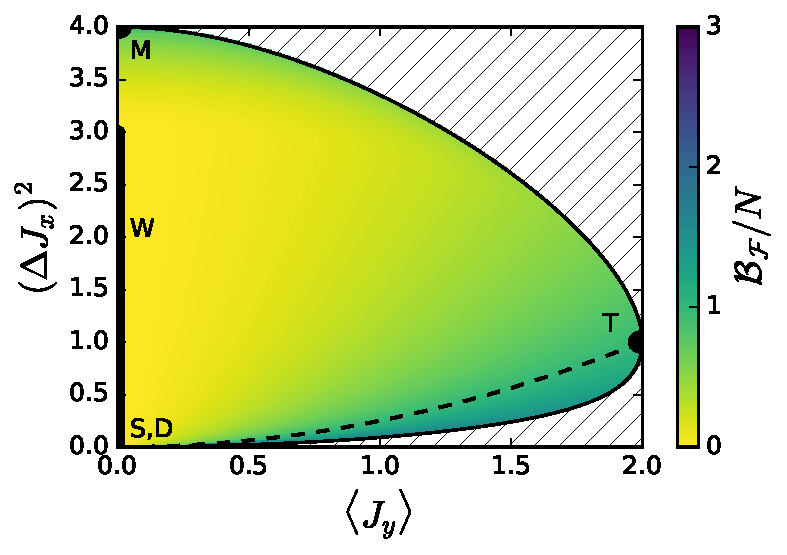
\includegraphics[scale=.65]{img/LT_spsq2d_4.pdf}
  \caption[Solution for 4 particle on the paramenter region for spin-squeezed states.]{We show as a function of the expectation value, $\expect{J_y}$, and the variance in the perpendicular direction, $\varian{J_x}$, the minimum sensitivity for a 4-qubit system.
  (hatched) The physically forbidden region is indicated. (M,T,S,D) Those points indicate where the mixed state (M), the state totally polarized (T), the singlet state (S) and the unpolarized Dicke state (D) would be located. (W) Any of the states from the completely mixed state of the symmetric subspace to the singlet state is in this line. For instance, one can  find the completely mixed state of the whole Hilbert space sitting in that line. (dashed) Shot-noise threshold. Below this line non-classical sensitivities can be achieved.}
  \label{fig:lt-spsq2d-4}
\end{figure}

We now compare the difference between our bound and the bound of L.~Pezze and A.~Smerzi Eq.~\eqref{eq:bg-pezze-bound}.
First, we consider the experimentally relevant region for which $\varian{J_x}\leqslant 1$.
We find that for points away from the physical boundary at least by 0.001 on the vertical axis, the difference between the two bounds is smaller than $2\times10^{-6}$.
Hence, Eq.~\eqref{eq:bg-pezze-bound} practically coincides with the optimal bound for $\varian{J_x}<1$.

For points at the boundary, the difference is somewhat larger, but still small, the relative difference is smaller than $2\%$ for 4 particles.
We compute the difference between the Eq~\eqref{eq:bg-pezze-bound} and our bound for different number of particles and for states at the boundary from the state totally polarized T to the unpolarized Dicke state at D, see Figure~\ref{fig:lt-edge-diff}.
\begin{figure}[htp]
  \centering
  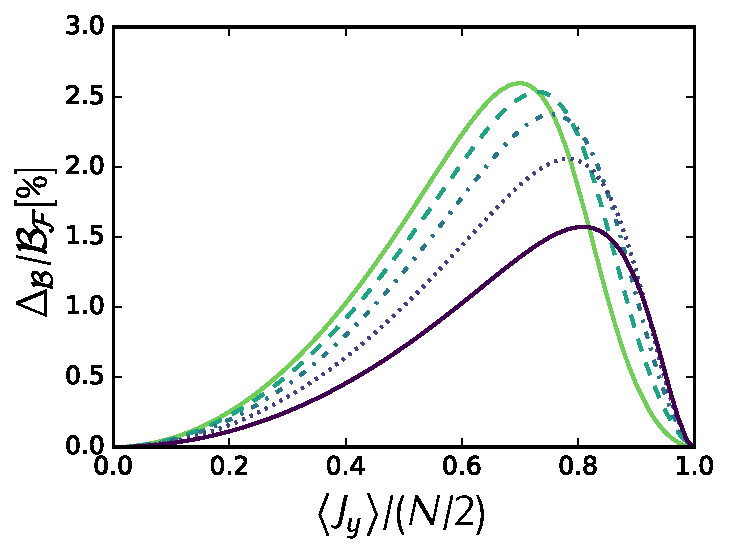
\includegraphics[scale=.65]{img/LT_edge_diff.pdf}
  \caption[Boundary difference of optimal bound versus Pezz\'e-Smerzi bound.]{Difference between the bound of Pezze-Smerzi and the optimal bound for the quantum Fisher information normalized by the value of the optimal bound itself for the bosonic ground states of $H=J_x^2-\lambda J_y$ for $\forall \lambda \in [0,\infty)$.
  From dark to lighter colors (line, point, dash-point, dashed, pointed, line), results for different particle numbers, $N=4,6,10,20,1000$ respectively.
  One can see that for large particle numbers the difference is largest when the polarization is around two thirds of the maximal polarization and that this difference is less than $2.6\%$.}
  \label{fig:lt-edge-diff}
\end{figure}

We now consider regions on Figure~\ref{fig:lt-spsq2d-4} for which $\varian{J_x}>1$.
The difference between the two bound is now larger.
It is larger at point M, for which the bound Eq.~\eqref{eq:bg-pezze-bound} is zero.
Hence for measurement values corresponding to points close to M, our method improve the formula Eq.~\eqref{eq:bg-pezze-bound}.
It is important from the point of view of applying our method to spin-squeezing experiments that the bound Eq.~\eqref{eq:bg-pezze-bound} can be substantially improved for $\varian{J_x}<1$, if we assume bosonic symmetry for the system, or we measure an additional quantity, such as $\expect{J_x^4}$ as shown in Figure~\ref{fig:lt-adding-jx4-to-the-bound} [TD: Ask Geza for data].
\begin{figure}[htp]
  \centering
  % 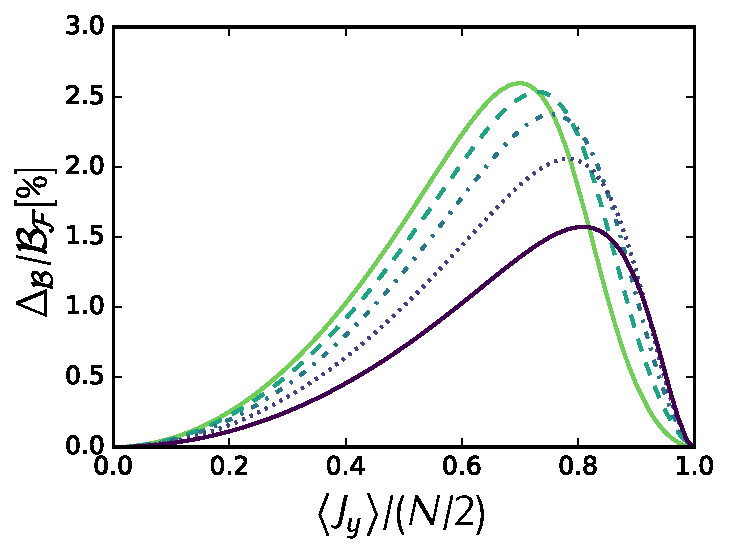
\includegraphics[scale=.65]{img/LT_edge_diff.pdf}
  % \caption[Boundary difference of optimal bound versus Pezz\'e-Smerzi bound.]{Difference between the bound of Pezze-Smerzi and the optimal bound for the quantum Fisher information normalized by the value of the optimal bound itself for the bosonic ground states of $H=J_x^2-\lambda J_y$ for $\forall \lambda \in [0,\infty)$.
  % From dark to lighter colors (line, point, dash-point, dashed, pointed, line), results for different particle numbers, $N=4,6,10,20,1000$ respectively.
  % One can see that for large particle numbers the difference is largest when the polarization is around two thirds of the maximal polarization and that this difference is less than $2.6\%$.}
  \label{fig:lt-adding-jx4-to-the-bound}
\end{figure}


\subsubsection{Dicke states}
\label{sec:lt-bound-dicke-states}

In this section, we use our method to find lower bounds on the QFI for states close to the Dicke states \eqref{eq:vd-unpolarized-dicke} along the $x$-direction, based on collective measurements.
We discuss what operators have to be measured to estimate the metrological usefulness of the state.
In Section~\ref{sec:lt-many-particle-experiments}, we will test our approach for a realistic system with very many particles.

In order to estimate the metrological usefulness of states created in such experiments, we choose to measure $W_1=J_x^2$, $W_2=J_y^2$ and $W_3=J_z^2$ since the expectation values of these operators uniquely define the ideal Dicke state, and they have been already used for entanglement detection \cite{Luecke2014}.
In cold gas experiments of nowadays, the state created is invariant under transformations of the type $U_{x}(\phi)=\exp(-i J_x \phi)$ \cite{Apellaniz2015}.
For such states $\expect{J_y^2}=\expect{J_z^2}$, which we also use as a constraint in our optimization.

Let us demonstrate how our method works in an example for small systems.
Figure~\ref{fig:lt-symmetric-dicke-6-bound}
\begin{figure}[htp]
  \centering
  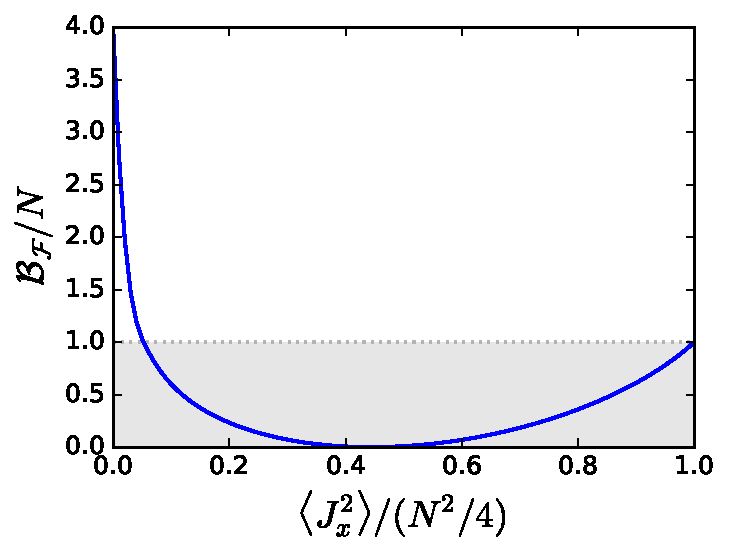
\includegraphics[scale=.65]{img/LT_dicke_edge.pdf}
  \caption[6-particles optimal bound on BEC symmetry for the QFI when $\{\expect{J_x^2},\expect{J_y^2},\expect{J_z^2}\}$ are measured]{Optimal lower bound on the quantum Fisher Information for symmetric states with $\expect{J_y^2}=\expect{J_z^2}$. Even if it is metrologicaly useful for a wide range of $\expect{J_x^2}$, the numerics shows us a tiny region where the metrological gain is surpassing the shot-noise limit.}
  \label{fig:lt-symmetric-dicke-6-bound}
\end{figure}
shows the result for 6 qubits for symmetric states for which
\be
  \label{eq:lt-maximum-angular-momentum}
  \expect{J_x^2+J_y^2+J_z^2} = \frac{N(N+2)}{4}=:\mathcal{J}_N.
\ee
It can be seen that the lower bound on quantum Fisher Information is the largest for $\expect{J_x^2}=0$.
It reaches the value corresponding to the ideal Dicke state, $\qfif{\rho,J_z}/N=(N+2)/2=4$.
It is remarcable that the state is also useful for metrology if $\expect{J_x^2}$ is very large.
In this case $\expect{J_y^2}$ and $\expect{J_z^2}$ are smaller than $\expect{J_x^2}$.

\subsection{Calculations for experimental data}

In this section, we use our method to find tight lower bound on the QFI based on experimental data.
In particular, we will determine the bound for several experiments in photons and trapped ions creating GHZ states and Dicke states, in which the fidelity has been measured \cite{Krischek2011, Zhao2003, Gao2010, Leibfried2004, Sackett2000, Monz2011, Kiesel2007, Wieczorek2009, Prevedel2009, Chiuri2012}, which is much easier than obtaining the quantum Fisher Information from the density matrix \cite{Hyllus2012}, or estimation it from a metrological procedure \cite{Luecke2011}.
We will obtain a bound on the QFI for a spin-squeezing experiment with thousand of particles \cite{Gross2010}.
Based on numerical examples, we see that the bound Eq.~\eqref{eq:bg-pezze-bound} is close to the optimal even for not completely polarized states.
Assuming symmetry or knowing additional expectation values can improve the bound Eq.~\eqref{eq:bg-pezze-bound}.
Finally, we will also obtain the bound for the QFI for a recent experiment with Dicke states \cite{Luecke2014}.
The estimate of the precision based on considering the particular case when $\expect{J_x^2}$ is measured for parameter estimation \cite{Apellaniz2015} is close to the optimal bound computed by our method.

\subsubsection{Few-particle experiments}

Now, we will estimate the quantum Fisher information based on the fidelity with respect to Dicke states and GHZ states for several experiments with photons and trapped cold ions, following the ideas of Section~\ref{sec:lt-bounds-fidelity}.

Our results are summarized in Table~\ref{tab:lt-results-for-fidelities}.
The experiments in \cite{Gao2010,Chiuri2012} are with hyperentangled qubits, while in the rest of experiments a single qubit is stored in a particle.
Ref.~\cite{Monz2011} describes experiments with 2-14 ions, we presented only results of two of them.
Finally, for the experiment of Ref.~\cite{Zhao2004} we used the fidelity estimated using reasonable assumptions discussed in that paper, while the worst case fidelity is lower.
\begin{table}
  \begin{center}
    \begin{tabular}{| l | l | l | l | l |}
      \hline
      Physical&Target &\multicolumn{1}{ l|}{\multirow{2}{*}{Fidelity}}
      &\multicolumn{1}{ l|}{\multirow{2}{*}{$\bound{\mathcal{F}}/N$}}
      &\multicolumn{1}{ l|}{\multirow{2}{*}{Ref.}} \\
      system & quantum state &  &  &  \\ \hline
      \multicolumn{1}{|l|}{\multirow{6}{*}{photons}}
      & \multicolumn{1}{ l|}{\multirow{4}{*}{$\ket{\dicke{4}}$}}
      & $0.844\pm0.008$   & $1.432\pm0.044$ & \cite{Kiesel2007} \\
      & & $0.78\pm0.008$    & $1.124\pm0.236$ & \cite{Chiuri2012} \\
      & & $0.8872\pm0.0055$ & $1.680\pm0.036$ & \cite{Krischek2011} \\
      & & $0.873\pm0.005$   & $1.44\pm0.024$  & \cite{Toth2010} \\ \cline{2-5}
      & \multicolumn{1}{ l|}{\multirow{2}{*}{$\ket{\dicke{6}}$}} &
      $0.654\pm0.024$   & $0.564\pm0.076$ & \cite{Wieczorek2009} \\
      & & $0.56\pm0.02$     & $0.304\pm0.048$ & \cite{Prevedel2009} \\ \hline
      \multicolumn{1}{|l|}{\multirow{5}{*}{photons}}
      & $\ket{\ghz_{4}}$  & $0.840\pm0.007$ & $1.848\pm0.076$ & \cite{Zhao2004} \\
      & $\ket{\ghz_{5}}$  & $0.68$          & $0.65$ & \cite{Zhao2004} \\
      & $\ket{\ghz_{8}}$  & $0.59\pm0.02$   & $0.256\pm0.128$ & \cite{Huang2011} \\
      & $\ket{\ghz_{8}}$  & $0.776\pm0.06$  & $2.4376\pm0.1072$ & \cite{Gao2010} \\
      & $\ket{\ghz_{10}}$ & $0.561\pm0.019$ & $0.15\pm0.11$ & \cite{Gao2010} \\ \hline
      \multicolumn{1}{|l|}{\multirow{5}{*}{trapped-ions}}
      & $\ket{\ghz_{3}}$  & $0.89\pm0.03$   & $1.824\pm0.291$ & \cite{Leibfried2004} \\
      & $\ket{\ghz_{4}}$  & $0.57\pm0.02$   & $0.08\pm0.052$  & \cite{Sackett2000}\\
      & $\ket{\ghz_{6}}$  & $0.509\pm0.004$ & $0.0018\pm0.0018$ & \cite{Leibfried2005} \\
      & $\ket{\ghz_{8}}$  & $0.817\pm0.004$ & $3.21\pm0.08$ & \cite{Monz2011} \\
      & $\ket{\ghz_{10}}$ & $0.626\pm0.006$ & $0.64\pm0.06$ & \cite{Monz2011} \\ \hline
    \end{tabular}
  \end{center}
  \caption[Bounds on QFI for experimental data when fidelities are measured]{Fidelity values and the corresponding bound for the QFI for several experiments with Dicke states and GHZ states.
  Bounds normalized with $N$ are shown.
  The ones surpassing the value one in the fourth column show quantum entanglement enhanced metrological usefulness.
  For Dicke states the maximum is achieved at $(N+2)/2$, i.e., $3$ for the $\ket{\dicke{4}}$ case and $4$ for the $\ket{\dicke{6}}$ case.
  For the case in which GHZ states are used the limit for the normalized bound is $N$, the particle number.}
  \label{tab:lt-results-for-fidelities}
\end{table}

We can compare our estimate to the quantum Fisher information of the state for the experiment of Ref.~\cite{Krischek2011}, where the QFI for the density matrix was obtained as $\qfif{\rho,J_z}/N=(10.326\pm0.093)/N=(2.5816\pm0.02325)$.
As can be seen in Table~\ref{tab:lt-results-for-fidelities}, this value is larger than we obtained, however, it was calculated by knowing the entire matrixm, while our bound is obtained from the fidelity alone.

\subsubsection{Many-particle experiments}
\label{sec:lt-many-particle-experiments}

In this section, we will estimate the quantum Fisher information based on collective measurements for experiments aiming to create spin-squeezing states and Dicke states.

\subsubsubsection{Spin-squeezing experiment}

We turn our attention to a recent many-particle spin-squeezing experiment in cold gases to use our method to find lower bounds on the quantum Fisher information, following the ideas of Section~\ref{sec:lt-bound-spsq}.
With that we show that the lower bound given in Eq.~\eqref{eq:bg-pezze-bound} is close to the optimal.
We also demonstrate that we carry out calculations for real systems.

In particular, for our calculations we use the data from spin-squeezing experiments of Ref.~\cite{Gross2010}.
The particle number is $N=2300$, and the spin squeezing parameter defined as
\be
  \label{eq:lt-spin-squeezing-parameter}
  \xi_{\textnormal{s}}^2 = N \frac{\varian{J_x}}{\expect{J_y}^2}
\ee
has the value $\xi_{\textnormal{s}}^2=-8.2\db=10^{-8.2/10}=0.1514$.
The spin length $\expect{J_y}$ has been close to maximal.
In our calculations, we choose
\be
  \expect{J_y}=\alpha \frac{N}{2},
\ee
where we will test our method with various values for $\alpha$.
For each $\alpha$ we use $\varian{J_x}$ will be given such that we get the experimentally obtained spin-squeezing parameter Eq.~\eqref{eq:lt-spin-squeezing-parameter}.
Moreover, we assume $\expect{J_x}=0$, as the $y$-direction was the direction of the mean spin in the experiment.
Based on Eq.~\eqref{eq:bg-pezze-bound}, the bound for the quantum Fisher information is obtained as
\be
  \label{eq:lt-bound-for-experiment}
  \frac{\qfif{\rho,J_z}}{N}\geqslant \frac{1}{\xi_{\textnormal{s}}^2}=6.605.
\ee

For our computations we need a tool to handle large systems.
We will carry out the calculations for symmetric states.
this way we obtain a lower bound on the QFI that we will denote by $\bound{\textnormal{sym}}$.
As already mentioned, we could obtain a bound for the QFI that is valid even for general case, not necessarily symmetric states if the matrix from which compute the maximum eigenvalue Eq.~\eqref{eq:lt-legendre-for-qfi-simplified} has a non-degenerated largest eigenvalue.
This is not the case in general for the spin-squeezing problem.
However, we still know that our bound obtained with our calculations in the symmetric subspace cannot be smaller than the optimal bound $\bound{\mathcal{F}}$, which must be larger or equal to the Eq.~\eqref{eq:bg-pezze-bound} since it cannot be smaller than the optimal bound for general states.
These relations can be summarized as
\be
  \bound{\textnormal{sym}}\geqslant \bound{\mathcal{F}}\geqslant\frac{\expect{J_y}^2}{\varian{J_x}},
\ee
where on the right-hand side we just used the bound in Eq.~\eqref{eq:bg-pezze-bound}.

Our calculations lead to
\be
  \label{eq:lt-symmetric-optimal-pezze-inequality}
  \frac{\bound{\textnormal{sym}}(\expect{J_y},\varian{J_x})}{N} = 6.605
\ee
for a wide range of values of $\alpha$.
That is, based on numerics, the left-hand side and the right-hand side of Eq.~\eqref{eq:lt-symmetric-optimal-pezze-inequality} seem to be equal.
This implies that the lower bound Eq.~\eqref{eq:bg-pezze-bound} is optimal for estimating the QFI for the system.

We follow giving the details of our calculations for $\alpha=0.5,0.85$ and we show examples in which we can improve the bound Eq.~\eqref{eq:bg-pezze-bound} with our approach, if symmetry is assumed.
We present simple scheme that we need to handle large systems, and make calculations for larger particle number.
Thus, we need fewer steps for the numerical optimization for large system sizes, which makes our computations faster.
Second, while we will be able to carry out the calculation for the particle number of the experiment, we will also see that we could even extrapolate the results from the results obtained for lower particle numbers.
This is useful for future application of our method for very large systems.

The basic idea is that we transform the collective quantities from $N$ to a smaller particle number using the scaling relation
\begin{align}
  \expect{J_y} & = \frac{N'}{2}\alpha,\\
  \varian{J_x} & = \xi_{\textnormal{s}}^2 \frac{N'}{4}\alpha^2.
\end{align}
We see that for the scaling we consider, for all $N'$ the bound in Eq.~\eqref{eq:bg-pezze-bound} is valid, i.e., is obtained as
\be
  \frac{\qfif{\rho_{N'},J_z}}{N'}\geqslant \frac{1}{\xi_{\textnormal{s}}^2}=6.605.
\ee

Let us first take $\alpha=0.85$, which is somewhat smaller than the experimental value, however, it helps us to see various characteristics of the method.
At the end of the section we will also discuss the results for other values of $\alpha$.
Based on these ideas, we compute the bound $\bound{\textnormal{sym}}$ for the quantum Fisher information for an increasing system size $N'$.

The results can be seen in Figure~\ref{fig:lt-bounds-on-symmetric-spin-squeezing}.a.
\begin{figure}[htp]
  \centering
  \igwithlabel{(a)}{scale=.65}{img/LT_spsq_scaling_1.pdf}
  \igwithlabel{(b)}{scale=.65}{img/LT_spsq_scaling_2.pdf}
  \caption[Asymptotic behavior of the bound for increasing particle number for spin-squeezing experimental data]{[TD: Change vertical label to $\bound{\textnormal{sym}}$] (Color line) Lower bound on the QFI based on $\expect{J_y}$ and $\varian{J_x}$ obtained for the symmetric subspace for different particle numbers $N'$.}
  \label{fig:lt-bounds-on-symmetric-spin-squeezing}
\end{figure}
The bound obtained this way is close to the bound in Eq.~\eqref{eq:lt-bound-for-experiment} even for small $N'$.
For larger particle number it is constant and coincides with the bound in Eq.~\eqref{eq:lt-bound-for-experiment}
This also strongly supports the idea that we could used the result for small particle numbers to extrapolate the bound for $N$.
Since for the experimental particle number we obtain that $\bound{\text{sym}}$ equals the bound in Eq.~\eqref{eq:lt-bound-for-experiment}, we find that all three lower bounds in Eq.~\eqref{eq:lt-symmetric-optimal-pezze-inequality} must be equal.
Hence, Eq.~\eqref{eq:bg-pezze-bound} is optimal for the experimental system and $\alpha$ considered before in this section.
Besides, these results present also a strong argument for the correctness of our approach.

We now give more details of the calculation. We were able to carry out the optimizations up to $N'=2300$ with a usual laptop computer using MATLAB programming language\footnote{
For MATLAB R2015a, see \url{http://www.mathworks.com}.}.
We started the calculation for each given particle number with the $r_k$ parameters obtained for the previous simulation with a smaller particle number.
This allows for faster finding of the solution than if we would start the $r_k$ parameters arbitrarily.

Let us consider a spin-squeezing state that is not fully polarized and $\alpha=0.5$.
In Figure~\ref{fig:lt-bounds-on-symmetric-spin-squeezing}.b, we can see that for small particle numbers we have a larger bound on $\qfif{\rho, J_z}$ than the one obtained from Eq~\eqref{eq:bg-pezze-bound}.
Thus for the case in which the particle number would be smaller we could improve the bound Eq.~\eqref{eq:bg-pezze-bound} by assuming symmetry.
On the other hand, for large particle number we recover the bound Eq.~\eqref{eq:bg-pezze-bound}.

Finally, we add a note on the technical details.
We carried out our calculations with the constraints on $\varian{J_x}$ and $\expect{J_y}$, with the additional constraint $\expect{J_x}=0$.
For the experimental particle numbers, one can show that our results are valid even if we constrained only $\varian{J_x}$ and $\expect{J_y}$, and did not use the $\expect{J_x}=0$ constraint.
This way, in principle, we could only get a lower bound that is equal to the one we obtained before or lower.
However, we obtained before a value identical to the analytical bound Eq.~\eqref{eq:bg-pezze-bound}.
The optimal bound cannot be below the analytic bound, since then the analytic bound would overestimate the quantum Fisher information, and it would not be a valid bound.
Hence, even an optimization without the $\expect{J_x}=0$ constraint could not obtain a smaller value than our results.

\subsubsubsection{Experiment creating Dicke states}

In this section, we present our calculations for an experiment aiming at creating Dicke states in cold gases \cite{Luecke2014}.
The basic ideas are similar to the ones explained in Section~\ref{sec:lt-bound-dicke-states} for small systems.
The experimental data, as in previous Section~\ref{sec:vd-testing-with-experimental-data}, are $N=7900$, $\expect{J_y^2}=112\pm31$, $\expect{J_x^2}=\expect{J_z^2}=6\times10^6\pm0.6\times10^6$ \cite{Apellaniz2015}.
Applying some simple transformations, we can make calculations for a very large numbers of particles, and obtain results even for general, non-symmetric systems.

In the general, non-symmetric case, we can handle only small problems.
Thus, we have to transform the collective quantities such that the corresponding quantum state, i.e., it has to fulfill
\be
  \expect{J_x^2}_{\text{sym}} + \expect{J_x^2}_{\text{sym}} + \expect{J_x^2}_{\text{sym}} = \mathcal{J}_N,
\ee
where $\mathcal{J}_{N}$ is defined on Eq.~\eqref{eq:lt-maximum-angular-momentum}.
A mapping of this type can be realized equally scaling all second moments of the angular momentum projections as
\be
  \label{eq:lt-expectation-values-extended-to-symmetric}
  \expect{J_l^2}_{\text{sym}, N} = \gamma \expect{J_l^2}_N,
\ee
where we now added the label $N$ to avoid confusions in upcoming equations, $l=x,y,z$ and where we used the coefficient $\gamma$ to be
\be
  \label{eq:lt-value-of-gamma}
  \gamma = \frac{\mathcal{J}_N}{\expect{J_x^2}_N +\expect{J_y^2}_N +\expect{J_z^2}_N}.
\ee
Note that $\gamma=1$ if the original state is symmetric.

Next, based on the ideas of this chapter, we calculate the lower bound on the quantum Fisher information for symmetric systems, which we denote it by $\bound{\text{sym},N}$.
Then, to obtain the results for the original non-symmetric case, note the convex nature of the $\bound{N}$, which is the bound to be computed for the general case, implies
\be
  \bound{N}\leqslant \frac{1}{N}\bound{\text{sym},N},
\ee
where $\bound{\text{sym},N}$ corresponds to the bound one would obtain in the symmetric subspace for expectation values given using the Eq.~\eqref{eq:lt-expectation-values-extended-to-symmetric}.
This can be seen using an auxiliary state $\tilde{\rho}$ that mixes the symmetric state that in principle has the expectation values appearing in Eq.~\eqref{eq:lt-expectation-values-extended-to-symmetric} and the singlet state that has zero value for all those expectation values
Hence, if we construct a mixture of this type as follows
\be
  \tilde{\rho}_N=(1-\gamma^{-1}) \rho_{\text{singlet},N}+\gamma^{-1}\rho_{\text{sym},N},
\ee
we have that $\tilde{\rho}$ has the same expectation values as the original non-symmetric case.
This way, we can relate the bound for general systems to the quantum Fisher information for symmetric cases as
\be
  \label{eq:lt-radial-linearity-dicke-bound}
  \bound{N}\leqslant \qfif{\tilde{\rho}_N,J_z}=\frac{1}{\gamma}\qfif{\rho_{\text{sym,N}},J_z}.
\ee
Here, the inequality comes due to that our bound cannot be larger than the QFI of any state having the given set of expectation values.
On the other hand, the equality holds due to the fact that both $\tilde{\rho}$ and $J_z$ can be written as block-diagonal matrix of blocks corresponding to different eigenvalues of $\bs{J}^2$.
In particular, $\rho_{\text{singlet},N}$ has non-zero elements only in the blocks for which $\expect{\bs{J}^2}=0$, while $\rho_{\text{sym},N}$ has nonzero elements only in the blocks in which $\expect{\bs{J}^2}$ is maximal.
Note that $\bs{J}^2$ is a shorthand of $J_x^2+J_y^2+J_z^2$.
Then we can use the general formula \cite{Toth2014}
\be
  \qfif{\bigoplus_k p_k\rho_k, \bigoplus_k A_k}= \sum_k p_k \qfif{\rho_k,A_k},
\ee
where $\rho_k$ are density matrices with unit trace, $\sum_k p_k=1$ and the $k$ index represent the block subspaces of the system and the operators $A_k$.

Extensive numerics for small systems show that the inequality in Eq.~\eqref{eq:lt-radial-linearity-dicke-bound} is very close to an equality within the numerical precision
\be
  \label{eq:lt-bound-extrapolation-from-symmetric-dicke}
  \bound{N}\approx\frac{1}{\gamma}\bound{\text{sym},N}.
\ee
To obtain the lower bound $\bound{N}$ we also use an increasing system size $N'$ as we have done in at the beginning of this section.
However, in this case we will not be able to do the calculation for the experimental particle number, and we will use extrapolation from the results obtained for smaller particle numbers.

First, we transform the measured second moments to values corresponding to a symmetric system using Eqs.~\eqref{eq:lt-expectation-values-extended-to-symmetric} and \eqref{eq:lt-value-of-gamma}.
For our case, $\gamma=1.301$.
This way, we obtain
\be
  \begin{split}
    \expect{J_y^2}_{\text{sym},N}&=145.69,\\
    \expect{J_x^2}_{\text{sym},N}&=\expect{J_z^2}_{\text{sym},N}=7.8\times10^6.
  \end{split}
\ee

Next, we will carry out calculations for symmetric systems.
We will consider a smaller system $N'$ that keeps expectation values such that the corresponding quantum state must be symmetric.
Hence, we will use the following relation to find the target expectation values for smaller systems
\be
  \begin{split}
    \expect{J_y^2}_{\text{sym},N'}&=\expect{J_y^2}_{\text{sym},N},\\
    \expect{J_x^2}_{\text{sym},N'}&=\expect{J_z^2}_{\text{sym},N'} =\frac{1}{2}(\mathcal{J}_{N'})-\expect{J_y^2}_{\text{sym},N'}),
  \end{split}
\ee
where $\mathcal{J}_{N'}$ is defined in Eq.~\eqref{eq:lt-maximum-angular-momentum}.
Note that with Eq.~\eqref{eq:lt-maximum-angular-momentum} holds for all $N'$, hence the state must be symmetric.
Hence, the main characteristics of the scaling relation can be summarized as follows, $\expect{J_y^2}_{\text{sym},N'}$ remains equal for all $N'$ while $\expect{J_x^2}_{\text{sym},N'}$ and $\expect{J_z^2}_{\text{sym},N'}$ are chosen such that they are equal to each other and the state is symmetric.
For large N, this implies a scaling of $\expect{J_y^2}_{\text{sym},N}$ constant and $\expect{J_x^2}_{\text{sym},N}=\expect{J_z^2}_{\text{sym},N}\sim N(N+2)/8$.

Let us now turn to central quantities of our chapter, the lower bounds on the quantum Fisher information.
A central point in our scheme is that due to the scaling properties of the system, we can obtain the value for the particle number $N$ from the values of a smaller particle number $N'$ as \cite{Zhang2014}
\be
  \label{eq:lt-asymptotic-limit-bound-dicke-symmetric}
  \bound{\text{sym},N}\approx\frac{\mathcal{J}_{N}}{\mathcal{J}_{N'}} \bound{\text{sym},N'},
\ee
which we will verify numerically.
Note that for large $N$, we have $\mathcal{J}_{N}/\mathcal{J}_{N'}\sim N^2/(N')^2$.

As last step, we have to return from the symmetric system to our real system, not fully symmetric one.
Based on Eq.~\eqref{eq:lt-asymptotic-limit-bound-dicke-symmetric} and assuming Eq.~\eqref{eq:lt-bound-extrapolation-from-symmetric-dicke}, a relation for the lower bound for the original problem can be obtained from the bound on the symmetric problem with $N'$ particles as
\be
  \label{eq:lt-definitive-formula-scaling-dicke}
  \bound{N}\approx \frac{1}{\gamma}\frac{\mathcal{J}_{N}}{\mathcal{J}_{N'}} \bound{\text{sym},N'} =\frac{\expect{J_x^2}_N+\expect{J_y^2}_N+\expect{J_z^2}_N}{\mathcal{J}_N'}\bound{\text{sym},N'}.
\ee
In Figure~\ref{fig:assimpthotic-approach-to-the-bound-from-scaled-dicke},
\begin{figure}[htp]
  \centering
  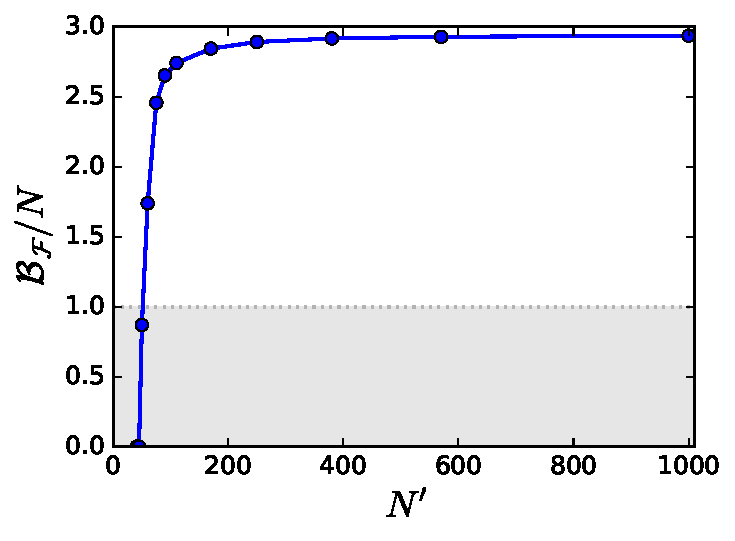
\includegraphics[scale=.65]{img/LT_dicke_7900_asymp.pdf}
  \caption[Asymptotic behaviour of the bound for increasing size systems for Dicke like experimental data]{Secuence of the evolution of an unpolarized Dicke state of 16 qubits for $\theta=\{i\pi/6\}_{i=0}^4$. Bloch spheres representing the Hirusi distribution of the state, and below PDF of the $J_x$ POVM for each step of the secuence}
  \label{fig:assimpthotic-approach-to-the-bound-from-scaled-dicke}
\end{figure}
we plotted the right-hand side of Eq.~\eqref{eq:lt-definitive-formula-scaling-dicke} as the function of $N'$ divided by $N$.
We can see that $\bound{N'}/N$ is constant or slightly increasing for $N'>400$.
This is a strong evidence that Eq.~\eqref{eq:lt-asymptotic-limit-bound-dicke-symmetric} is valid for relatively large particle numbers.
With this, we arrive at the result for the experimental system
\be
  \label{eq:lt-result-experimental-dicke}
  \frac{\bound{N}(\expect{J_y^2},\expect{J_x^2}=\expect{J_z^2})}{N}\approx 2.94.
\ee
The $\approx$ sign is used referring to the fact that we assume that the inequality in Eq.~\eqref{eq:lt-radial-linearity-dicke-bound} is close to be saturated and that we did sufficient numerics for an increasing system size $N'$ to have a good asymptotic approach to the real value Eq.~\eqref{eq:lt-asymptotic-limit-bound-dicke-symmetric}.

It is instructive to compare the value of Eq.~\eqref{eq:lt-result-experimental-dicke} to the one obtained in Section~\ref{sec:vd-testing-with-experimental-data}, where the same system was characterized base on its metrological usefulness.
Such result implies $\qfif{\rho,J_z}/N\geqslant3.3$ which is somewhat bigger than our recent result as we did not use the knowledge of the fourth moments, only the second moments.
The closeness of the two results is a strong argument for the correctness of our calculations.

\subsection{Scaling for $\qfif{\rho,J_z}$ with $N$}

Recent important works examine the scaling of the quantum Fisher information with the particle number for metrology under the presence of decoherence \cite{Escher2011, Demkowicz-Dobrzanski2012}.
They consider the QFI defined now for the non-unitary, noisy evolution.
They find that for small $N$ it is close to the value obtained by considering coherent dynamics.
Hence, even the Heisenberg scaling, $\mathcal{O}(N^2)$, can be reached.
However, if $N$ is sufficiently large, then, due to the decoherence during the parameter estimation, the QFI scales as $\mathcal{O}(N)$.

We have to stress that the findings of \cite{Escher2011, Demkowicz-Dobrzanski2012} are not applicable to our case.
Our methods estimates the quantum Fisher information assuming a perfect unitary dynamics.
The quantum Fisher information can be smaller that what we expect ideally only due to the imperfect preparation of the state\footnote{
This is also relevant for \cite{Augusiak2015}, where $\qfi=\mathcal{O}(N^2)$ is reached with weakly entangled states.}.
We can even find simple conditions on the state preparation that lead to a Heisenberg scaling.
Based on Eq.~\eqref{eq:lt-ghz-legendre-solution}, if we could realize quantum states $\rho_N$ such that $F_{\text{GHZ}}(\rho_N)\geqslant0.5+\epsilon$ for $N\rightarrow\infty$ for some $\epsilon>0$, then we would reach $\bound{\mathcal{F}}(F_{\text{GHZ}}) = \mathcal{O}(N^2)$.
Strong numerical evidence suggest that a similar relation holds for fidelity $F_{\text{Dicke}}$ and $\bound{\mathcal{F}}(F_{\text{GHZ}})$, see Section~\ref{sec:lt-bound-dicke-states}.
[TD: Decide if remove the following sentence. It is very strong]
From another point of view, our method can estimate $\qfif{\rho,J_z}$ for large particle numbers, while a direct measurement of the metrological sensitivity considerably underestimates it.


%%%%%%%%%%%%%%%%%%%%%%%%
\section[Metrology of the gradient magnetic field]
{Accuracy bound for gradient field estimation with atomic ensembles}
\thiswatermark{\put(1,-282){\color{l-grey}\rule{84pt}{88pt}}
\put(84,-282){\color{grey}\rule{410pt}{88pt}}}



\section[Metrology of the gradient magnetic field]
{Accuracy bound for gradient field estimation with atomic ensembles}
\label{sec:gm}
\thiswatermark{\put(1,-282){\color{l-grey}\rule{84pt}{88pt}}
\put(84,-282){\color{grey}\rule{410pt}{88pt}}}


\quotes{Ronald Fisher}{To consult the statistician after an experiment is finished is often merely to ask him to conduct a post mortem examination. He can perhaps say what the experiment died of.}

\lettrine[lines=2, findent=3pt, nindent=0pt]{I}{n} this chapter, one of the most fundamental two-parameter estimation tasks in magnetometry is considered, namely gradient magnetometry.
We will add the gradient of the magnetic field as the second parameter beside the constant (homogeneous) part of the field.
While most works in magnetometry with a single ensemble focus only on the determination of the strength and direction of magnetic field, certain measurement schemes for the gradient have already been proposed and tested experimentally.
We study gradient magnetometry with an ensemble of atoms described by a very general probability distribution function for the position of the atoms, and considering atoms with an arbitrary spin.
Some schemes use an imaging of the ensemble with a high spatial resolution, however, they do not count as single-ensemble methods in the sense we use this expression in our paper, since in this case not only collective observables are measured  \cite{Vengalattore2007,Zhou2010,Koschorreck2011}.
There is a method based on collective measurements of the spin length of a fully polarized ensemble \cite{Behbood2013}.
Finally, there is a scheme where they use as a trial state a many-body singlet states, which is described in Ref.~\cite{Urizar-Lanz2013}.

We calculate precision bounds for estimating the gradient of the magnetic field based on the quantum Fisher information.
For quantum states that are invariant under the homogeneous magnetic field, a single parameter estimation is sufficient.
In contrast to this, for states that are sensitive to the homogeneous fields, a two-parameter estimation problem must be solved to obtain the gradient parameter, since the homogeneous field must be also taken into account.
We use our method to calculate precision bounds for gradient estimation with a chain of atoms and even with two spatially separated atomic ensembles which feel different magnetic fields.
As we said, we also consider a single atomic ensemble with an arbitrary density profile, in which atoms cannot be addressed individually, which is a very relevant case for experiments.
Our model can take into account even correlations between particle positions.

The atoms will be distributed along the $x$-axis, so $y=z=0$, and in principle they will be able to feel differences in the magnetic field at different points of the axis.
The magnetic field at the atoms will be given by a linear function of the position $x$
\begin{equation}
\bs{B}(x,0,0)=\bs{B}_0 +x \bs{B}_1 + O(x^2),
\end{equation}
where we will neglect the terms of order two or higher.
We will consider the magnetic field pointing along the $z$-direction direction only, $\bs{B}_0=B_0 \bs{k}$ and $\bs{B}_1=B_1\bs{k}$, where $\bs{k}$ is the unitary vector pointing on the $z$-direction.
For this configuration, due to the Maxwell equations, with no currents or changing electric fields, we have
\begin{align}
\nabla \cdotp \bs{B}&=0, \nonumber \\
\nabla \times \bs{B}&=\bs{0},
\end{align}
where $\bs{0}\equiv (0,0,0)$ is the 3-dimensional null vector.
This implies $\sum_{l=x,y,z} \partial_l B_l=0$ and $ \partial_m B_l - \partial_l B_m =0$ for all $l\ne m$, where $\partial_m\equiv \partial/\partial_m$ stands for the partial derivative over the variable $m$.
Thus, the spatial derivatives of the field components are not independent of each other.
However, in the case of a linear arranged particle ensemble only the derivative along the $x$-axis has an influence on the quantum dynamics of the atoms.

We will determine the precision bounds for the estimation of the magnetic field gradient $B_1$ based on the quantum Fisher information \cite{Paris2009,Braunstein1994,Holevo1982,Helstrom1976,Petz2002,Petz2008}.
In this context the Heisenberg and shot-noise scaling are defined as usual.
The achievable precision in terms of the number of particles scale as $\varinv{\theta}\sim N$ and $\varinv{\theta}\sim N^2$ for SNS and HS respectively.
We will show that with spin chains or two ensembles at different positions the Heisenberg scaling is possible.
Concerning the case of a single ensemble, we will show the following.
Since in such systems the atoms cannot be be individually addressed, we will assume that the quantum state is permutationally invariant.
We will show that for states insensitive to the homogeneous magnetic field, one can reduce the problem to a one-parameter estimation scenario.
Such states can arise in a single-ensemble scheme, however, it will be shown that the Heisenberg limit cannot be reached in this case.
When the state is sensitive to the homogeneous field, the spatial correlation between the atoms must be taken into account in order to show whether the system can overcome the shot-noise scaling and achieve the Heisenberg scaling.
Nevertheless, single-ensemble measurements have certain advantages since the spatial resolution can be higher and the experimental requirements are smaller since only a single ensemble must be prepared.

On the other hand, for states sensitive to the homogeneous field, the classical limit can be overcome only if the particle positions are highly correlated with each other.
Our calculations are generally valid for any measurement, thus they are relevant to many recent experiments \cite{Wasilewski2010,Eckert2006,Wildermuth2006, Wolfgramm2010,Koschorreck2011,Vengalattore2007,Zhou2010,Behbood2013}.
We note that in the case of the singlet, our precision bounds are saturated by the metrological scheme presented in Ref.~\cite{Urizar-Lanz2013}.

We can also connect our results to entanglement theory \cite{Werner1989,Horodecki2009,Guehne2009}.
We find that even in the case of gradient magnetometry the shot-noise scaling cannot be surpassed with separable states, while the Heisenberg scaling can be reached with entangled states.
However, in the single-ensemble scenario, the shot-noise scaling can be surpassed only if the particle positions are correlated, which is the case if the particles attract each other.
We will go into the details in Section~\ref{sec:gm-single-cloud}.

The following sections are organized as follows. In Section~\ref{sec:gm-the-setup}, we will present the setup of the system.
In Section~\ref{sec:gm-cramer-rao-bounds}, the metrological basic concepts used in the chapter are presented.
In Section~\ref{sec:gm-io-chain-and-two-ensembles}, we will show the results for the chain of ions and for when two distant ensembles are considered
In Section~\ref{sec:gm-single-cloud}, we restrict our calculations to single PI atomic ensembles and we develop some particular cases, such as the singlet spin state or the totally polarized state.

\subsection{The setup}
\label{sec:gm-the-setup}

In this section, we will present characteristics of our setup.
For simplicity, as well as following  recent experiments (e.g., Ref.~\cite{Koschorreck2011}), we will consider an ensemble of spin-$j$ particles placed in a one-dimensional setup, $x$ being the spatial coordinate.
Furthermore, we assume that the particles are point-like particles, which is a good approximation when the wave-packet of each particle is much smaller than the trap in which they are or the size of the trap is much smaller than the, let us say, the distance between two traps of a differential metrology device.
We also assume that we have particles that behave classically among each other, i.e., that there is a negligible probability of been two particles in the same spot or that their wave-functions overlap.
Hence, we can treat them as distinguishable particles for all purposes.
On the other hand, they have internal degrees of freedom, their spin, that is quantum. This is a very good description to many of the cold gas experiments.

Based on these considerations, we assume that the state is factorizable into a spatial and a spin part as
\be
\label{eq:gm-separated-internal-and-external}
\rho=\rho^{(\text{x})}\otimes\rho^{(\text{s})},
\ee
and that the spatial part can be characterized as an incoherent mixture of point-like particles that can be written as
\be
  \rho^{(\text{x})}=\int \prob(\bs{x}) \ketbra{\varphi_{\bs{x}}}{\varphi_{\bs{x}}}\,\text{d}^N\bs{x}.
  \label{eq:gm-pre-thermal-state}
\ee
where $\ket{\varphi_{\bs{x}}}$ is a pure state of each particle been placed at $\bs{x}=(x_1,x_2,\dots,x_N)$, respectively.
Each part of the state acts on different Hilbert spaces denoted by $\mathcal{H}^{(\text{x})}$ and $\mathcal{H}^{(\text{s})}$, respectively.
Note that we skip to write the superscript $(\text{x})$, denoting the Hilbert space at which $\ket{\varphi_{\bs{x}}}$ belongs, for simplicity.

In order to write the operators, including the state $\rho^{(\text{x})}$, acting on the Hilbert space $\mathcal{H}^{(\text{x})}$, we will invoke the completeness relation found on the literature \citep{Sakurai2010, Cohen-Tannoudji1977} for the spatial continuous Hilbert space
\be
  \int \ketbra{\bs{x}}{\bs{x}}\,\text{d}^N\bs{x} = \mtxid,
\ee
where $\ket{\bs{x}}=\ket{x_1}^{(1,\text{x})}\otimes\ket{x_2}^{(2,\text{x})}\cdots\otimes\ket{x_N}^{(N,\text{x})}$ is the tensor product of the position eigenvectors of each particle which obey
\be
  \braket{\bs{x}}{\bs{y}} = \delta(\bs{x}-\bs{y}),
\ee
where $\delta(\bs{x}-\bs{y})$ is the Dirac delta found in the literature \citep{Sakurai2010, Cohen-Tannoudji1977}.

To see how our notation works, let us write the vector of the position operators for each particle as $\hat{\bs{x}}\equiv(x^{(1)},x^{(2)},\dots,x^{(N)})$, where we used the "$\hat{}$" notation to distinguish it from the vector of position variables.
It is known that $\hat{\bs{x}}$ acting on $\ket{\bs{x}}$ will give $\bs{x}\ket{\bs{x}}$ \cite{Sakurai2010, Cohen-Tannoudji1977}.
Hence,
\be
  \hat{\bs{x}} = \hat{\bs{x}}\mtxid = \hat{\bs{x}} \int \ketbra{\bs{x}}{\bs{x}}\,\text{d}^N\bs{x} = \int \hat{\bs{x}} \ketbra{\bs{x}}{\bs{x}}\,\text{d}^N\bs{x} = \int \bs{x} \ketbra{\bs{x}}{\bs{x}}\,\text{d}^N\bs{x}.
\ee
We can follow similar arguments to rewrite the pure state $\ket{\varphi_{\bs{x}}}$.
First, note also that the expectation value of the position operator for such a state is always $\bs{x}$.
Hence, such a state must be proportional to $\ket{\bs{x}}$.
On the other hand, a pure state must be normalized to one, hence, we can construct such a state by dividing the eigenvector $\ket{\bs{x}}$ by the square-root of its norm as
\be
  \ket{\varphi_{\bs{x}}} \equiv \frac{\ket{\bs{x}}}{\sqrt{\braket{\bs{x}}{\bs{x}}}}.
\ee
For illustrative purposes, we compute in this basis the expectation value of the position operator for these pure states as
\be
  \expect{\hat{\bs{x}}}_{\varphi_{\bs{x}}} = \braopket{\varphi_{\bs{x}}}{\int \bs{y} \ketbra{\bs{y}}{\bs{y}}\,\text{d}^N\bs{y}}{\varphi_{\bs{x}}} =
  \int \bs{y}
  \frac{\braket{\bs{x}}{\bs{y}}\braket{\bs{y}}{\bs{x}}}
  {\braket{\bs{x}}{\bs{x}}} \,\text{d}^N\bs{y} =
  \bs{x}\frac{\braket{\bs{x}}{\bs{x}}}{\braket{\bs{x}}{\bs{x}}} =
  \bs{x},
\ee
where in the step before the last we have used $\braket{\bs{y}}{\bs{x}}=\delta(\bs{y}-\bs{x})$ to compute the integral.
Using that $\braket{\bs{x}}{\bs{x}}=\delta(\bs{0})$, where $\bs{0}$ is a $N$-dimensional vector of zeros, we can rewrite the spatial state Eq.~\eqref{eq:gm-pre-thermal-state} as
\be
  \rho^{(\text{x})}=\int \frac{\prob(\bs{x})}{\delta(\bs{0})} \ketbra{\bs{x}}{\bs{x}}\,\text{d}^N\bs{x}.
  \label{eq:gm-thermal-state}
\ee
Note also that if the eigen-decomposition of the internal state is $\rho^{(\text{s})} = \sum_{\lambda} p_{\lambda}\ketbra{\lambda}{\lambda}$, then the whole state is decomposed as
\be
  \rho = \int\sum_{\lambda} \frac{\prob(\bs{x})}{\delta(\bs{0})} p_\lambda \ketbra{\bs{x},\lambda}{\bs{x},\lambda}\,\text{d}^N\bs{x},
  \label{eq:gm-eigendecomposition-of-state}
\ee
where $\ket{\bs{x},\lambda}$ is a shorthand for $\ket{\bs{x}}^{(\text{x})}\otimes\ket{\lambda}^{(\text{s})}$, the eigenstates, where their corresponding eigenvalues are in this case $\frac{\prob(\bs{x})}{\delta(\bs{0})} p_\lambda$.

At this point, we want to emphasize that our method could easily be extended to the case of Bose-Einstein condensates, or any other spatial configuration, not considered in this paper. In the case of BECs, the spatial state of the particles would be a pure state, and we would have $\rho^{(\text{x})}=(\ketbra{\Psi}{\Psi})^{\otimes N},$ where $\ket{\Psi}$ is a spatial single-particle state.

Although in our case the parameter to be estimated is $B_1$,
the time-evolution of the state is usually also affected by the second unknown parameter, the homogeneous field $B_0$, which means that we generally have to consider a two-parameter estimation problem.
The angular momentum of an individual atom is coupled to the magnetic field, yielding the following interaction term
\be
  h^{(n)}=\gamma B_z^{(n,\text{x})} \otimes j_z^{(n,\text{s})},
  \label{eq:gm-single-particle-hamiltonian}
\ee
where the operator $B_z^{(n)}=B_0+B_1 x^{(n)}$ acts on the spatial part of the $n^{\text{th}}$ particle Hilbert space $\mathcal{H}^{(n,\text{x})}$.

The sum  of all single-particle interactions with the magnetic field provide the total Hamiltonian
\be
\label{eq:gm-Htot}
H = \gamma \sum_{n=1}^N B_z^{(n,\text{x})} \otimes j_z^{(n,\text{s})},
\ee
which will generate the time evolution of the system.

We will calculate lower bounds on the precision of estimating $B_1$ based on measurements on the state after it passed through the unitary dynamics $U=\exp(-i\frac{H}{\hbar}t)$, where $t$ is the time spent by the system under the influence of the magnetic field.
The unitary operator can be rewritten in the following way
\be
\label{eq:gm-whole-unitary-b_i-encoded}
U=e^{-i \lpar b_0 H_0 + b_1 H_1 \rpar},
\ee
where the $b_i=\gamma B_i t/\hbar$ and therefore $b_1$ encodes the gradient of the magnetic field $B_1$.
Here, the generator describing the effect of the homogeneous field is  given as
\be
\label{eq:gm-homogeneous-h0}
H_0=\sum_{n=1}^N j_z^{(n)} = J_z,
\ee
while the generator describing the effect of the gradient is
\be
\label{eq:gm-gradient-h1}
H_1=\sum_{n=1}^N x^{(n)}j_z^{(n)}.
\ee
As in Eq.~(\ref{eq:gm-gradient-h1}), we will usually omit $\otimes$ and the superscripts $(\text{x})$ and $(\text{s})$ for simplicity, and will use it only if it is necessary to make our explanation clearer.

Note that the operators $H_{0}$ and $H_{1}$ commute with each other.
These two commuting dynamics are the two simplest in an atomic ensemble as they are based on collective operators not requiring an individual access to the particles.
This is mainly because the spatial part in Eq.~\eqref{eq:gm-single-particle-hamiltonian} is represented by a single particle operator and not by a scalar depending on the position of the particle.
The last approach, where the position of the particle is encoded in a scalar, would require to know in advance the location of the particles to construct the Hamiltonian $H_1$ Eq.~\eqref{eq:gm-gradient-h1}, which would yield finally to a non-collective operator for $H_1$.
This approach is widely adopted by the community, since it simplifies the problem considerably \cite{Urizar-Lanz2013, Ng2014}.

Note also that it is not necessarily true that the operators we have to measure in order to estimate $b_0$ and $b_1$ must commute with each other.
On the other hand, in schemes in which the gradient is calculated based on measurements in two separate atomic ensembles or different atoms in a chain, the measuring operators can always commute with each other \cite{Wasilewski2010, Eckert2006, Zhang2014}.

%%%%%%%%%%%%%%%%%%%%%%%%%%%%%
\subsection{Cram\'er-Rao precision bounds}
\label{sec:gm-cramer-rao-bounds}
%%%%%%%%%%%%%%%%%%%%%%%%%%%%%

In this section, we show how the Cram\'er-Rao bound and the QFI help us to obtain the precision bound that is valid for any measurement scenario.
We will discuss gradient magnetometry using quantum states that are insensitive to homogeneous fields, which is a single-parameter estimation task.
Then, we discuss the case of quantum states sensitive to homogeneous fields, which is a two-parameter estimation problem.
We show that the precision bound obtained does not change under spatial translation, which is one of the main tools to derive our bounds.
For the two-parameter estimation task, we will introduce the two-parameter Cram\'er-Rao bound and the corresponding two-parameter QFI matrix, and we adapt those expressions to our problem.

For clarity we present our main tools in subsequent paragraphs before going into details.
Here we define a functional very similar to the QFI Eq.~\eqref{eq:bg-qfi-definition-eigen-decomposition}.
This expression will be used along this chapter and it will be useful for the transition to the multi-parameter problem, i.e, it is equivalent to the QFI for the single parameter estimation problem but still it gives the chance to switch to the multi-parameter case easily.
The function is defined as follows.
For two arbitrary operators $A$ and $B$, it is written as
\be
  \label{eq:gm-FAB}
  \qfif{\rho,A,B}:=2\sum_{\lambda,\nu}
  \frac{(p_\lambda-p_\nu)^2}{p_\lambda+p_\nu}
  {A}_{\lambda,\nu}{B}_{\nu,\lambda},
\ee
where the subscript for $A$ and $B$ stand for the matrix elements on the eigenbasis of the initial state $\rho = \sum_\lambda p_\lambda\ketbra{\lambda}{\lambda}$.
If the two operators are the same, the usual form of the QFI Eq.~\eqref{eq:bg-qfi-definition-eigen-decomposition} is recovered \cite{Paris2009, Braunstein1994, Holevo1982, Helstrom1976, Petz2002, Petz2008},
\be
  \qfif{\rho,A,A}:=\qfif{\rho,A}=2\sum_{\lambda,\nu}
  \frac{(p_\lambda-p_\nu)^2}{p_\lambda+p_\nu} |{A}_{\lambda,\nu}|^2.
\ee
We mention that in our case the operators $A$ and $B$ will commute in all situations, making the computations easier.
We also make use of the fact that the QFI as written in Eq.~(\ref{eq:gm-FAB}) is linear in the second and the third arguments,
\be
  \label{eq:gm-qfi-linear-in-arguments}
  \qfif{\rho, A, \textstyle{\sum}_i b_i} = \sum_i \qfif{\rho,A,b_i}.
\ee
It also holds for commuting $A$ and $B$, that the last two arguments can be exchanged without affecting the outcome, $\qfif{\rho, A, B} = \qfif{\rho, B,A}$.

Similar to Eq.~\eqref{eq:bg-rewrite-qfi}, Eq.~(\ref{eq:gm-FAB}) can be rewritten as
\be
  \label{eq:gm-FAB-rewrite-with-trace}
  \qfif{\rho, A, B} = 4 \expect{AB}
  - 8\sum_{\lambda,\nu} \frac{(p_\lambda-p_\nu)^2}{p_\lambda+p_\nu}
  {A}_{\lambda,\nu}{B}_{\nu,\lambda},
\ee
when the operators $A$ and $B$ commute.
This form leads to simpler arguments in our derivations through the following sections.

For pure states it simplifies also to
\be
  \qfif{\ket{\psi},A,B}=4\left(\expect{AB}_{\psi}-\expect{A}_{\psi}\expect{B}_{\psi}\right),
  \label{eq:gm-FAB-pure}
\ee
Note that we recover $\qfif{\rho,A,A}=4(\Delta A)_\rho^2$ as can be found in the Eq.~\eqref{eq:bg-rewrite-qfi} for single-parameter estimation with pure states \cite{Paris2009,Toth2013}.

Another important feature of the function Eq.~\eqref{eq:gm-FAB} is that it is convex on the states.
This property is written as follows
\be
  \qfif{q\rho_1{+}(1{-}p)\rho_2}\leqslant
  p\qfif{\rho_1}{+}(1{-}p)\qfif{\rho_2},
  \label{eq:gm-FAB-convex}
\ee
where we omit in writing the last two arguments for simplicity.
Finally, it is also useful to note that additive under the tensor product as
\be
  \qfif{\rho^{(1)}\otimes \rho^{(2)}, A^{(1)}\otimes \mtxid^{(2)}+\mtxid^{(1)}\otimes A^{(2)},B^{(1)}\otimes \mtxid^{(2)}+\mtxid^{(1)}\otimes B^{(2)}} = \qfif{\rho^{(1)},A^{(1)},B^{(1)}}+ \qfif{\rho^{(2)},A^{(2)},B^{(2)}}.
  \label{eq:gm-FAB-additive-under-tensor}
\ee

In the following subsections we show the general form for the precision bounds for states insensitive to the homogeneous fields and for states sensitive to them. We also show that both bounds are invariant under spatial translation of the system which makes the computing for particular cases much easier.

%%%%%%%%%%%%%%%%%%%%%%%%%%%%%
\subsubsection{Precision bound  for states insensitive to homogeneous fields:
Single-parameter dependence}
%%%%%%%%%%%%%%%%%%%%%%%%%%%%%

Let us consider quantum states that are  insensitive to the homogeneous field.
For these states, $[\rho, H_0]=0$ and hence the evolved state is a function of a single unknown parameter, $b_1$.
For the unitary dynamics we consider, the QFI for single-parameter estimation problem can be expressed in terms of the eigenstates and eigenvalues of the density matrix as \cite{Paris2009, Braunstein1994, Holevo1982, Helstrom1976, Petz2002, Petz2008}
\be
  \label{eq:gm-general one parameter quantum fisher information}
  \qfif{\rho,H_1}=2\sum_{\lambda,\nu} \frac{(p_\lambda-p_\nu)^2}{p_\lambda+p_\nu} |\braopket{\lambda}{H_1}{\nu}|^2.
\ee
Note that here the eigenvalues $\lambda$ and $\nu$ and eigenstates $\ket{\lambda}$ and $\ket{\nu}$ represent the external and internal Hilbert spaces.
Due to the Cram\'er-Rao formula, the QFI gives us an upper
bound for the precision
\be
  \label{eq:gm-one parameter precision bound}
  (\Delta b_1)^{-2}|_{\max} = \qfif{\rho,H_1}.
\ee
Note that it is \emph{always} possible to find a measurement that saturates the precision bound above.
Hence, we denote it using the "$|_{\max} = $" notation.
Here, $\qfif{\rho,H_1}$ denotes the QFI that depends, in the case of unitary transformation of the form Eq.~\eqref{eq:gm-whole-unitary-b_i-encoded}, on the state $\rho$ and on the generator of the evolution $H_1$.

For the particular case in which the state has the form of Eqs.~\eqref{eq:gm-separated-internal-and-external} and \eqref{eq:gm-thermal-state}, Eq.~\eqref{eq:gm-general one parameter quantum fisher information} can be simplified in the following way.
Note that we have to compute the matrix elements of $H_1$ which is already diagonal in the spatial subspace.
Therefore, the following holds for the matrix elements of $H_1$
\be
  \begin{split}
    (H_1)_{\bs{x},\lambda;\bs{y},\nu}
    &=\bra{\bs{x},\lambda}{H_1}\ket{\bs{y},\nu}\\
    &=\bra{\bs{x},\lambda}{\sum_{n=1}^N x^{(n)}j^{(n)}}\ket{\bs{y},\nu}\\
    &=\delta(\bs{x}-\bs{y})\sum_{n=1}^N x_n\bra{\lambda}{j^{(n)}}\ket{\mu},
  \end{split}
  \label{eq:gm-simplify-h1-matrix-els}
\ee
where $\ket{\lambda}$ and $\ket{\mu}$ refer now to eigenstates of the internal state $\rho^{(\text{s})}$ and we use $\bra{\bs{x}}x^{(n)}\ket{\bs{y}}=\delta(\bs{x}-\bs{y})x_n$.
We will use the Dirac delta function appearing in Eq.~\eqref{eq:gm-simplify-h1-matrix-els} to further simplify the Eq.~\eqref{eq:gm-general one parameter quantum fisher information}.

We show now that spatial translations does not change the sensitivity of gradient estimation.
The translation operator $U_d$ moves the state to a new position at a distance $d$ from its previous location, and it is written as
\be
  U_d = e^{-idP_x/\hbar},
\ee
where $P_x$ is the sum of all single-particle linear momentum operators $p_x^{(n)}$ in the $x$-direction and it only acts on the external degrees of freedom of the state, i.e., the external Hilbert space $\mathcal{H}^{(\text{x})}$.
To show that the precision is unchanged, we use the Heisenberg picture in which the operators are transformed instead of the states.
Thus, we compute the transformation of $H_1$ as
\be
\begin{split}
\label{eq:gm-shifted h1 generator}
U_d:H_1 \rightarrow H_1(d)
&=  U_d^{\dagger}H_1U^{\phantom\dagger}_d\\
&=\sum_{n=1}^N U_d^{\dagger}x^{(n)}U^{\phantom\dagger}_d \otimes j_z^{(n)}\\
&=\sum_{n=1}^N (x^{(n)}-d)j_z^{(n)}\\
&=H_1-dH_0.
\end{split}
\ee
Hence, the new unitary evolution operator to represent the translated system, instead of Eq.~\eqref{eq:gm-whole-unitary-b_i-encoded}, is
\be
  U=e^{-i(b_0H_0+b_1 H_1(d))}=e^{-i((b_0-b_1d)H_0+b_1H_1)}.
  \label{eq:gm-shifted-unitary}
\ee
Eq.~\eqref{eq:gm-shifted-unitary} is equivalent to Eq.~\eqref{eq:gm-whole-unitary-b_i-encoded} for states insensitive to the homogeneous fields, since in this case $[\rho, H_0]=0$.

To compute the QFI, we used the Dirac delta function appearing in Eq.~\eqref{eq:gm-simplify-h1-matrix-els}, and the state defined by Eq.~\eqref{eq:gm-eigendecomposition-of-state}.
See Appendix~\ref{app:matrix-elements-of-QFI} for details.

The following bound in the precision of the estimation of the gradient parameter $b_1$ holds for states insensitive to the homogeneous magnetic fields
\be
  \label{eq:gm-bound-for-insensitive-and-thermal-state}
  (\Delta b_1)^{-2}|_{\max} = \sum_{n,m}^N \int \prob(\bs{x})x_n x_m \,\text{d}^N\bs{x}\,
  \qfif{\rho^{(\text{s})}, j_z^{(n)}, j_z^{(m)}},
\ee
where the integral has the form of a two-point correlation function of the spatial state.

%%%%%%%%%%%%%%%%%%%%%%%%%%%%
\subsubsection{Precision bound for states sensitive to homogeneous fields:
Two-parameter dependence}
%%%%%%%%%%%%%%%%%%%%%%%%%%%%

In order to obtain the precision bound for states sensitive to the
homogeneous field, one has to consider the effect on the state of a second
unknown parameter, in this case $b_0$, which represents the homogeneous magnetic field.
The homogeneous field will rotate all the spins in the same way,
while the field gradient rotates the spins
differently depending on the position of the particles.
Now, instead to the Cram\'er-Rao bound Eq.~\eqref{eq:gm-one parameter precision bound},
we have a matrix inequality \cite{Paris2009}.

For the matrix inequality, we have the inverse of QFI matrix $\mathbfcal{F}$ on one hand, which depends on $\rho$ and the two generators $H_0$ and $H_1$, and the covariance matrix on the other hand.
In this section, we are only interested on the variance of the gradient parameter, $\varian{b_1}$.
Since we have to compute the inverse of the QFI matrix and then look at the element corresponding to the $\varian{b_1}$, the determinant of $\mathbfcal{F}$ cannot be zero.
$H_0$ and $H_1$ are Hermitian operators and commute with each other.
For unitary dynamics of the type Eq.~\eqref{eq:gm-whole-unitary-b_i-encoded}, the QFI matrix elements are computed as $\mathbfcal{F}_{ij}\equiv \qfif{\rho, H_i, H_j},$ following the definition of Eq.~\eqref{eq:gm-FAB}.

In the two-parameter estimation problem, $\mathbfcal{F}$ is a $2 \times 2$ matrix and the precision bound for the estimation of the gradient is
\be
\label{eq:gm-bound-for-b1-with-qfi-els}
  \varinv{b_1}\leqslant \mathbfcal{F}_{11}-\frac{\mathbfcal{F}_{01}\mathbfcal{F}_{10}}{\mathbfcal{F}_{00}},
\ee
where the inequality is saturated only if there exists a set of compatible measurements to determine both parameters $b_0$ and $b_1$, which is not true in general and must be studied for each particular case \cite{Paris2009, Ragy2016}.
We distinguish this case from the Eq.~\eqref{eq:gm-one parameter precision bound}, in which the bound is surely saturated by some measurement, using an inequality "$\leqslant$" instead of "$|_{\max}=$".

To compute the bound Eq.~\eqref{eq:gm-bound-for-b1-with-qfi-els}, we will need to simplify the matrix elements of $H_0$ and $H_1$ written in the eigenbasis of the state Eq.~\eqref{eq:gm-eigendecomposition-of-state}, see Eq.~\eqref{eq:gm-FAB}.
Note that the matrix elements for $H_1$ were already computed in Eq.~\eqref{eq:gm-simplify-h1-matrix-els}.
Hence, we now calculate $(H_0)_{\bs{x},\lambda;\bs{y},\nu}$ in a similar way as we did for Eq.~\eqref{eq:gm-simplify-h1-matrix-els}
\be
\begin{split}
  (H_0)_{\bs{x},\lambda,\bs{y},\nu}
  &=\bra{\bs{x},\lambda}{H_0}\ket{\bs{y},\nu}\\
  &=\bra{\bs{x},\lambda}{J_z}\ket{\bs{y},\nu}\\
  &=\delta(\bs{x}-\bs{y}) \braopket{\lambda}{J_z}{\nu}.
\end{split}
\label{eq:gm-simplify-h0-matrix-els}
\ee
With this we are now in a position to compute the missing matrix elements of $\mathbfcal{F}$.
One can find most of the computations of the matrix elements of $\mathbfcal{F}$ in the Appendix~\ref{app:matrix-elements-of-QFI}.
First of all, we compute $\mathbfcal{F}_{11}=\qfif{\rho, H_1, H_1}$ which turns to be equal to Eq.~\eqref{eq:gm-bound-for-insensitive-and-thermal-state} for obvious reasons,
\be
  \mathbfcal{F}_{11}=\sum_{n,m}^N \int x_n x_m \prob(\bs{x}) \,\text{d}^N\bs{x}\, \qfif{\rho^{(\text{s})}, j_z^{(n)}, j_z^{(m)}}.
  \label{eq:gm-f11-thermal}
\ee
Second, the most trivial matrix element is $\mathbfcal{F}_{00}$ which turns to depend only on the internal state $\rho^{(\text{s})}$,
\be
  \mathbfcal{F}_{00} = \qfif{\rho^{(\text{s})}, J_z}.
\ee
Finally, we compute both $\mathbfcal{F}_{01}$ and $\mathbfcal{F}_{10}$.
To compute this, note that both matrix elements are equal $\mathbfcal{F}_{01}=\mathbfcal{F}_{01}$, due to the properties of Eq.~\eqref{eq:gm-FAB} for commuting $H_0$ and $H_1$.
Therefore, we have to compute only one of them
\be
  \mathbfcal{F}_{01} = \sum_{n=1}^N \int x_n \prob(\bs{x})  \,\text{d}^N\bs{x}\,
  \qfif{\rho^{(\text{s})},j_z^{(n)},J_z}.
\ee

With these results the bound for the precision for states sensitive to the homogeneous field which have the form of Eq.~\eqref{eq:gm-eigendecomposition-of-state} is
\be
\label{eq:gm-bound-for-sensitive-and-thermal-state}
\begin{split}
  \varinv{b_1}\leqslant&
  \sum_{n,m}^N \int x_n x_m \prob(\bs{x}) \,\text{d}^N\bs{x}\,
  \qfif{\rho^{(\text{s})}, j_z^{(n)}, j_z^{(m)}}
  - \frac{\left(\sum_{n=1}^N\int x_n \prob(\bs{x}) \,\text{d}^N\bs{x}\, \qfif{\rho^{(\text{s})}, j_z^{(n)},J_z}\right)^2}{\qfif{\rho^{(\text{s})}, J_z}}.
\end{split}
\ee

To simplify our calculations, we show that the bound Eq.~\eqref{eq:gm-bound-for-sensitive-and-thermal-state} is invariant under displacements of the system.
We use the linearity of the last two arguments of $\qfif{\rho, A, B}$, Eq.~\eqref{eq:gm-qfi-linear-in-arguments}, the fact that $H_0$ remains unchanged in the Heisenberg picture, and we also use the shifted $H_1(d)$ operator computed in Eq.~\eqref{eq:gm-shifted h1 generator}.
Hence, the translated QFI matrix elements are written as
\begin{subequations}
  \begin{align}
  \mathbfcal{F}_{00}(d)&=\qfif{\rho, H_0(d)} = \qfif{\rho, H_0},\\
  \mathbfcal{F}_{01}(d)&=\qfif{\rho, H_0(d), H_1(d)}\nonumber\\
    &= \qfif{\rho, H_0,H_1-dH_0} = \mathbfcal{F}_{01}-d\mathbfcal{F}_{00},\\
  \mathbfcal{F}_{11}(d)&=\qfif{\rho, H_1(d), H_1(d)}\nonumber\\
    &=\qfif{\rho, H_1-dH_0,H_1-dH_0}\nonumber\\
    &=\mathbfcal{F}_{11}-2d\mathbfcal{F}_{01}+d^2\mathbfcal{F}_{00}.
  \end{align}
\end{subequations}
Simple algebra shows that the bound for the precision of the estimation of the gradient remains constant under spatial translations,
\be
\begin{split}
  \varinv{b_1}_d\leqslant\,&\mathbfcal{F}_{11}(d)-\frac{(\mathbfcal{F}_{01}(d))^2}{\mathbfcal{F}_{00}(d)}\\
  =\,& \mathbfcal{F}_{11}-2d\mathbfcal{F}_{01}+d^2\mathbfcal{F}_{00}\\
  &-\frac{\mathbfcal{F}_{01}^2-2d \mathbfcal{F}_{01}\mathbfcal{F}_{00}+d^2\mathbfcal{F}_{00}^2}{\mathbfcal{F}_{00}}\\
  =\,& \mathbfcal{F}_{11}-\frac{\mathbfcal{F}_{01}^2}{\mathbfcal{F}_{00}}.
\end{split}
\ee

These observations make the computations of the precision bounds in the next sections easier, since now we can place the system arbitrarily wherever we choose.
It also allows us, for example, to place the origin of our coordinate system as well as the system itself where the magnetic field is zero.
So, we can write the linear magnetic field simply as $\bs{B}(x)= xB_1\bs{k}$ where $\bs{k}$ is the unitary vector pointing on the $z$-direction perpendicular to $x$- and $y$-axis.
The discourse we have had on the preceding section has a vital importance to understand properly our results.


%%%%%%%%%%%%%%%%%%%%%%%
\subsection{Chain of distinguishable atoms and two separated ensembles for magnetometry}
\label{sec:gm-io-chain-and-two-ensembles}
%%%%%%%%%%%%%%%%%%%%%%%

Despite the generality of the tools we developed in Section~\ref{sec:gm-cramer-rao-bounds}, it is always useful to start with simple but concise examples.
For this, we choose two state-of-the-art systems for the external state $\rho^{(\text{x})}$ which we know that behave well for estimating the gradient parameter.
We will study the chain of atoms, where the atoms are placed one-by-one in a $1$-dimensional grid of constant separation of $a$, and the two-ensembles of atoms, where half of the atoms are in $x=-a$ and the rest in $x=+a$.

\subsubsection{Chain of distinguishable atoms}

As we have said, the first spatial state will be given by $N$ particles all placed equidistantly from each other on a one-dimensional spin chain, i.e., a chain of atoms in a $1$-dimensional lattice
\cite{Altenburg2016},
see Figure~\ref{fig:ionchain-evolution}.
We have that for that matter the probability density function describing the system is
\be
  \prob(\bs{x})=\prod_{n=1}^N \delta(x_n-na).
\ee
\begin{figure}[htp]
  \begin{center}
    \igwithlabel{(a)}{scale=1.2}{img/GM_evolution_chain_initial.pdf}
    \igwithlabel{(b)}{scale=1.2}{img/GM_evolution_chain_final.pdf}
    \caption[1-D chain of atoms polarized along $y$-axis under a gradient magnetic field]{(blue-circles) A system of $N$-atoms of spin-$j$ trapped in a chain configuration.
    (green-area) Magnetic field gradient.
    Note that the field is pointing outwards of the figures.
    (red-arrows) Spins of the particles initially all aligned.
    (a) The ensemble is initially totally polarized along a
    perpendicular direction, in this case $y$-direction, of the magnetic field $B_z$.
    The internal state can be written as $\ket{+j}_{y}^{\otimes N}$, the number represents $m_y$ the eigenvalue of the one particle operator $j_y^{(n)}$.
    (b) One can see how the gradient field affects with a varying field strength the different spins when they are placed in different positions. }
    \label{fig:ionchain-evolution}
  \end{center}
\end{figure}

With this at hand we compute the single point averages and the two point averages corresponding to the ion-chain.
For the single-point average, one of the integrals appearing in Eq.~\eqref{eq:gm-bound-for-sensitive-and-thermal-state}, we have that
\be
  \int  x_n\prob(\bs{x})\,\text{d}^N\bs{x} = na,
\ee
and for the two-point correlation, which appears in Eqs.~\eqref{eq:gm-bound-for-insensitive-and-thermal-state} and \eqref{eq:gm-bound-for-sensitive-and-thermal-state}, we have the following for the case of the chain of atoms,
\be
  \int x_n x_m\prob(\bs{x})\,\text{d}^N\bs{x} = nma^2.
\ee

On the other hand, we use first a totally polarized state in the $y$-direction for the internal degrees of freedom, $\rho^{(\text{s})}=(\ketopbra{+j}{_y}{+j}_y)^{\otimes N}$ appeared in Eq.~\eqref{eq:bg-totally-polarized}.
This state is a state sensitive to the homogeneous field, so using that the state is pure and separable
\be
  \qfif{\ket{+j}_y^{\otimes}, j_z^{(n)},j_z^{(m)}}=4(\expect{j_z^{(n)},j_z^{(m)}}-\expect{j_z^{(n)}}\expect{j_z^{(m)}})=2j\delta_{n,m}.
\ee
Since this function is linear in the second and third arguments, $\qfif{\ket{+j}_y^{\otimes}, j_z^{(n)},J_z}=2j$ and $\qfif{\ket{+j}_y^{\otimes}, J_z}=2jN$.
With this, we can now write the precision bound for a chain of atoms when the internal state is totally polarized along the $y$-axis as
\be
\begin{split}
  \varinv{b_1}_{\text{ch,tp}} & \leqslant a^2 \left\{ \sum_{n=1}^N n^2 2j - \frac{(\sum_{n=1}^N n2j)^2}{N2j}\right\}\\
  &=a^2\frac{N^2 -1}{12} 2jN .
\end{split}
\label{eq:gm-result-for-chain-without-sigma}
\ee

Despite that Eq.~(\ref{eq:gm-result-for-chain-without-sigma}) is a third order function of the particle number $N$ and that it seems to overcome the ultimate scaling HS, note that the length of the chain increases as we introduce more particles into the system.
Hence, we have to normalize the bound with the effective size of the system, such that separable states would scale as SNS.
This restores the ultimate threshold of the precision to $\sim N^2$ as usual.

In our case we decide to use in all cases the standard deviation of the averaged particle position as the standard length measure of the system.
We also include in our next definitions the averaged correlation of two different particle positions, since it will appear in the following sections and for completeness.
They are computed as
\begin{align}
  \mu &= \int \frac{\sum_{n=1}^N x_n}{N} \prob(\bs{x}) \, \text{d}^N\bs{x},
  \label{eq:gm-mean} \\
  \sigma^2 &= \int \frac{\sum_{n=1}^N x_n^2}{N} \prob(\bs{x}) \, \text{d}^N\bs{x}  - \mu^2,
  \label{eq:gm-variance} \\
  \eta & =  \int \frac{\sum_{n\neq m} x_n x_m}{N(N-1)}\prob(\bs{x}) \, \text{d}^N\bs{x} - \mu^2
  \label{eq:gm-correlation}
\end{align}
where $\mu$ denotes the averaged position of the particles, $\sigma^2$ the variance of position of the particles and $\eta$ the position correlation between different particles.
So, the system effective width for the chain of atoms, computed by the variance Eq.~\eqref{eq:gm-variance}, is given as
\be
  \sigma_{\text{ch}}^2 = a^2\frac{N^2-1}{12}.
  \label{eq:gm-variance-chain}
\ee
It turns out that Eq.~\eqref{eq:gm-variance-chain} exactly coincides with one of the factors we have in Eq.~\eqref{eq:gm-result-for-chain-without-sigma}.
Substituting this into the Eq.~\eqref{eq:gm-result-for-chain-without-sigma} we have that,
for ion-chains where their constituents are separated by a constant distance and where the spin-state $\rho^{(\text{s})}$ is the totally polarized state along the $y$-direction, the precision bound is given by
\be
  \varinv{b_1}_{\text{ch,tp}} \leqslant \sigma_{\text{ch}}^2 2jN,
\ee
in terms of $\sigma_{\text{ch}}$, the spin of each particle $j$ and the particle number $N$.

\subsubsection{Differential magnetometry with two ensembles}

We now turn our attention to a state which is constituted by two distinguishable ensembles of atoms.
Two ensembles of spin-$j$ atoms spatially separated from each other have been realized in cold gases (e.g., Ref.~\cite{Julsgaard2001}), and can be used for differential interferometry \cite{Eckert2006, Landini2014}.
We will also use an internal state such the maximal QFI is achieved so the reader gets familiar with our approach and sees how the best state to measure the gradient parameter looks like in our framework.

The spatial part is described by the following probability density function, where for an even number of particles half of the particles are at one position and the rest at another, both places at a distance of $a$ from the origin
\be
  \prob(\bs{x})=\prod_{n=1}^{N/2} \delta(x_n+ a)\prod_{n=N/2+1}^{N} \delta(x_n-a).
  \label{eq:gm-double-well-spatial-pdf}
\ee
This could be realized in a double-well trap, where the width of the wells is negligible compared to the distance of the wells.
Note that a state defined by Eq.~\eqref{eq:gm-double-well-spatial-pdf} and Eq.~\eqref{eq:gm-thermal-state} is a pure state on the position Hilbert space.
To distinguish the two wells we will use the labels "L" and "R" for the left and right wells respectively, which is a shorthand which collects the first half of the particles and the last half into a single index, respectively.
With this we are able to compute the single-point and two-point correlation functions as
\begin{align}
  \int  x_n\prob(\bs{x})\,\text{d}^N\bs{x} &= \lcor
  \begin{aligned}
    & -a &&\quad \text{if} \quad n\in \text{L},\\
    &  a &&\quad \text{if} \quad n\in \text{R},
  \end{aligned}\right.
  \label{eq:single-point-function-double-well}\\
  \int x_n x_m\prob(\bs{x})\,\text{d}^N\bs{x} &= \lcor
  \begin{aligned}
    &-a^2 &&\quad \text{if} \quad (n,m)\in \text{(L,L) or (R,R),}\\
    &a^2  &&\quad \text{if} \quad (n,m)\in \text{(L,R) or (L,R).}
  \end{aligned}
  \right.
  \label{eq:two-point-function-double-well}
\end{align}

We will try states insensitive to the homogeneous fields.
Since the spatial part is a pure state in the position subspace, we will try pure states in the spin subspace due to the fact that the QFI is maximized by pure states as it was shown in Section~\ref{sec:bg-quantum-metrology}.
For pure states we have that the QFI is computed directly as four times the variance of the gradient Hamiltonian, $\qfif{\rho, H_1}=4\varian{H_1}$.
So, we just choose a spin-state that maximizes the variance of $H_1$ when the spatial part is Eq.~\eqref{eq:gm-double-well-spatial-pdf}.
Hence, the best state in this case is
\be
  \label{eq:best-state}
  \ket{\Psi} = \frac{1}{\sqrt{2}}(\ket{{+j}\cdots {+j}}^{(\text{L})}\ket{{-j}\cdots{-j}}^{(\text{R})}+\ket{{-j}\cdots {-j}}^{(\text{L})}\ket{{+j}\cdots{+j}}^{(\text{R})}),
\ee
where it can be seen as the superposition of the state with fewest energy and the state with greatest energy when the Hamiltonian is $H_1$, see Figure~\ref{fig:gm-double-well}.
The state $\ket{\Psi}$ is indeed insensitive to the homogeneous field since both constituents are eigenstates of $H_0$ with the same eigenvalue.
Moreover, the state is also maximally entangled.
\begin{figure}[htp]
  \begin{center}
    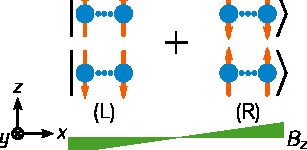
\includegraphics[scale=1.2]{img/GM_double_well.pdf}
    \caption[Best entangled state for the spatial two-ensembles]{(blue-circle) Atoms located at (L) or (R).
    (red-arrow) Spin state of each of the atoms.
    (green-area) Linear magnetic field $B_z$.
    Note that the $z$-axis is to represent the direction of the spins.
    On the other hand, the state is a linear superposition of the upper state and the lower state, represented by $\ket{\cdot}$ and $+$ sign.
    Note that all particles at (L) or (R) are assumed to be in the same spatial spot.}
    \label{fig:gm-double-well}
  \end{center}
\end{figure}

We compute first the $\qfif{\rho^{(\text{s})},j_z^{(n)},j_z^{(m)}}$ for $\ket{\Psi}$ as
\be
  \qfif{\ket{\Psi},j_z^{(n)},j_z^{(m)}}=\lcor
  \begin{aligned}
    & 4j^2  & &\quad \text{if} \quad (n,m)\in\text{(L,L) or (R,R)},\\
    & -4j^2 & &\quad \text{if} \quad (n,m)\in\text{(L,R) or (R,L)}.
  \end{aligned}
  \right.
\ee
Now, if we separate the terms of the sum in Eq.~\eqref{eq:gm-bound-for-insensitive-and-thermal-state} into two groups, such that one sum is for indexes $(n,m)\in\text{(L,L) or (R,R)}$, and the other is for indexes $(n,m)\in\text{(L,R) or (R,L)}$, we can compute the bound for the best state for the two ensemble case as
\be
\begin{split}
  \varian{b_1}_{\text{bs}}|_{\max} &=
  \sum_{\ver{(n,m)\in}{ \text{(L,L) or (R,R)}}} a^2 4j^2 + \sum_{\ver{(n,m)\in}{ \text{(L,R) or (R,L)}}} -a^2 (-4j^2)\\
  &= 4 a^2 N^2j^2.
\end{split}
\ee

On the other hand, if we compute now the standard deviation Eq.~\eqref{eq:gm-variance}, as we did before for the case of the chain Eq.~\eqref{eq:gm-variance-chain},
we have that for the two ensembles case $\mu=0$ and the standard deviation for the spatial state is
\be
  \sigma_{\text{te}}^2 = a^2,
  \label{eq:gm-variance-two-ensembles}
\ee
with which
\be
  \varian{b_1}_{\text{bs}}|_{\max} = 4 \sigma_{\text{te}}^2 N^2j^2.
\ee
Before concluding, we want to show another more usual approach to the same problem.

Knowing that the QFI is convex in the state and considering the spatial state to be Eq.~\eqref{eq:gm-double-well-spatial-pdf}, we reduce our problem to the internal subspace in which state that maximizes the QFI is the one that maximizes $(\Delta H_1)^2$.
In this case, taking into account the particle locations are given and that we have zero magnetic field at the origin, we obtain
\be
  H_{1,\text{eff}}^{(\text{s})} = a(\mtxid^{(\text{L})}\otimes J_{z}^{(\text{R})}-J_{z}^{(\text{L})}\otimes \mtxid^{(\text{R})}),
  \label{eq:gm-effective-hamiltonian-double-well}
\ee
where we write the effective Hamiltonian that the particles on the left and right feel.
This proves that we have used the right state, since it maximizes the variance $\varian{H_{1,\text{eff}}^{(\text{s})}}$ \cite{Landini2014}.

\subsubsubsection{States separable into $\ket{\psi}^{( \text{L})}\otimes\ket{\psi}^{(\text{R})}$}

Now that we have already introduced the reader to the case of the two ensembles, we take the opportunity to show some more important results for states of the form of $\ket{\psi}^{(\text{L})} \otimes \ket{\psi}^{(\text{R})}$.
These states can reach the Heisenberg limit, while they are easier to realize experimentally than states in which the particles on the left and particles on the right are entangled with each other.

First, we will compute the bound for states insensitive to the homogeneous field.
For such states we only have to compute the QFI for $H_{1,\text{eff}}$ Eq.~\eqref{eq:gm-effective-hamiltonian-double-well} such that
\be
  \varinv{b_1}|_{\max} = \qfif{\ket{\psi}^{(\text{L})}\otimes\ket{\psi}^{(\text{R})},a( \mtxid^{(\text{L})}\otimes J_{z}^{(\text{R})}-J_{z}^{(\text{R})}\otimes \mtxid^{(\text{L})})}= 2a^2\qfif{\ket{\Psi}^{(\text{L})},J_z^{(\text{L})}},
  \label{eq:gm-bound-insensitive-twoens-simplified}
\ee
where we used the general rule Eq.~\eqref{eq:bg-qfi-additive-for-tensor-product} and that any scalar multiplying the second argument of the QFI can be extracted outside the function squared.

Now, we analyze how the bound would look like for states sensitive to the homogeneous field.
Note that the single point correlation function for particles at "(L)" and "(R)" is $a$ and $-a$ respectively, and the two point correlation function is $a^2$ for both. Thus, in the case of computing the bound for the states sensitive to the homogeneous fields, we have that $F_{01}^{(\text{L})} = -F_{01}^{(\text{R})}$, which we used the superscript to indicate in this case over which subspace is computed the QFI matrix element, whereas the other two matrix elements we have to compute are equal for both subspaces "(L)" and "(R)".
The precision bound for states sensitive to the homogeneous fields is obtained as
\be
\begin{split}
\varinv{b_1} \leqslant &  F_{11}+\frac{(F_{01})^2}{F_{00}}\\
 =& F_{11}^{(\text{L})}+F_{11}^{(\text{R})} +\frac{(F_{01}^{(\text{L})}+F_{01}^{(\text{R})})^2} {F_{00}^{(\text{L})}+F_{00}^{(\text{R})}}\\
 =& 2F_{11}^{(\text{L})} +\frac{(F_{01}^{(\text{L})}-F_{01}^{(\text{L})})^2} {2F_{00}^{(\text{L})}}\\
 =& 2F_{11}^{(\text{L})}\\
 =& 2 a^2 \qfif{\rho^{(L)}, J_z^{(L)}},
\end{split}
\label{eq:gm-bound-sensitive-twoens-simplified}
\ee
where we use in the first line the identities for additions under tensor products Eqs.~\eqref{eq:bg-qfi-additive-for-tensor-product} and \eqref{eq:gm-FAB-additive-under-tensor}, and in the last line we extract the common factor $a^2$ and we use the linearity on the arguments the QFI.
Note that this is the same precision bound we will obtain for states insensitive to the homogeneous fields.
The reader may note that this bound relates how good the state on the "(L)" or "(R)" subsystem is in sensing the homogeneous field with the precision achievable for the gradient parameter.
This is reasonable because the state in "(L)" is not interacting neither correlated with "(R)".
Hence, after the homogeneous field is estimated for "(L)" and "(R)" independently,
the gradient can also be estimated as the difference between the two estimates divided by the square distance $a^2$.

In the literature one can find several states that can be used to measure homogeneous field, such as the GHZ states \cite{Greenberger1989}, unpolarized Dicke states, and spin-squeezed states.
Note that if $\ket{\Psi}$ is separable, then based in Eq.~\eqref{eq:bg-shot-noise-limit} and for any of the two bounds Eqs.~\eqref{eq:gm-bound-insensitive-twoens-simplified} and \eqref{eq:gm-bound-sensitive-twoens-simplified}, we have
\be
  \qfif{\ket{\Psi}_{\text{sep}}^{(\text{L})}\ket{\Psi}_{\text{sep}}^{(\text{R})},\,a(J_z^{(\text{L})} \mtxid^{(\text{R})}-\mtxid^{(\text{L})} J_z^{(\text{R})})}
  = 2a^2\qfif{\ket{\Psi}_{\text{sep}}^{(\text{L})}, J_z^{(\text{L})}}
  = 2a^24\frac{N}{2}j^2
  \leqslant 4a^2Nj^2.
  \label{eq:gm-snl-two-ensembles}
\ee
Note that each of the ensembles has half of the total particle number $N$.
Eq.~\eqref{eq:gm-snl-two-ensembles} can be seen as the SNL when two ensembles are used for gradient metrology.
In Table~\ref{tab:result-states-two-ensembles}, we summarized the precision bounds for states of type $\ket{\Psi}^{(\text{L})}\otimes \ket{\Psi}^{(\text{R})}$ for the two-ensemble case.
\begin{table}
  \begin{center}
    \begin{tabular}{|l|c|c|}
    \hline
    States in (L) and (R) & $\qfif{\rho,J_z}$ for $N/2$ & $(\Delta b_1)^{-2}\leqslant$ \\
    \hline
    $\ket{+j}_l^{\otimes N/2} \otimes \ket{+j}_l^{\otimes N/2} $ & $Nj$ & $ 2a^2Nj$ \\
    \hline
    %$ \ket{\text{SpSq}}\otimes\ket{\text{SpSq}}$ &  & \\
    %\hline
    $\ket{\ghz}\otimes\ket{\ghz}$ & $N^2/4$ & $ a^2N^2/2$\\
    \hline
    $\ket{\dicke{{N/2}}}_{x}\otimes \ket{\dicke{{N/2}}}_{x}$ & $N(N+4)/8$ & $ a^2N(N+4)/4$\\
      \hline
    $\ket{\Psi}_{\text{sep}}\otimes\ket{\Psi}_{\text{sep}}$ & $2Nj^2$  & $ 4a^2Nj^2$ \\
    \hline
    \end{tabular}
  \end{center}
\caption{(first column) The complete state as a tensor product of the state in (L) and the state in (R). Note that for the GHZ state and the unpolarized Dicke state, the spin is $j=\frac{1}{2}$.
The last state $\ket{\Psi}$ is the best separable state for the estimation of the homogeneous field.
Hence, the bound for $\ket{\Psi}$ coincides with the SNL for gradient metrology with two ensembles.
(second column) Precision of the estimation of the homogeneous magnetic field in one of the ensembles.
(third column) From the second column and based on Eqs.~\eqref{eq:gm-bound-insensitive-twoens-simplified} and \eqref{eq:gm-bound-sensitive-twoens-simplified}, we compute the precision for differential magnetometry for various product quantum states in two ensembles spatially separated from each other by a distance $a$.
Note that all states are sensitive to the homogeneous field so the saturability of of the bound is not ensured.
This is the reason we use "$\leqslant$" instead of "$|_{\max}$".
}
\label{tab:result-states-two-ensembles}
\end{table}

In this section we have shown to the reader how one should handle the spatial width of the system for classifying it for gradient metrology as well as a state-of-the-art system in which the Heisenberg limit is achieved. Moreover, we have sown how to use the tools developed on previous section to compute simple bounds. In the next section we will focus on single cold-atoms ensembles since the play an important role on todays quantum technology and experiments and many groups are trying to realize them whit great success but with few theoretical support from our point of view.

%%%%%%%%%%%%%%%%%%%%%%%%%%%%
\subsection{Magnetometry with an atomic ensemble}
\label{sec:gm-single-cloud}
%%%%%%%%%%%%%%%%%%%%%%%%%%%%

In this section, we discuss magnetometry with a single
atomic ensemble in more detail.
We consider a one-dimensional ensemble of spin-$j$ atoms
placed in a one dimensional trap, which is elongated
in the  $x$-direction.
The magnetic field points in the $z$-direction,
and has a constant gradient along the $x$-direction.
The setup is depicted
in Fig.~\ref{fig:gm-single-ensemble-in-gradient}.
In the last part of this section, we calculate precision bounds for the
gradient estimation for some important multi-particle quantum states,
for instance, Dicke states or GHZ states.
Note that all these states are PI, since we
assume that a PI procedure prepared the states.
\begin{figure}[htp]
  \begin{center}
  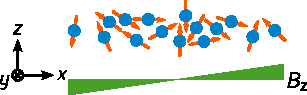
\includegraphics[scale=1.2]{img/GM_single_cloud.pdf}
  \caption[Single atomic ensemble for gradient magnetometry]{(blue-point) Atomic ensemble with their spins (red-arrow) pointing randomly in any direction coupled with a linear magnetic field $B_z$ (green).
  The spatial state $\rho^{(\text{x})}$ is assumed to be permutationally invariant.
  The ensemble is centered around the place at which the magnetic field is null due to the invariance of the precision bound under translations of the system.}
  \label{fig:gm-single-ensemble-in-gradient}
  \end{center}
\end{figure}

%%%%%%%%%%%%%%%%%%%%%%%%%%%
\subsubsection{Precision bound for an atomic ensemble}
%%%%%%%%%%%%%%%%%%%%%%%%%%%

In an atomic ensemble of very many atoms, typically
the atoms cannot be individually addressed.
This can be taken into account, if we consider
quantum states that are PI.
Hence, we will consider states for which both the internal state $\rho^{(\text{s})}$ and the probability distribution function
$\prob(\bs{x})$, appearing in Eq.~(\ref{eq:gm-thermal-state}),
are PI.
The permutational invariance of $\prob(\bs{x})$ implies that
\be
  \label{eq:pi-for-pdf}
  \prob(\bs{x})=\tfrac{1}{N!}\sum_{k}\mathcal{P}_k [\prob(\bs{x})],
\ee
where the summation is over all the possible permutations of the variables $x_n$ denoted by $\mathcal{P}_k$.

As we have shown in Section~\ref{sec:gm-cramer-rao-bounds}, the precision bound is invariant under spatial translations.
This allows us to place the "center of mass" of the system at the origin of the coordinate system.
With this simplifying assumption and based on Eqs.~\eqref{eq:gm-mean}, \eqref{eq:gm-variance} and \eqref{eq:gm-correlation}, the single-point average appearing in Eq.~\eqref{eq:gm-bound-for-sensitive-and-thermal-state} is
\be
  \int x_n \prob(\bs{x}) \, \text{d}^N\bs{x} = \int \frac{\sum_{n=1}^N x_n}{N} \prob(\bs{x}) \, \text{d}^N\bs{x} = \mu = 0,
  \label{eq:gm-single-point-average-sinens}
\ee
where we used the permutational invariance of $\prob(\bs{x})$ substitute $x_n$ by the sum appearing in Eq.~\eqref{eq:gm-mean}.
In a similar way we obtain
\be
  \int x_n x_m \prob(\bs{x}) \, \text{d}^N\bs{x} = \lcor
  \begin{aligned}
    &\sigma^2         &&\quad\text{for}\quad n=m,\\
    &\frac{\eta}{N-1} &&\quad\text{for}\quad n\neq m,
  \end{aligned}\right.
  \label{eq:gm-two-point-correlation-sinens}
\ee
where we used that the system is placed at the origin $\mu=0$.
An interesting property of the covariance of this type is that its a value is bounded from below and from above by the variance itself and the particle number $N$ in the following way,
\be
  \frac{-\sigma^2}{N-1}\leq \eta\leq \sigma^2.
\ee
Note that in the first sum in Eq.~\eqref{eq:gm-bound-for-sensitive-and-thermal-state} there are in total $N(N-1)$ terms proportional to $\eta/(N-1)$ and $N$ terms proportional to $\sigma^2$.

From the linearity in the second and third arguments of $\qfif{\rho, A, B}$ Eq.~\eqref{eq:gm-FAB} and for states insensitive to the homogeneous field, where $\qfif{\rho, J_z}=0$, we have that
\be
  \sum_{n=1}^N \qfif{\rho, j_z^{(n)}} = -\sum_{n\neq m}^N \qfif{\rho,j_z^{(n)},j_z^{(m)}}.
  \label{eq:gm-qfi-identity-insensitive}
\ee


From the definition of the QFI for states insensitive to the homogeneous field, Eq.~\eqref{eq:gm-bound-for-insensitive-and-thermal-state}, we compute the bound for single ensembles as
\be
\begin{split}
  (\Delta b_1)^{-2}|_{\max} &= \sum_{n,m}^N \int x_n x_m \prob(\bs{x}) \, \text{d}^N\bs{x} \qfif{\rho^{(\text{s})}, j_z^{(n)}, j_z^{(m)}}\\
  &=\sum_{n=1}^N \sigma^2 \qfif{\rho,j_z^{(n)}} + \sum_{n\neq m}^N \eta \qfif{\rho,j_z^{(n)},j_z^{(m)}}.
\end{split}
\ee
Together with Equation~\eqref{eq:gm-qfi-identity-insensitive} we write the precision bound for states insensitive to the homogeneous fields as
\be
(\Delta b_1)^{-2}|_{\max} = (\sigma^2-\eta) \sum_{n=1}^{N} \qfif{\rho^{(\text{s})},j_z^{(n)}}.
\label{eq:gm-bound-insensitive-sinens}
\ee
Note that the bound in Eq.~\eqref{eq:gm-bound-insensitive-sinens}
can be saturated by an optimal measurement.
Nevertheless, it cannot surpass the
shot-noise scaling, $\sim N$, because $\qfif{\rho^{(\text{s})},j_z^{(n)}}$, the QFI for the single-particle operator $j_z^{(n)}$, cannot be larger than $j^2$.

To compute the bound for states sensitive to the homogeneous field, note that in the second term appearing in Eq.~\eqref{eq:gm-bound-for-sensitive-and-thermal-state} is proportional to the single-point average Eq.~\eqref{eq:gm-single-point-average-sinens} which was chosen to be equal to zero.
Hence, we only have to compute the first term of the Eq.~\eqref{eq:gm-bound-for-sensitive-and-thermal-state} as
\be
\begin{split}
  \varinv{b_1}\leqslant& \sum_{n,m}^N \int x_n x_m \prob(\bs{x}) \, \text{d}^N\bs{x} \qfif{\rho^{(\text{s})}, j_z^{(n)}, j_z^{(m)}}\\
  =& \sum_{n=1}^N \sigma^2 \qfif{\rho,j_z^{(n)}} + \sum_{n\neq m}^N \eta \qfif{\rho,j_z^{(n)},j_z^{(m)}}\\
  =&(\sigma^2- \eta)\sum_{n=1}^N  \qfif{\rho,j_z^{(n)}} + \eta\sum_{n, m}^N  \qfif{\rho,j_z^{(n)},j_z^{(m)}},
\end{split}
\ee
where in the second line we compute the diagonal and the off-diagonal terms of the sum separately and in the last line we add $\eta\sum_{n=1}^N \qfif{\rho,j_z^{(n)}}$ to the last term and subtract it from the first term to make the expression more similar to Eq.~\eqref{eq:gm-bound-insensitive-sinens}.

Hence, for states sensitive to homogeneous fields,
the precision of estimating the gradient is bounded from above as
\be
\label{eq:gm-bound-sensitive-sinens}
\varinv{b_1} \leqslant (\sigma^2-\eta) \sum_{n=1}^N \qfif{\rho^{(\text{s})},j_z^{(n)}} + \eta \qfif{\rho^{(\text{s})},J_z}.
\ee
The second term on the right-hand side of Eq.~\eqref{eq:gm-bound-sensitive-sinens} is new in the sense that it did not appear in the bound for states insensitive to homogeneous fields.
Note that the bound in Eq.~(\ref{eq:gm-bound-sensitive-sinens}) is not necessarily saturable if the optimal measurements to estimate the gradient parameter and the homogeneous parameter do not commute with each other.
Note that even if the first term cannot overcome the SNS, in the second term the covariance is multiplied by QFI for estimating the homogeneous field and therefore this concrete term can make the bound, for extremely correlated particle positions, to scale as HS.

%%%%%%%%%%%%%%%%%%%%%%%
\subsubsection{Precision limit for various spin-states}
%%%%%%%%%%%%%%%%%%%%%%%

In this section, we present the precision limits for different classes of important quantum states such as the totally polarized state, the state having the largest precision among separable states, or the singlet state.
We will calculate the precision bounds presented before, Eqs.~\eqref{eq:gm-bound-insensitive-sinens} and \eqref{eq:gm-bound-sensitive-sinens}, for these systems.
We show first the results for singlets that are insensitive to homogeneous
fields.
In this case, the bounds can be achieved by choosing
the appropriate magnitude to measure.
The rest of the results are for states sensitive to homogeneous
fields which in general are not necessarily achievable bounds.

Before going into the details of our computations we present a summary of the results obtained in this section.
The summary for different states can be found in the Table~\ref{tab:compare all the states}.
\begin{table}
  \begin{center}
  \begin{tabular}{|l|c|}
    \hline
    States & $\varinv{b_1}$ \\
    \hline
    PI singlet states & $ |_{\max} = (\sigma^2-\eta) \frac{4Nj(j+1)}{3}$ \\
    \hline
    $\ket{+j}_{y}^{\otimes N}$ & $\leqslant \sigma^2 2Nj$ \\
    \hline
    Best separable state $\ket{\Psi}$ & $\leqslant \sigma^2 4N j^2$ \\
    \hline
    $\ket{\dicke{N}}_{z}$ & $ |_{\max}=(\sigma^2-\eta) N$\\
    \hline
    $\ket{\dicke{N}}_{x}$ & $ \leqslant (\sigma^2 -\eta) N + \eta \frac{N(N+2)}{2}$ \\
    \hline
    $\ket{\ghz}$ & $\leqslant (\sigma^2 - \eta) N  + \eta N^2$ \\
    \hline
  \end{tabular}
  \end{center}
\caption[Bounds on the precision for different internal states for gradient magnetometry.]{Precision bounds for  differential magnetometry for various quantum states.
For the definition of the states, see the text.
If the bound are proved to be saturable then
the \"max\" subscript is used instead of an inequality.}
\label{tab:compare all the states}
\end{table}

%%%%%%%%%%%%%%%%%%%%%%%
\subsubsubsection{Singlet states}
%%%%%%%%%%%%%%%%%%%%%%%

We consider now the singlet state, which is invariant under the influence
of a homogeneous field along any direction.
So, we have to compute the formula for the bound of the precision Eq.~(\ref{eq:gm-bound-insensitive-sinens}).
A pure singlet state is an eigenstate of the collective $J_z$ and $J^2$
operators, with an eigenvalue zero in both cases.
There are many different singlet states for an ensemble of $N$
spin-$j$ particles, which some of them are PI.
Surprisingly the precision bound we compute is the same
for any PI singlet.
Atomic ensembles in a singlet state have been experimentally
created with cold gases \cite{Toth2010, Behbood2014}.

In an $N$-particle system, there are several singlets pairwise orthogonal to each other.
The number of such singlets, $D_0$, depends on the particle spin $j$ and the number of particles $N$.

The most general singlet state can be written in the total angular momentum basis, using $D$ to label the degenerate states, see Appendix~\ref{app:angular-subspaces}.
In its eigenbasis the singlet is written as
\be
\rho^{(\text{s})}=\sum_{D=1}^{D_0}\lambda_D\ketbra{0,0,D}{0,0,D},
\label{eq:gm-general-singlet}
\ee
where $\sum_D \lambda_D=1$.
In its complete form the eigenvalues of the spin density matrix are $\lambda_{J,M_z,D}=\delta_{0,J}\lambda_D$.

Looking at Eq.~\eqref{eq:gm-bound-insensitive-sinens},
we must compute the QFI for the one-particle operator $j_z^{(n)}$ in order to compute the precision bound for PI singlet states.
For that purpose we use the fact that when $j_z^{(n)}$ acts on a singlet state, it produces a state outside of the singlet subspace.
This can be proved by noting that
\be
  e^{i \pi J_x} j_z^{(n)} e^{-i \pi J_x}=-j_z^{(n)}
\ee
and that $e^{-i\pi J_x} \ket{0,0,D} = \ket{0,0,D}$
holds for any pure singlet state.
Hence, we can arbitrarily flip the sign of $j_z^{(n)}$ so
\be
  \bra{0,0,D}{j_z^{(n)}}\ket{0,0,D'}
  =-\bra{0,0,D}{j_z^{(n)}}\ket{0,0,D'},
\ee
which implies
\be
  \bra{0,0,D}{j_z^{(n)}}\ket{0,0,D'}=0,
  \label{eq:gm-expectation-jzn-for-singlets}
\ee
for any pair of pure singlet singlet states.

In order to compute the QFI for the singlet state we use
Eq.~\eqref{eq:gm-FAB-rewrite-with-trace}.
Hence, we can write the following for the second term on Eq.~(\ref{eq:gm-FAB-rewrite-with-trace}),
\be
  8\sum_{D,D'}
  \tfrac{\lambda_D\lambda_{D'}}
  {\lambda_D+\lambda_{D'}}
  |\bra{0,0,D}{j_z^{(n)}}\ket{0,0,D'}|^2=0.
\ee
It follows that the QFI of $j_z^{(n)}$ for any singlet is indeed simply
\be
  \label{eq:gm-qfi-as-trace-singlet}
  \qfif{\rho^{(\text{s})}, j_z^{(n)}}
  =4\tr({\rho^{(\text{s})} (j_z^{(n)})^2}).
\ee

Finally, we must compute the expectation value of the operator $(j_z^{(n)})^2$.
For that we have that
\be
  \tr(\rho^{(\text{s})}(j_k^{(n)})^2)
  =\tr(\rho^{(\text{s})}(j_l^{(n)})^2),
\ee
for any pair $k,l\in x,y,z$ due to the rotational invariance of the singlet, i.e, all the singlets remain invariant under a $SU(2)$ transformation of the kind $U=e^{i\phi J_{\bs{n}}}$, where $\bs{n}$ is an unitary vector belonging to the positional space.
Then we can write that
\be
\expect{(j_x^{(n)})^2+(j_y^{(n)})^2+(j_z^{(n)})^2}=j(j+1),
\ee
for any state, since it represents the spin number of the particle, which is fixed.
Hence, the expectation value of $(j_z^{(n)})^2$ on the singlet is
\be
  \label{eq:gm-expectation-jzn2-for-singlets}
  \tr(\rho^{(\text{s})}(j_z^{(n)})^2)=\frac{j(j+1)}{3},
\ee
for all the singlets.
Inserting this into Eq.~\eqref{eq:gm-qfi-as-trace-singlet} and using Eq.~\eqref{eq:gm-bound-insensitive-sinens}, we
obtain
\be
  \label{eq:gm-precision-singlet}
  (\Delta b_1)^{-2}|_{\max} =\lpar\sigma^2-\eta\rpar \frac{4Nj(j+1)}{3}.
\ee

To conclude, singlet states are insensitive to homogeneous magnetic fields, hence determining the gradient leads to a single-parameter estimation problem.
This implies that there is an optimal operator that saturates the precision bound given by Eq.~\eqref{eq:gm-precision-singlet}.
However, it is usually very hard to find this optimal measurement,
although a formal procedure for this exists \cite{Paris2009, Ragy2016}.
In Ref. \cite{Urizar-Lanz2013}, a particular set-up for determining the magnetic gradient with PI singlet states was suggested by the measurement of the $J_x^2$ collective operator.
For this scenario the precision is given by the error propagation formula as
\be
\label{eq:gm- Jx2_acc}
(\Delta b_1)^{-2}
= \frac{|\partial_{b_1}\expect{J_x^2}|^2}{\expect{J_x^4}-\expect{J_x^2}^2}.
\ee

%%%%%%%%%%%%%%%%%%%%%%%
\subsubsubsection{Totally polarized state}
%%%%%%%%%%%%%%%%%%%%%%%

The totally polarized state can easily be prepared experimentally.
It has already been used for gradient magnetometry with a single atomic ensemble \cite{Koschorreck2011,Vengalattore2007}.
For the gradient measurement as for the measurement of the homogeneous field, the polarization must be perpendicular to the field we would like to measure in order to take advantage of the interaction between the particles and the field.
Here we chose as before the totally polarized state along the $y$-axis which is written as $\ket{j}_y^{\otimes N}$.
Note that this state is a state sensitive to the homogeneous field, hence, we must use the Eq.~(\ref{eq:gm-bound-sensitive-sinens}) to compute the bound.

For the pure states we have that $\qfif{\ket{\psi}, A} = 4(\Delta A)^2$.
Together with,
$(\Delta j_z^{(n)})^2=j/2$ and $(\Delta J_z)^2=Nj/2$, when the polarization is
perpendicular to the $z$-direction, the precision will be computed straightforward from Eq.~\eqref{eq:gm-bound-sensitive-sinens}.

Therefore, the Cram\'er-Rao bound fixes the highest value for the precision
of the totally polarized state as
\be
(\Delta b_1)^{-2}\leqslant \sigma^2 2Nj  .
\ee
Note that the precision bound for the totally polarized state
is smaller than that of the optimal separable state we present later on.
We can see clearly that the precision scales as $\mathcal{O}(N)$.

Let us now see, which quantities have to be measured to estimate the field gradient with a totally polarized state.
The homogeneous field rotates all spins by the same angle, while the gradient rotates the spin at different positions by a different angle.
Due to that, the homogeneous field rotates the collective spin, but does not change its absolute value.
On the other hand, the field gradient decreases the absolute value of the spin, since it has been prepared to be maximal, which has been used in Ref.~\cite{Behbood2013} for gradient magnetometry, see Figure~\ref{fig:ionchain-evolution}.

%%%%%%%%%%%%%%%%%%%%%%%
\subsubsubsection{The best separable state}
%%%%%%%%%%%%%%%%%%%%%%%

We will now turn our attention to the precision bound for all separable spin states.
It is useful to obtain this value so we have a direct comparison on what is the best classically achievable precision.
It will turn out that for $j>\frac{1}{2},$ it is possible
to achieve a precision higher than with the fully polarized state.
One has to take into account that if the state is insensitive to the homogeneous field the bound can be saturated for sure, and if the state is sensitive to homogeneous fields, it would depend on the measurements compatibility and on the system as we discussed before.
From another point of view and instead of using the Eqs.~\eqref{eq:gm-bound-insensitive-sinens} and \eqref{eq:gm-bound-sensitive-sinens}, what we have is that the bound is the same $\qfif{\rho, H_1}$ for both cases.
Note that we can place the system at the point in which the magnetic field is null without changing the result.
Thus, it is easy to argue that the precision bound itself is a convex function on the states.
Moreover, it is also a convex function of the states when the external state $\rho^{(\text{x})}$ is fixed and only the internal $\rho^{(\text{s})}$ is considered.

In the single ensemble configuration, Eq.~\eqref{eq:gm-f11-thermal} must be computed only, where the two point correlation function returns $\sigma^2$ or $\eta$ based on Eq.~\eqref{eq:gm-two-point-correlation-sinens}.
On the other hand, for pure states we have that $\qfif{\rho^{(\text{s})}, j_z^{(n)}, j_z^{(m)}}$ is four times the correlation $\expect{j_z^{(n)}j_z^{(m)}}-\expect{j_z^(n)}\expect{j_z^{(m)}}$.
If the state is a product state, then we have  $\expect{j_z^{(n)}j_z^{(m)}}-\expect{j_z^(n)}\expect{j_z^{(m)}}=0$ for all $n\neq m$.
Hence, $\eta$ does not play any role in the precision.
Finally, we have to maximize only the variance of each of the single particle operators $4(\Delta j_z^{(n)})^2$.
From the definition of the variance,
\be
  \varian{j_z^{(n)}} = \expect{(j_z^{(n)})^2}-\expect{j_z^{(n)}}^2.
\ee
Hence, We try a state that approaches to zero its polarization on the $z$-direction and maximizes \expect{(j_z^{(n)})^2}.

We have that  $\ket{\Psi}=(\ket{+j}+\ket{-j})/\sqrt{2}$ is ideal for this, for any $j$.
Hence, we write the entire internal state as $\rho^{(\text{s})} =(\ketbra{\Psi}{\Psi})^{\otimes N}$.
This state gives $(\Delta j_z^{(n)})^2=j^2$ which can be used in Eq.~\eqref{eq:gm-f11-thermal} after multiplying by four.
Note that this state is permutationally invariant, hence we have finished the search for the best separable PI state.
Moreover, the state is sensitive to the homogeneous field.

Finally, the best achievable precision for separable states is written as
\be
  \varinv{b_1} \leqslant  \sigma^2 4N j^2,
  \label{eq:gm-best_separable}
\ee
where the state itself is sensitive to homogeneous fields.
This bound coincides with the totally polarized state studied before when the spin number $j=\frac{1}{2}$.

In the following we try to find a better precision bound making use of presumably better entangled states.
Note that the bound for the singlet state, even if it is entangled, is above the bound for the totally polarized state but below of the bound defined for the best separable state.
Nevertheless, when the singlet state is used effect of the homogeneous magnetic field has not to be compensated since it is insensitive to it and thus the bound can be saturated with an optimal estimator for the gradient field.

%%%%%%%%%%%%%%%%%%%%%%%
\subsubsubsection{The unpolarized Dicke states $\ket{\dicke{N}}_z$ and $\ket{\dicke{N}}_x$}
%%%%%%%%%%%%%%%%%%%%%%%

Unpolarized Dicke states play an important role in quantum optics and quantum information science.
The unpolarized Dicke state $\ket{\dicke{N}}_l$ with a maximal $\expect{J_x^2+J_y^2+J_z^2}=\mathcal{J}_{N/2}$, defined in Eq.~\eqref{eq:app-maximum-total-angular-momentum}, and $\langle J_l\rangle=0$ for any $l\in x,y,z$ is particularly interesting due to its entanglement properties and its metrological usefulness.
This state has been created in photonic experiments \cite{Kiesel2007,Wieczorek2009,Chiuri2012} and in cold atoms \cite{Luecke2011,Hamley2012}, while a Dicke state with $\langle J_z\rangle>0$ has been created with cold trapped ions \cite{haeffner2005}.

The Dicke state $\ket{\dicke{N}}$, the subscript when omitted stands for $z$,  is an eigenstate of $J_z$ so insensitive to homogeneous magnetic field pointing into the $z$-direction, thus the precision can be saturated by some measurement.
Whereas, The Dicke state $\ket{\dicke{N}}_x$ is sensitive to the homogeneous field.
Moreover it is very useful for homogeneous magnetometry as it has been shown in Ref.~\cite{Holland1993}.
Here we consider large particle numbers, to make the results simpler.

Since both Dicke states are pure, and following the procedure we used in previous sections, we have that to compute all the $\qfif{\rho^{(s)},j_z^{(n)}}=4(\expect{j_z^{(n)}j_z^{(m)}}-\expect{j_z^{(n)}}\expect{j_z^{(m)}})$ and $\qfif{\rho^{(s)},J_z}$ appearing in Eqs.~\eqref{eq:gm-bound-insensitive-sinens} and \eqref{eq:gm-bound-sensitive-sinens}.
Since both states are unpolarized and PI, we have that $\expect{J_z}=0$ $\expect{j_z^{(n)}}=0$ for both cases
Therefore, we only need to compute the second moments to compute the needed variances.

To distinguish between the to cases, $\ket{\dicke{N}}$ and $\ket{\dicke{N}}_x$, we will denote their expectation values by $\expect{\cdot}_{\dicke{}}$ and $\expect{\cdot}_{\dicke{},x}$, respectively.

First of all, from the definition of the Dicke states we have that
\be
  \expect{J_x^2+J_y^2+J_z^2} = \mathcal{J}_{N/2} = \frac{N}{2}\lpar\frac{N}{2}+1\rpar,
  \label{eq:gm-square-total-angular-momentum-dicke}
\ee
for both cases.
We have that $\expect{J_l^2}=0$ for $\ket{\dicke{N}}_l$.
The remaining of the second moments of Eq.~\eqref{eq:gm-square-total-angular-momentum-dicke} are equal among each other due to the rotational invariance of the states in the $l$-axis.
Hence, we can write that
\begin{subequations}
  \begin{align}
    \expect{J_z^2}_{\dicke{}} &= 0,\\
    \expect{J_z^2}_{\dicke{},x} &= \frac{\mathcal{J}_{N/2}}{2}.
  \end{align}
  \label{eq:gm-expect-jz2-both-dicke}
\end{subequations}
Invoking the rotational symmetry again, note that the single particle total spin operator is
\be
  \expect{(j_x^{(n)})^2+(j_y^{(n)})^2+(j_z^{(n)})^2}=\mathcal{J}_{1/2}
\ee
and that $\expect{J_l^2}=\sum_{n,m}^N \expect{j_l^{(n)}j_l^{(m)}}$, we arrive at
\begin{subequations}
  \begin{align}
    \expect{(j_z^{(n)})^2}_{\dicke{}}   &= \frac{1}{4},\\
    \expect{(j_z^{(n)})^2}_{\dicke{},x} &= \frac{1}{4},
  \end{align}
  \label{eq:gm-expect-jzn2-both-dicke}
\end{subequations}
after solving a system of linear equations.

Substituting Eqs.~\eqref{eq:gm-expect-jz2-both-dicke} and \eqref{eq:gm-expect-jzn2-both-dicke} into Eqs.~\eqref{eq:gm-bound-insensitive-sinens} and \eqref{eq:gm-bound-sensitive-sinens}, the bounds for unpolarized Dicke states insensitive to the homogeneous field and sensitive to the homogeneous field are
\begin{subequations}
  \begin{align}
    \varinv{b_1}_{\dicke{}}|_{\max} &= (\sigma^2 -\eta)N,
    \label{eq:gm-bound-dicke-insensitive} \\
    \varinv{b_1}_{\dicke{},x} &\leqslant (\sigma^2 -\eta)N + \eta \frac{N(N+2)}{2},
    \label{eq:gm-bound-dicke-sensitive}
  \end{align}
\end{subequations}
where Eq.~\eqref{eq:gm-bound-dicke-sensitive} shows in principal a HS behavior in the second term, whenever the particles are very correlated among each other in the position subspace.
This is due to the metrological enhancement for the sensing of the homogeneous field.
In the next section, we will see another example of a state useful for homogeneous field estimation that is useful for gradient magnetometry.

%%%%%%%%%%%%%%%%%%%%%%%
\subsubsubsection{The GHZ state}
%%%%%%%%%%%%%%%%%%%%%%%

The Greenberger-Horne-Zeilinger (GHZ) state is also highly entangled and plays an important role in quantum information theory \cite{Greenberger1990}.
They have been created experimentally in photonic systems \cite{Pan2000,Yao2012,Lu2007} and trapped ions \cite{Sackett2000,Monz2011}.

We invoke the definition of the GHZ states Eq.~\eqref{eq:lt-ghz-state} as
\be
  \ket{\ghz} = \tfrac{1}{\sqrt{2}}(\ket{0\cdots0}+\ket{1\cdots1}).
\ee
where $\ket{0}$ and $\ket{1}$ stands for particles with eigenvalue $-1/2$ and $+1/2$ respectively for the one-particle $j_z^{(n)}$ operator.
This state is very sensitive to the homogeneous field.

In order to calculate this bound explicitly, let us recall that for pure states the QFI is simplified to $\qfif{\rho,A}=4\varian{A}$ Eq.~\eqref{eq:bg-qfi-for-pure-states}.
Following the Eq.~\eqref{eq:gm-bound-sensitive-sinens}, for the GHZ state the expectation value of $j_z^{(n)}$ and
$J_z$ is equal to zero, and $\expect{(j_z^{(n)})^2}=\frac{1}{4}$ and $\expect{J_z^2}
= \frac{N^2}{4}$, which give the variances of $j_z^{(n)}$ and $J_z$ respectively.
Finally, we obtain the precision bound for gradient magnetometry for the GHZ state as
\be
\label{eq:gm-precision bound for ghz}
\varinv{b_1} \leqslant (\sigma^2 - \eta) N  + \eta N^2.
\ee
This means that we can reach the Heisenberg-limit with such states, but only in
cases where $\eta$ is positive, i.e, that the particles stay spatially correlated.


%%%%%%%%%%%%%%%%%%%%%%%%
\section[Conclusions]
{Conclusions}
\thiswatermark{\put(1,-241){\color{l-grey}\rule{84pt}{48pt}}
\put(84,-241){\color{grey}\rule{410pt}{48pt}}}


\section{Conclusions}
\thiswatermark{\put(1,-241){\color{l-grey}\rule{84pt}{48pt}}
\put(84,-241){\color{grey}\rule{410pt}{48pt}}}


\lettrine[lines=2, findent=3pt, nindent=0pt]{I}{n} this thesis we have presented some aspects of quantum metrology from three different perspectives.
Besides the introductory part, Chapters~\ref{sec:in} and \ref{sec:bg}, in Chapters~\ref{sec:vd}, \ref{sec:lt} and \ref{sec:gm}, our main results can be found.
In Chapter~\ref{sec:vd}, we have developed the theory of quantum metrology for metrology with noisy Dicke states.
In Chapter~\ref{sec:lt}, we have presented a method for witnessing the QFI with expectation values of some general observables.
Finally in Chapter~\ref{sec:gm}, we have computed precision bounds for gradient magnetometry.

The reader may notice that we have stressed the importance of bounding the quantum Fisher information based on some expectation values of some observables of the initial state.
As one can find in Chapters~\ref{sec:vd} and \ref{sec:lt}, we have pursued this idea.
It turns out that to compute the quantum Fisher information is not a trivial task and there is not measurement scheme to obtain it from the initial state apart from a complete tomography, which is a very demanding task for large system sizes.
Hence, some shortcuts to compute the bound of the QFI are necessary.

In Chapter~\ref{sec:vd}, we computed the precision bound for noisy unpolarized Dicke states based on some initial expectation values.
Moreover, we first reduced the number of expectation values needed to four.
More explicitly, we have to measure only the second and the fourth moments of the $y$-component and the $x$-component of the collective angular momentum in order to estimate the metrological usefulness of the system.
In practice, the fourth-order moments can also be well approximated by the second-order moments.
We note that after completing our calculations, we have recently became aware of a related work by Haine {\it et al} \cite{Haine2015}, which is based on the preliminary work in Ref.~\cite{Szigeti2014}.

In Chapter~\ref{sec:lt}, we developed a method based on the Legendre transform.
Based on this method, we are able to obtain a tight lower bound on the quantum Fisher information as a function of a set of expectation values of the initial state.
Furthermore, We tested our approach on extensive experimental data on photonic and cold gas experiments, and demonstrated that it works even for the case of thousands particles.
In the future, it would be interesting to use our method to test the optimality of various recent formulas giving a lower bound on the quantum Fisher information \cite{Zhang2014, Oudot2015}, as well as to improve the lower bounds for spin-squeezed states and Dicke states allowing for the measurement of more observables than the ones used in this publication.

On the other hand, in Chapter~\ref{sec:gm}, we have investigated the precision limits for measuring the gradient of a magnetic field with atomic ensembles arranged in different geometries and initialized in different states.
In particular, we studied spin-chain configurations as well as the case of two atomic ensembles localized at two different positions, and also the experimentally relevant set-up of a single atomic ensemble with an arbitrary density profile of the atoms was considered.
We discussed the usefulness of various quantum states for measuring the field strength and the gradient.
Some quantum states, such as singlet states, are insensitive to the homogeneous field.
Using these states, it is possible to estimate the gradient and saturate be Cramér-Rao bound, while for states that are sensitive to the homogeneous magnetic field, compatible measurements are needed for this task.
For spin chains and the two-ensemble case, the precision of the estimation of the gradient can reach the Heisenberg limit.
For the single ensemble case, only if strong correlation between the particles is allowed can the shot-noise limit be surpassed and even the Heisenberg limit be achieved.
However, even if the Heisenberg limit is not reached, single-ensemble methods can have a huge practical advantage compared to methods based on two or more atomic ensembles, since using a single ensemble makes the experiment simpler and can also result in a better spatial resolution.


%%%%%%%%%%%%%%%%%%%%%%%%
% REDEFINE TITLE FORMAT
%%%%%%%%%%%%%%%%%%%%%%%%
\titleformat{\section}[display]
{\vspace*{150pt}
\bf\Huge}
{{\textcolor{black}{\thesection}}. #1}
{0pt}
{}
[]
\titlespacing*{\section}{40pt}{10pt}{0pt}[40pt]


\appendix

\section{Long calculus appearing through the sections}
In this appendix we will develop long calculations appeared throughout different chapters.

\subsection[Simplification of the Eq.~{(\ref{eq:vd-result-before-simp})}]
{Simplification of $\expect{\{J_x^2,J_y^2\}+\{J_x,J_y\}^2}$}
\label{ap:loca-simplification}

The expectation value appearing on Equation~{(\ref{eq:vd-result-before-simp})} which we want to simplify has 6 different terms, all with two $J_x$ and another two $J_y$,
\be
  \expect{J_x^2J_y^2} + \expect{J_xJ_yJ_xJ_y} + \expect{J_xJ_y^2J_x}
  + \expect{J_yJ_x^2J_y} + \expect{J_yJ_xJ_yJ_x} + \expect{J_y^2J_x^2}.
\ee
From all those terms the third is somehow referent, since the pure unpolarised Dicke state used as reference is align with the $Ox$-axis, so $J_x\ket{D_N^{N/2}}_x=0$.

We use the commutation relations of the angular momentum operators $[J_k,J_l]=\epsilon_{klm} iJ_m$ to rearrange all operators,
\begin{subequations}
\begin{align}
  \expect{J_x^2J_y^2} & = i\expect{J_xJ_zJ_y}+\expect{J_xJ_yJ_xJ_y},
  \label{eq:ap-simplification-1} \\
  \expect{J_xJ_yJ_xJ_y} & = i\expect{J_xJ_yJ_z}+\expect{J_xJ_y^2J_x},
  \label{eq:ap-simplification-2} \\
  \expect{J_xJ_y^2J_x} & = \expect{J_xJ_y^2J_x},
  \label{eq:ap-simplification-3} \\
  \expect{J_yJ_x^2J_y} & = i\expect{J_yJ_xJ_z} + \expect{J_yJ_xJ_yJ_x},
  \label{eq:ap-simplification-4} \\
  \expect{J_yJ_xJ_yJ_x} & = -i\expect{J_zJ_yJ_x} + \expect{J_xJ_y^2J_x},
  \label{eq:ap-simplification-5} \\
  \expect{J_y^2J_x^2} & = -i\expect{J_xJ_yJ_z} + \expect{J_yJ_xJ_yJ_x}.
  \label{eq:ap-simplification-6}
\end{align}
\end{subequations}
One may notice that with those relations is enough to see that we have six $\expect{J_xJ_y^2J_x}$, for instance, Equation~{(\ref{eq:ap-simplification-1})} is $i\expect{J_xJ_zJ_y}$ plus Equation~{(\ref{eq:ap-simplification-2})} which at the same time is $i\expect{J_xJ_yJ_z}$ plus Equation~{(\ref{eq:ap-simplification-3})}.
So each equation has at the end one $\expect{J_xJ_y^2J_x}$ plus or minus some expectation value of the product of three operators.

If we sum all again, and we subtract $6\expect{J_xJ_y^2J_x}$ we will end with those three operator expectation values. They look like follows,
\be
  i\expect{J_xJ_zJ_y}+2i\expect{J_xJ_yJ_z}+i\expect{J_yJ_xJ_z}-3i\expect{J_zJ_yJ_x}-i\expect{J_xJ_yJ_z}.
\ee
Again using the commutation relations we can further simplify this expression.


\section{Miscellaneous mathematical tools}
In this appendix we will illustrate basic mathematical tools used all through the thesis.
They are shown here because without been figures of merit of the conceptual parts involving this thesis, they are nowadays sufficiently important for any whose intention is t expertise on this field of Quantum Metrology and Quantum Information.

\subsection{Hirusimi distribution and the Bloch sphere}

The Hirusimi distribution is a quasi-probabilistic distribution defined as
\be
  Q(\alpha) = \braopket{\alpha}{\varrho}{\alpha}
\ee
where ...

It is very common to express the particle density.

\subsection{Angular momentum subspaces for different spins}
\label{app:angular-subspaces}

Here I want to show how the whole Hilbert space of the spin angular-momentum of a multi-particle system splits. There are severas constituents such as the symmetric subspace, the PI subspace, the anti-symmetric subspace, etc.


\titleformat{\section}[display]
{\vspace*{150pt}
\bf\Huge}
{{\textcolor{black}{\thesection}}. #1}
{0pt}
{#1}
[]
\titlespacing*{\section}{40pt}{10pt}{40pt}[40pt]

\bibliography{biblio.bib}{}
\bibliographystyle{plain}

\end{document}
